%\documentstyle[graphicx,12pt]{article}
\documentclass[12pt]{article}
%\documentstyle[graphicx,epsfig,subfigure,12pt]{article}
\pagestyle{myheadings} \markright{ } \oddsidemargin 0in
\evensidemargin 0in \marginparwidth 40pt \marginparsep 10pt
%\topmargin 12pt %change from 0pt, since page numbers have to be inside 1"
%\headsep 24.12pt % .5in - 12pt (\headheight is 12pt)
%\footheight 1.0in
%\usepackage{color}
\textheight 8.5in \textwidth 6.3in
\renewcommand{\baselinestretch}{1.6}
\usepackage{latexsym}
\usepackage{amsmath}
\usepackage{amsfonts}
\usepackage{color}
%\usepackage[perpage,symbol]{footmisc}
\usepackage{amssymb}
\usepackage{psfrag}
\usepackage{graphicx}
\usepackage{amssymb}
\usepackage{multirow}
\newtheorem{theorem}{Theorem}
\newtheorem{lemma}{Lemma}
\newtheorem{proof}{Proof}[section]
\usepackage{verbatim}
\renewcommand{\thefootnote}{}
\begin{document}
%\begin{center}
\noindent {\Large\bf  {\color{red}{Goodness-of-fit Test for Partial Functional Linear Model with Errors in Scalar Covariates}}}% covariates Additive Measurement Error}

\vspace{0.2in}
\noindent     Tong Zhang$^{1,2}$, Zhihua Sun$^{1\dag} \footnote{\dag \baselineskip=12pt
 {\em Corresponding author.} }$ \ and \ Liuquan Sun$^{1,2}$
\vspace*{0.1in}

\noindent{\sl
$^1$University of Chinese Academy of Sciences, Beijing, 100049, P.R.China, \ \   sunzh@amss.ac.cn\\
}
\noindent{\sl
$^2$Institute of Applied Mathematics, Academy of
 Mathematics and Systems Science, Chinese Academy of Sciences,
 Beijing, 100190, P.R.China, \\ zt001062@mail.ustc.edu.cn \ \ slq@amt.ac.cn \\
}




\vspace{0.2in}

\noindent


%%%%%%%%%%%%%%%%%%%%%%%%%%%%%%%%%%%%%%%%%%%%%%%%%%%%%%%%%%%%%%%%%%%%%%%%%
\noindent{\bf Abstract.}
In this article, we study the {\color{red}{adequacy test}} of the partial functional linear model when the scalar predictor is measured with additive errors. Based on a corrected profile least-squares estimation of the null model,  estimated residuals are first constructed, and a
U-statistic-based test is proposed.  The asymptotic properties of the test are investigated under the null and the alternative hypotheses. It is shown that the proposed test can control the type I error well, and its power performance is satisfactory.
  The finite sample performance of the proposed  test is demonstrated through simulation studies and a real data analysis.
\vspace*{0.2in}

\noindent {\bf Keywords:}   Additive measurement error; Functional covariate; {\color{red}{Goodness-of-fit test}}; Partial functional linear model; U-statistic-based test.


% Running Head�� Estimation in a General  Hazards Regression Model
%%%%%%%%%%%%%%%%%%%%%%%%%%%%%%%%%%%%%%%%%%%%%%%%%%%%%%%%%%%%%%%%%%%%%%%%%
\newpage
\noindent{\large\bf 1. Introduction}
\vspace{0.1in}

In many fields,  emerging data often has the characteristic of trajectory, and is called functional data.  Horv{\'a}th and Reeder (2013) presented several typical examples of functional data. There has been a vast literature in the field of functional data analysis (FDA). Most of  the articles focus on the estimation of the   functional regression models.
\textcolor[rgb]{1.00,0.00,0.00}{ Morris (2015) classified functional regression models into three
categories: scalar
responses and functional predictors; functional responses
and scalar predictors; and functional responses and
functional predictors. Reiss et al. (2017) presented a comprehensive overview
of the first type regression models.}
For more details, we refer readers to Ferraty and Vieu (2007b); Ramsay and Silverman (2007); Hsing and Eubank (2015), and the references
therein.

\textcolor[rgb]{1.00,0.00,0.00}{It is well known that statistical inferences often depend  severely on correctly-specified models.  If the candidate models are not adequate, the subsequent statistical analysis results tend to be misleading. Therefore,  it is generally well recognized that the test of the  candidate model's suitability is  a fundamental and important topic.} In recent years, the adequacy test of regression models with functional covariate has
attracted increasing attention.
The earliest literature that focused on adequacy test of regression models with  functional covariate can be traced back to Cardot et al. (2003, 2004). \textcolor[rgb]{1.00,0.00,0.00}{Subsequently, the classic local test methods in H{\"a}rdle et al. (1998) and  Dette (1999) are applied to test the suitability of the functional linear model; see Delsol et al. (2011) and B{\"u}cher et al. (2011).  The global projection-based empirical process test in Escanciano (2006) is also extended to test the adequacy of the functional linear models (Garc{\'\i}a-Portugu{\'e}s et al., 2014). Recently, Cuesta-Albertos et al. (2019) and Patilea and S{\'a}nchez-Sellero (2020)
extended the residual marked empirical process test in Stute (1997) and  the U-statistic type test in Zheng (1996) to the functional data context, respectively.
%When functional variables are not considered, the last five existing works presented  classical methods for regression model test.
Besides, %\cite{horvath2013} investigated  the adequacy test of the  functional linear model against quadratic alternatives.
Hilgert et al. (2013) developed a minimax adaptive test for
the functional linear model.
However, all the above-mentioned works are limited to regression models with data observed accurately.}

In many applications, variables often inevitably  suffer from measurement errors owing to some causes (e.g. instrument imprecision, laboratory
uncertainties, human inconsistencies).
It is noted that measurement errors always cause misleading results, such as biased estimators and loss of efficiency.
There is a large body of literature on how to eliminate the adverse effects of measurement errors.
{\color{blue}
Sepanski and Lee (1995) and Tekwe et al. (2019) employed  a validation data set and  an instrumental variable to deal with measurement errors, respectively;
Sun et al. (2006) and Wang et al. (2020) developed nonparametric-correction approaches to  remove the disruptive  influence originated from measurement errors  when repeated measurements
or observations exist.}
However, as far as we know, there are only sporadic  existing studies on the treatment of  functional regression models with  measurement errors.
Radchenko et al. (2015) and Ferraty et al. (2019) developed estimating procedures for a functional
single index model and a nonparametric regression model when functional
predictors  suffer from measurement errors.
Zhu et al. (2019b) studied the partial functional linear model with real-valued covariates  measured with additive errors.
Zhu et al. (2019a) addressed the estimation of the semi-functional linear regression models when both functional- and
real-valued random variables are measured with additive errors.


In this article, for the candidate partial functional linear  model with  covariates  measured with additive errors, the model suitability is investigated with the aid of a U-statistic-based test,
{\color{blue}a basic introduction about U-statistic theories and U-statistic-based test can be found in Zheng (1996) and reference therein.
%It's worth pointing out that U-statistic-based test and empirical-process-based test are representative methods of local smoothing tests and global smoothing tests, respectively, and they are the two main categories of methods for model testing.
However, the complexity of constructing an appropriate test is doubled for the considered functional setting
due to the existence of the functional predictor and the variable with measurement error.}
\textcolor[rgb]{1.00,0.00,0.00}{The test statistic is built by combining local kernel smoothing method for both the scalar and the functional  predictors.
%A combining local kernel smoothing method for both the scalar and the functional predictors is employed to build a test statistic.
To the best of our knowledge, the present study is the first to apply  this local kernel method related to both  scalar  and  functional  predictors to test the model adequacy.}

\textcolor[rgb]{1.00,0.00,0.00}{Model adequacy test with measurement error has been considered challenging because of the main difficulties in calculating
the likelihood or forming residuals. See Ma et al. (2011) and Wang et al. (2020). In this study, we employ corrected profile least-squares method  to yield asymptotic unbiased estimators of the regression parameters. To eliminate the adverse effects due to measurement error, a U-statistic-based test statistic is constructed through a kernel weighting technique only related to the exactly-observed scalar predictor  and the functional variable. The developed test is free from  complex
 deconvolution operations or minimum  distance procedure, and therefore  possesses the advantage of  computational expedience.   }


The asymptotic properties of the  test statistic  under the null and the alternative hypothetical models are rigorously investigated.
We validate  that the proposed test can control the type I error well, along with  satisfactory power performance.
Numerical simulation and case analysis results show that the proposed method can effectively eliminate the adverse effects of measurement errors.

The remainder of this article is organized as follows. In Section 2, the model and test problem is introduced. In  Section 3,
{\color{blue} an estimation procedure of the null hypothetical model is presented,  and  an intuitive explanation why  the naive method fails is also listed.}
A corrected test procedure is proposed  in Section 4.  The asymptotic properties of the test and the determination of the critical value  are presented in Sections 5  and 6, respectively. Some simulation studies and a real data analysis are conducted in Sections 7 and 8. Some assumptions and technical proofs of the main results are collected in the Appendixes.

%%%%%%%%%%%%%%%%%%%%%%%%%%%%%%%%%%%%%%%%%%%%%%%%%%%%%%%%%%%%%%%%%%%%%%%%%
\vspace{0.3in}
\noindent{\large\bf 2.  Model and hypotheses}

\vspace{0.3in}
\noindent{\bf 2.1. Model introduction}
\vspace{0.1in}

Consider the partial functional linear model of the  following form:
$$
 Y=\mathbf{Z}^\top\beta+\int_{\mathfrak{T}}\alpha(t) X(t)dt+\varepsilon, \eqno{(1)}
$$
where $Y$ is a scalar response, $\mathbf{Z}$ is a $p$-dimensional  variable, and $\beta$ is  an unknown parameter vector. Both the {\color{blue}functional covariate} $X(\cdot)$ and the unknown slope function $\alpha(\cdot) $ are  smooth and square integrable functions defined on a bounded closed interval $\mathfrak{T}\subset \mathbb{R}.$  Without loss of generality, the interval $\mathfrak{T}$ is  assumed to be $[0,1].$ The variable $\varepsilon$ is the random model error with zero mean and finite variance $\sigma^{2}$.


Due to the existence of the measurement errors, the  covariate $\mathbf{Z}$ is unavailable.  Instead, a surrogate variable  $\mathbf{W}$ is observed. An  additive measurement error structure $\mathbf{W}=\mathbf{Z}+\mathbf{U}$ is assumed with a measurement error variable $\mathbf{U}$ of  zero mean  and   covariance matrix $\Sigma_{u}.$ Temporarily, $\Sigma_{u}$ is assumed to be  known, and the case of unknown $\Sigma_{u}$ will be discussed later. Furthermore, suppose that the measurement errors are caused by random rather than systematic factors,  and  the measurement error variable  $\mathbf{U}$ is independent of the variables $Y,$ $\mathbf{Z}$, and $X$.


\vspace{0.3in}
\noindent{\bf 2.2. The hypotheses}
\vspace{0.1in}

Estimation of model (1) has been addressed in Zhu et al. (2019b) via employing a  corrected profile least-squares estimating procedure. When the method in Zhu et al. (2019b) {\color{blue}is used for data analysis}, a fundamental and important question is to make sure that the model is appropriate. However, there is no existing  method to test the suitability of the candidate model in (1). This study aims for filling this gap by developing a U-statistic-based test procedure.

 To be specific, the test problem is stated as
$$
\mathcal{H}_{0}: \Pr\Big\{{\color{blue}{{\mathbb E}(Y|\mathbf{Z},X)}}=\mathbf{Z}^\top\beta+\int_{0}^{1}\alpha(t)X(t)dt\Big\}=1, \eqno{(2)}
$$
for some $ \beta \in  \mathbb{R}^{p} $ and some  slope function $\alpha \in \mathbf{L}^{2}[0,1].$ Here,  $\mathbf{L}^{2}[0,1]$ is a functional space composed  of all functions $f:[0,1]\rightarrow \mathbb{R}$ satisfying $\int_0^1 f^2(t)dt<\infty,$ with the norm {\color{red}{$\| f \|=\langle f,f\rangle^{1/2}$}} and the inner product $\langle f,g\rangle=\int_0^1 f(t)g(t)dt.$
Instead of  directional alternative hypotheses,
an omnibus alternative hypothesis is considered:
$$
\mathcal{H}_{1}:\Pr\Big\{{\color{blue}{{\mathbb E}(Y|\mathbf{Z},X)}}=\mathbf{Z}^\top\beta+\int_{0}^{1}\alpha(t)X(t)dt\Big\}<1, \eqno{(3)}
$$
for all  $\beta \in \mathbb{R}^{p}$ and  $ \alpha \in \mathbf{L}^{2}[0,1]$.


%%%%%%%%%%%%%%%%%%%%%%%%%%%%%%%%%%%%%%%%%%%%%%%%%%%%%%%%%%%%%%%%%%%%%%%%%

\vspace{0.3in}
\noindent{\large\bf 3.  Two related preliminaries}

\vspace{0.3in}
\noindent{\bf 3.1. Estimation of the null hypothetical model}
\vspace{0.1in}

Suppose that there is  a random sample  $\{(Y_{i}, \mathbf{W}_{i}, X_{i}),i=1,\ldots,n\}$ from $(Y,\mathbf{W}, X).$  Since  estimated model errors are often indispensable for a model diagnostic procedure, we first present an estimating method of the null hypothetical model.

\textcolor[rgb]{1.00,0.00,0.00}{Let $\gamma(s,t)= \texttt{cov}(X(s), X(t))$ be the covariance operator of the stochastic process $X.$ By Mercer's theorem,  the spectral decomposition of $\gamma(s,t)$ yields $\gamma(s,t)= \sum_{j=1}^\infty \lambda_j  \psi_j(s) \psi_j(t)$, where $\lambda_{1}\geq\lambda_{2}\geq\cdots\geq0$  are eigenvalues of $\gamma(s,t)$,  and  $\psi_{1}, \psi_{2}, \ldots  , $ are  eigenfunctions, which constitute an orthogonal basis  of the function space $\mathbf{L}^{2}[0,1].$ } Denote the empirical counterparts of  $\gamma(s,t),$ $\lambda_{j}$ and $\psi_{j}$  by $\hat{\gamma},$ $\hat{\lambda}_{j}$ and $\hat{\psi}_{j},$ for $j=1,2, \ldots .$

%Let $\gamma(s,t)= \text{cov}(X(s), X(t))$ be the covariance function of the stochastic process $X.$ By Mercer's theorem,  the spectral decomposition of $\gamma(s,t)$ yields $\gamma(s,t)= \sum_{j=1}^\infty \lambda_j  \psi_j(s) \psi_j(t)$, where $\lambda_{1}>\lambda_{2}>\cdots>0$  are eigenvalues of $\gamma(s,t)$,  and  $\psi_{1}, \psi_{2}, \ldots  , $ are  eigenfunctions, which constitute an orthogonal basis  of the function space $\mathbf{L}^{2}[0,1].$ Denote the empirical counterparts of  $\gamma(s,t),$ $\lambda_{j}$ and $\psi_{j}$  by $\hat{\gamma},$ $\hat{\lambda}_{j}$ and $\hat{\psi}_{j},$ for $j=1,2, \ldots .$

Let $Y=(Y_{1},\ldots,Y_ {n})^\top$ and $\mathbf{W}=(\mathbf{W}_{1},\ldots,\mathbf{W}_{n})^\top.$  Denote the identity matrix by $\textbf{I}.$   From Zhu et al. (2019b), the estimators of the regression parameter $\beta$ and the slope function $\alpha(t)$ are given by
$$
\hat{\beta}_n=\{\mathbf{W}^\top(\mathbf{I}-\mathbf{S})\mathbf{W}-n\Sigma_{u}\} ^{-1}\mathbf{W}^\top(\mathbf{I}-\mathbf{S})Y, \eqno{(4)}
$$
and
$$
\hat{\alpha}_n(t)=\displaystyle\sum_{i=1}^{m}\tilde{\alpha}_{i}\hat{\psi_{i}}(t),
$$
where  $\textbf{S}=\textbf{H}(\textbf{H}^\top \textbf{H})^{-1}\textbf{H}^\top,$ $\tilde{\alpha}=(\textbf{H}^\top \textbf{H})^{-1}\textbf{H}^\top(Y-\textbf{W}\hat{\beta}_n)=(\tilde{\alpha}_{1},\ldots,\tilde{\alpha}_{m})^\top,$ $\textbf{H}=(\hat{s}_{i,j})_{1\leq i \leq n, 1\leq j\leq m},$ and  $\hat{s}_{i,j}=\langle X_{i},\hat{\psi}_{j}\rangle$ for $1\leq i \leq n,$ $1\leq j\leq m.$ Herein, the cutoff parameter $m$ {\color{blue} is  the number of the highest eigenvalues/eigenfunctions selected, } and controls  the smoothness  degree  of the estimator $\hat{\alpha}_n(t)$.


The above estimating procedure offers an advantage that
 the estimators have closed forms. Thus, even if the data come from the alternative model, the estimated procedure and the follow-up test procedure can be carried out.

\vspace{0.3in}
\noindent{\bf 3.2. {\color{blue}{Intuitive explanation of the failure of the naive method}}}
\vspace{0.1in}

The method taking errors-in-variables  as  true variables is called a naive method.
Unfortunately, for the considered test problem in (2), the naive method  fails.

Denote the estimated naive model error  by $\hat{\varepsilon}_{ni}^{NA}=Y_i-\textbf{W}_{i}^\top\hat{\beta}_n^{NA}-\int_{0}^{1}\hat{\alpha}_n^{NA}(t)X_i(t)dt$ for $i=1, \ldots ,n,$ where $\hat{\beta}_n^{NA}$ and $\hat{\alpha}_n^{NA}(t)$ are the naive estimators of $\beta$ and $\alpha(t),$ respectively. {\color{blue} Similarly to the  proofs of Theorems 1 and 2 of  Zhu et al. (2019b), by some lengthy derivation,  it can be deduced that $\hat{\beta}_n^{NA}-\beta$ and $\hat{\alpha}_n^{NA}(t)-\alpha(t)$ have nonzero asymptotic means.  }
The estimated naive error can be decomposed into four parts:
\begin{eqnarray*}
&&\hat{\varepsilon}_{ni}^{NA}=
\left\{Y_{i}-\textbf{Z}_{i}^\top \beta-\int_{0}^{1}\alpha(t)X_i(t)dt\right\}-\mathbf{U}_{i}^\top\hat{\beta}_n^{NA}\cr&&  \hspace{1.2cm} +\int_{0}^{1}\{\alpha(t)-\hat{\alpha}_n^{NA}(t)\}X_i(t)dt+\textbf{Z}_{i}^\top(\beta-\hat{\beta}_n^{NA}),\ \ i=1, \ldots  ,n.
\end{eqnarray*}
Under the null hypothesis, {\color{blue} the expectations of the first two terms converge to zero. But the last two terms
 and therefore the naive error $\hat{\varepsilon}_{ni}^{NA}$
have nonzero asymptotic means because the naive estimators $\hat{\beta}_n^{NA}$ and  $\hat{\alpha}_n^{NA}(t)$ are asymptotically biased.}

The estimated naive  errors tend to  keep away from zero  under both the null and the alternative hypotheses. Therefore, the naive test cannot distinguish the null hypothetical model from the alternative ones. For the considered test problem, it is imperative to develop a corrected test procedure.

%%%%%%%%%%%%%%%%%%%%%%%%%%%%%%%%%%%%%%%%%%%%%%%%%%%%%%%%%%%%%%%%%%%%%%%%%
\vspace{0.3in}
\noindent{\large\bf 4. A corrected test procedure}
\vspace{0.1in}

Let  $\varepsilon=Y-\mathbf{Z}^\top\beta-\int_{0}^{1}\alpha(t)X(t)dt,$ and  $\mathbf{V}=(\mathbf{Z}^\top,X)^\top.$
The corrected model error is defined as  $\hat{\varepsilon}_{ni}=Y_i-\textbf{W}_{i}^\top\hat{\beta}_n-\int_{0}^{1}\hat{\alpha}_n(t)X_i(t)dt, \ i=1, \ldots  ,n,$ with $\hat{\beta}_n$ and $\hat{\alpha}_n(t)$ given in  Section 3. Further, denote $\check{K}_{h}(\mathbf{V}_{i},\mathbf{V}_{j})=k_{h_{0}}(d(X_{i},X_{j})){\color{red}{\displaystyle\prod_{l=1}^{p}k_{h_{l}}(\mathbf{Z}_{il}-\mathbf{Z}_{jl})}}$ for $i,j=1,\ldots,n.$ Herein,  $k_{h_l}(\cdot)$ is defined as $k(\cdot/h_l)$  with a univariate kernel function $k$ and  bandwidths $h_{l}, l=0, 1,\ldots, p.$ The metric {\color{red}{$d(X_1, X_2)=\Vert X_1-X_2 \Vert$}} is  defined on $\mathbf{L}^{2}[0,1]$.

The test methods arising from the estimated model errors are broadly categorized into two groups: local  tests  requiring  nonparametric local smoothing techniques  and global tests based on the weighted averages of residuals.
The U-statistic type test and the empirical process test are representative methods of the  local and the global methods, respectively.
It is generally agreed that  the U-statistic type test and the empirical process test {\color{blue} complement each other (Ma et al., 2014).
A comparison of the advantages and the disadvantages of these two methods can be found in Guo and Zhu (2017). Sun et al. (2021) pointed that the U-statistic type test and the empirical process test  are special cases of the ICM test with different weighting functions.}

{\color{blue}Following the line of Li and Wang (1998), we aim for developing a U-statistic type test for the considered hypothetical problem in (2). In general cases where $\varepsilon$ is a model error and $\mathbf{V}$ is a predictor, the U-statistic type test   originates from the equivalence of ${\mathbb E}[\varepsilon|\mathbf{V}]=0$ and ${\mathbb E}[\varepsilon{\mathbb E}(\varepsilon|\mathbf{V})\omega(\mathbf{V})]=0$
for some positive measurable weight function $w(v)$.}
Motivated by an estimator of {\color{blue}{${\mathbb E}[\varepsilon{\mathbb E}(\varepsilon|\mathbf{V})\omega(\mathbf{V})]$}},
define $\mathcal{T}^v_n$ as follows:
$$
\mathcal{T}^v_n=\displaystyle\frac{1}{n(n-1)}\frac{1}{\tilde{\varphi}(h)}\sum_{i=1}^{n}\sum_{j=1, j \neq i}^{n}\check{K}_{h}(\mathbf{V}_{i},\mathbf{V}_{j})\hat{\varepsilon}_{ni}\hat{\varepsilon}_{nj}, \eqno{(5)}
$$
where $\hat{\varepsilon}_{ni}$ is defined above.
The function $\tilde{\varphi}(h)$ is equal to $\psi(h_0)\displaystyle\prod_{l=1}^{p}h_{l},$ where  the  positive function $\psi(\cdot)$  is given in Assumptions (C3) in Appendix A.
However, $\mathcal{T}^v_n$ is  not calculable, because the variable $\mathbf{V}$ is unavailable.

A natural idea is replacing  the true variable $\mathbf{V}=(\mathbf{Z}^\top,X)^\top$ in (5) with the surrogate variable {\color{red}{$\mathbf{V}^{w}=(\mathbf{W}^{\top},X)^{\top}$.}}
Hence, we obtain a calculable statistic:
 \begin{eqnarray*}
\mathcal{T}^w_n=\displaystyle\frac{1}{n(n-1)}\frac{1}{\tilde{\varphi}(h)}\sum_{i=1}^{n}\sum_{j=1, j \neq i}^{n}{\color{red}{\check{K}_{h}(\mathbf{V}^{w}_{i},\mathbf{V}^{w}_{j})}}\hat{\varepsilon}_{ni}\hat{\varepsilon}_{nj}.
\end{eqnarray*}
 The statistic $\mathcal{T}^w_n$ is a consistent estimator of {\color{blue}{ ${\mathbb E}[\varepsilon{\mathbb E}(\varepsilon|\mathbf{V}^w)\omega(\mathbf{V}^w)]$ with some appropriate weight function. Observe that ${\mathbb E}[\varepsilon{\mathbb E}(\varepsilon|\mathbf{V}^w)\omega(\mathbf{V}^w)]$ $={\mathbb E}[{\mathbb E}^2(\varepsilon|\mathbf{V}^w)\omega(\mathbf{V}^w)].$
Under the null hypothesis,  we cannot judge  whether ${\mathbb E}[\varepsilon|\mathbf{V}^w],$ along with ${\mathbb E}[\varepsilon{\mathbb E}(\varepsilon|\mathbf{V}^w)\omega(\mathbf{V}^w)]$, is zero or not. Thus, the test $\mathcal{T}^w_n$ cannot control the type I error.}}

In practice,  measurement errors are commonly  known to occur in only one or several variables. Suppose that the first $q$ {\color{red}{$(0 \leq q \leq p)$}} components in  $\mathbf{Z}$ are observed accurately. Denote $\mathbf{\tilde{V}}=(\mathbf{\tilde{Z}}^\top, X)^\top$  with $\mathbf{\tilde{Z}}=(Z_1, \ldots  , Z_q)^\top.$ Under the null hypothesis, it is true that
{\color{blue}{${\mathbb E}[\varepsilon|\mathbf{\tilde{V}}]=0$}}, which yields {\color{blue}{${\mathbb E}[\varepsilon{\mathbb E}(\varepsilon|\mathbf{\tilde{V}})\omega(\mathbf{\tilde{V}})]=0.$}} Intuitively, the test  arising  from {\color{blue}{${\mathbb E}[\varepsilon|\mathbf{\tilde{V}}]$}}  should be able to control the type I error.

Based on the above considerations,
defined  $\mathcal{T}_n$ as follows:
$$
\mathcal{T}_n=\displaystyle\frac{1}{n(n-1)}\frac{1}{\varphi(h)}\sum_{i=1}^{n}\sum_{j=1,j \neq i }^{n}K_{h}(\mathbf{\tilde{V}}_{i},\mathbf{\tilde{V}}_{j})\hat{\varepsilon}_{ni}\hat{\varepsilon}_{nj},
$$
where $\varphi(h)=\psi(h_0)\displaystyle\prod_{l=1}^{q}h_{l},$ $K_{h}(\mathbf{\tilde{V}}_{i},\mathbf{\tilde{V}}_{j})=k_{h_{0}}(d(X_{i},X_{j})){\color{red}{\displaystyle\prod_{l=1}^{q}k_{h_{l}}(\mathbf{Z}_{il}-\mathbf{Z}_{jl})}}$ for $i,j=1,\ldots,n.$
The final test statistic is defined as
{\color{blue}
$$n\varphi(h)^{1/2}\mathcal{T}_n=\displaystyle\frac{1}{n-1}\frac{1}{\varphi(h)^{1/2}}\sum_{i=1}^{n}\sum_{j=1,j \neq i }^{n}K_{h}(\mathbf{\tilde{V}}_{i},\mathbf{\tilde{V}}_{j})\hat{\varepsilon}_{ni}\hat{\varepsilon}_{nj}.$$
}
The null hypothesis should be rejected when   $n\varphi(h)^{1/2}\mathcal{T}_n$ is large enough.

If the weight function {\color{blue}$\omega(\tilde{\mathbf{V}}_{i})$} is taken as
$\displaystyle\frac{1}{n-1}\sum_{j=1,j\neq i}^{n}$ $K_{h}(\mathbf{\tilde{V}}_{i},\mathbf{\tilde{V}}_{j}),$  $i=1, \ldots  ,n,$
then the test statistic  is actually the empirical estimator  of {\color{blue}{${\mathbb E}[\varepsilon{\mathbb E}(\varepsilon|\mathbf{\tilde{V}})\omega(\mathbf{\tilde{V}})]$}}  multiplied by a regularization factor $n\varphi(h)^{-1/2}.$
{\color{blue} Denote $$\hat{{\mathbb E}}(\varepsilon_{ni}|\mathbf{\tilde{V}}_i)=\dfrac{\sum_{j=1,j \neq i}^n\hat{\varepsilon}_{nj}K_{h}(\mathbf{\tilde{V}}_{i},\mathbf{\tilde{V}}_{j})}{\sum_{j=1,j \neq i}^n K_{h}(\mathbf{\tilde{V}}_{i},\mathbf{\tilde{V}}_{j})}.$$
To be specific, we can validate that
\begin{equation*}
\begin{aligned}
\hat{{\mathbb E}}[\varepsilon{\mathbb E}(\varepsilon|\mathbf{\tilde{V}})\omega(\mathbf{\tilde{V}})]&=: \dfrac 1 n \sum_{i=1}^n\hat{\varepsilon}_{ni} \hat{{\mathbb E}}(\varepsilon_{ni}|\mathbf{\tilde{V}}_i)\omega(\tilde{\mathbf{V}}_{i})\\
&= \dfrac 1 n \sum_{i=1}^n \hat{\varepsilon}_{ni} \dfrac{\sum_{j=1,j \neq i}^n\hat{\varepsilon}_{nj}K_{h}(\mathbf{\tilde{V}}_{i},\mathbf{\tilde{V}}_{j})}{\sum_{j=1,j \neq i}^n K_{h}(\mathbf{\tilde{V}}_{i},\mathbf{\tilde{V}}_{j})} \dfrac{1}{n-1}\displaystyle\sum_{j=1,j\neq i}^{n} K_{h}(\mathbf{\tilde{V}}_{i},\mathbf{\tilde{V}}_{j})\\
&=\dfrac {1} {n(n-1)}\sum_{i=1}^n\sum_{j=1,j \neq i}^n\hat{\varepsilon}_{ni}\hat{\varepsilon}_{nj}K_{h}(\mathbf{\tilde{V}}_{i},\mathbf{\tilde{V}}_{j}),\\
\end{aligned}
\end{equation*}
and thus,
$$n\varphi(h)^{-1/2} \hat{{\mathbb E}}[\varepsilon{\mathbb E}(\varepsilon|\mathbf{\tilde{V}})\omega(\mathbf{\tilde{V}})]=\displaystyle\frac{1}{n-1}\frac{1}{\varphi(h)^{1/2}}\sum_{i=1}^{n}\sum_{j=1,j \neq i }^{n}K_{h}(\mathbf{\tilde{V}}_{i},\mathbf{\tilde{V}}_{j})\hat{\varepsilon}_{ni}\hat{\varepsilon}_{nj}=n\varphi(h)^{1/2}\mathcal{T}_n.$$}This test statistic is of a relatively simple form, and the case of zero-denominator is effectively avoided. This technique is commonly used  in the local test methods (Li and Wang, 1998).

%%%%%%%%%%%%%%%%%%%%%%%%%%%%%%%%%%%%%%%%%%%%%%%%%%%%%%%%%%%%%%%%%%%%%%%%%
\vspace{0.3in}
\noindent{\large\bf 5. Asymptotic properties}
\vspace{0.1in}

For $\ t\in \mathbb{R}^+,$ denote the small ball centered at $X$ with radius $t$ by $\mathcal{B}(X,t)=\{X' \in \mathbf{L}^{2}[0,1]: d(X, X') \leq t\}.$ The small ball probability is defined as $p(t)=\Pr\{X' \in \mathcal{B}(X,t)\}$.

\vspace{0.1in}

\noindent{\bf Theorem 1.}  {\it
Under Assumptions  (C1)--(C6) in  Appendix A,  when the null hypothesis (2) holds, we have
$$
n\varphi(h)^{1/2}\mathcal{T}_n \xrightarrow{d}
\mathcal{N}(0, \sigma^2_{0}),
$$
with $\sigma^2_{0}$ presented in Appendix B.
}
\vspace{0.1in}

In the following, consider  the  local alternative hypotheses:
$$
\mathcal{H}_{1n}:Y=\mathbf{Z}^\top\beta+\int_{0}^{1}\alpha(t)X(t)dt+ \delta_n \mathcal{D}(\mathbf{Z},X)+\varepsilon, \eqno{(6)}
$$
where the deviation function $\mathcal{D}(\cdot,\cdot)$ satisfies
$${\color{blue}\displaystyle\inf_{\beta \in \mathbb{R}^p, \alpha(t)\in \mathbf{L}^{2}[0,1]}
{\mathbb E}\left\{ \mathcal{D}(\mathbf{Z},X)-\mathbf{Z}^\top \beta-\int_0^1\alpha(t)X(t)dt\right\}^2>0},$$
and $\delta_n$ is a constant.

\vspace{0.1in}

\noindent{\bf Theorem 2.}  {\it
Under the assumptions of Theorem 1, when the local alternative hypothesis (6) with $\delta_n=n^{-1/2}\varphi(h)^{-1/4}$ holds,  we have
$$
n \varphi(h)^{1/2}\mathcal{T}_{n} \xrightarrow{d} \mathcal{N}(\Lambda, \sigma^2_{0}),
$$
with $\Lambda$  and  $\sigma^2_{0}$ presented in Appendix B.
}
\vspace{0.1in}

Theorem 2 shows that the proposed test has nonignorable power for the alternative hypothesis (6). Even if the predictors suffer from  measurement errors, the proposed test has the same sensitivity as the method for accurately observed data.
In the following,  we investigate the convergence property of the  test under the fixed alternative hypothesis in (3).

\vspace{0.1in}

\noindent{\bf Corollary 1.}  {\it
Under Assumptions  (C1)--(C6) in  Appendix A, if the alternative hypothesis (3) holds, then $n\varphi^{1/2}(h)\mathcal{T}_n \rightarrow \infty,$ as $n\rightarrow\infty.$
}
\vspace{0.1in}

The existing {\color{red}{model testing}} methods for measurement error data often suffer from inconsistency (Wang et al., 2020). Theorem 1 suggests that the proposed test has an asymptotic power one, and hence is consistent under some weak conditions.


%%%%%%%%%%%%%%%%%%%%%%%%%%%%%%%%%%%%%%%%%%%%%%%%%%%%%%%%%%%%%%%%%%%%%%%%%
\vspace{0.3in}
\noindent{\large\bf 6. Determination of the critical value}
\vspace{0.1in}

From the asymptotic normality  in  Theorem 1,  the upper quantile is a possible choice  to determine the critical value.
Since it is difficult to estimate $\sigma^2_{0}$ directly,
we provide a bootstrap procedure to determine the critical value.
Recall that $\hat{\varepsilon}_{ni}=Y_i-\textbf{W}_{i}^\top\hat{\beta}_n-\int_{0}^{1}\hat{\alpha}_n(t)X_i(t)dt, \ i=1, \ldots  ,n,$ with $\hat{\beta}_n$ and $\hat{\alpha}_n(t)$ given in  Section 3. The details  are listed below.


\begin{itemize}
\item[Step 1:] Generate an i.i.d. random variable sequence  $\{e_1, \ldots, e_n\}$ with mean zero, variance one and a finite third moment. Let $Y_{i}^{*}=\textbf{W}_{i}^\top\hat{\beta}_n+\int_{0}^{1}\hat{\alpha}_n(t)X_i(t)dt+e_i\hat{\varepsilon}_{ni},$  $i=1,\ldots,n.$

\item[Step 2:] Based on the bootstrap sample $\{(Y_i^*, \mathbf{W}_i, X_i),i=1,\ldots,n\},$ calculate the test statistic $\mathcal{T}_n,$  denoted by $\mathcal{T}^*_n.$

\item[Step 3:] Repeat {\bf Step 2} $\rho$ times and obtain $\{\mathcal{T}^*_{n1}, \ldots, {\cal T}^*_{n\rho}\}.$ Calculate the 1-$\alpha$ empirical quantile based on $\{{\cal T}^*_{n1},
    \ldots, {\cal T}^*_{n\rho}\},$ and take it as the $\alpha$-level critical value.
\end{itemize}

The random variable sequence $\{e_i,i=1, \ldots  ,n\}$ can be sampled from a Bernoulli distribution: {\color{blue} $e_i=(1+\sqrt{5})/2$  corresponding to probability $(5-\sqrt{5})/10$, and $e_i=(1-\sqrt{5})/2$  corresponding to probability $(5+\sqrt{5})/10$.
The choice of the distribution of $e_i$ is suggested by Enno (1993) and Li and Wang (1998), and the condition of finite third moment is assumed to improve the rate of convergence of the bootstrap estimate (Liu, 1988; H{\"a}rdle and Mammen, 1990).
%The number of repetitions $\rho$ is often chosen to be 300, or 500.
The above wild bootstrap method} is widely applied in the {\color{red}{model testing}} field  (Escanciano, 2006; Wang et al., 2020).

%%%%%%%%%%%%%%%%%%%%%%%%%%%%%%%%%%%%%%%%%%%%%%%%%%%%%%%%%%%%%%%%%%%%%%%%%
\vspace{0.3in}
\noindent{\large\bf 7. Simulation studies}
\vspace{0.1in}

Simulation studies are implemented to evaluate the performance of the proposed test. Three data generating processes are considered.
{\color{red}{
In Setting 1, we consider the adequacy test problem for a small-dimensional  candidate model with all components of the scalar covariates  error-contaminated.
In Settings 2 and  3,  two  moderate-dimensional  candidate models are taken into account, where at least one scalar covariate is error-free.


%As advised by one reviewer, we also consider the case when all components of the scalar covariates are error-contaminated in Case 1 and the case in  high-dimensional setting in Case 3.


\noindent \emph{\textbf{Setting 1.}} A two-dimensional predictor $\mathbf{Z}=(Z_1, Z_2)^\top$ is generated as follows: $Z_{1} \sim \mathcal{N}(-1,1),$ and $Z_2 \sim \mathcal{U}(0,\pi).$ The regression coefficient $\beta$ is set to be $(-1.5,1)^\top.$ The measurement error variable $\mathbf{U}$ follows a  two-dimensional normal distribution  $ \mathcal{N}((0,0)^\top,\Sigma_{u}).$ The covariance matrix $\Sigma_{u}$ is set to be  $\Sigma_1$=diag$(0.8,0.8)$ and $\Sigma_2$=diag$(0.4,0.4)$. Let the functional coefficient $\alpha(t)$ be $\sqrt{2}\sin(0.5 \pi t)+3\sqrt{2}\sin(1.5 \pi t).$
{\color{blue} For the deviation function, we consider two cases: $\mathcal{D}(\mathbf{Z},X)=3 \|X\|^2$ in Case 1, and $\mathcal{D}(\mathbf{Z},X)=1.5|Z_1-Z_2|\cdot \|X\|$ in Case 2.}

}}
%\noindent \emph{\textbf{Setting 2.}} Let
%$\mathbf{Z}=(Z_{1}, Z_{2}, Z_3)^\top,$ where  $Z_{1} \sim \mathcal{N}(1,1)$, $Z_2 \sim \mathcal{N}(1,1)$, and $Z_3 \sim \mathcal{U} (0, \pi).$ The regression coefficient $\beta$ is set to be $(1,1,0.5)^\top.$ The measurement error variable $\mathbf{U}$ follows a normal distribution $ \mathcal{N}((0,0,0)^\top,\Sigma_{u})$. We consider two choices for $\Sigma_{u}$: $\Sigma_1$=diag$(0.8,0.8,0)$ and $\Sigma_2$=diag$(0.4,0.4,0)$. The functional coefficient $\alpha(t)$ is selected to be $\sqrt{2} \sin(0.5 \pi t)+\sqrt{2} \sin(1.5 \pi t).$
%For the deviation function, we consider two cases: $\mathcal{D}(\mathbf{Z},X)=3 \log (1+ \|X\|^2) $ in Case 1, and $\mathcal{D}(\mathbf{Z},X)=Z_3^3/8$ in Case 2.


\noindent \emph{\textbf{Setting 2.}}  A four-dimensional predictor $\mathbf{Z}=(Z_1, Z_2,Z_3,Z_4)^\top$  is considered:  $Z_{1}$ and $Z_3$ follow $\mathcal{N}(1,1);$ $Z_{2}$ and $Z_4$ follow $\mathcal{U}(0,\pi)$. The regression coefficient $\beta$ is chosen to be $(1,0.8,0.5,0.3)^{\top}$. The measurement error variable $\mathbf{U}$ follows $ \mathcal{N}((0,0,0,0)^\top,\Sigma_{u})$. We consider two choices for $\Sigma_{u}$: $\Sigma_{1}$=diag$(0.8,0.8,0.8,0)$ and $\Sigma_{2}$=diag$(0.4,0.4,0.4,0)$.
The functional coefficient $\alpha(t)$ is set to be $2\sqrt{2}\sin(0.5 \pi t)-\sqrt{2}\sin(1.5 \pi t)$.
For the deviation function, we consider two cases: $\mathcal{D}(\mathbf{Z},X)=1.2 \big(\exp(\Vert X \Vert)-1\big) $ in Case 1, and $\mathcal{D}(\mathbf{Z},X)=2 \exp(|Z_4-1|)/3$ in Case 2.

%{\color{red}{As advised by one reviewer, we also consider the case when all components of the scalar covariates are error-contaminated.
%
%\noindent \emph{\textbf{Setting 4.}} Setting 4 is almost the same as Setting 1, except for
%the two-dimensional predictor $\mathbf{Z}=(Z_1, Z_2)^\top$ is generated as $Z_{1} \sim \mathcal{N}(-1,1),$ and $Z_2 \sim \mathcal{U}(0,\pi)$ and
%the covariance matrix of the measurement error variable $\Sigma_{u}$ is set to be $\Sigma_1$=diag$(0.8,0.8)$ and $\Sigma_2$=diag$(0.4,0.4)$.
%For the deviation function, we consider two cases: $\mathcal{D}(\mathbf{Z},X)=1.5 \|X\|^2$ in Case 1, and $\mathcal{D}(\mathbf{Z},X)=5\exp(-2Z_2/\pi)$ in Case 2.
%}}

{\color{red}{

\noindent \emph{\textbf{Setting 3.}} We consider  an eight-dimensional predictor $\mathbf{Z}=(Z_1, Z_2,\ldots,Z_8)^\top$.
The first four components follow $\mathcal{N}(1,1)$, and the remaining four components  follow $\mathcal{U}(0,\pi)$. The regression coefficient $\beta$ is chosen to be $(0.8,0.6,0.4,0.2,0.8,0.6,0.4,0.2)^{\top}$. The measurement error variable $\mathbf{U}$ is of zero mean and
covariance matrix $\Sigma_{u}$. %follows $ \mathcal{N}((0,0,0,0)^\top,\Sigma_{u})$.
We consider two choices for $\Sigma_{u}$: $\Sigma_{1}$=diag$(0.8,\ldots,0.8,0,0)$ and $\Sigma_{2}$=diag$(0.4,\ldots,0.4,0,0)$.
The functional coefficient $\alpha(t)$ is set to be $\sqrt{2}\sin(0.5 \pi t)+\sqrt{2}\sin(1.5 \pi t)$.
For the deviation function, we consider two cases: $\mathcal{D}(\mathbf{Z},X)=4 \log (1+ \|X\|^2) $ in Case 1, and $\mathcal{D}(\mathbf{Z},X)=Z_8^3/4$ in Case 2.
}}


In all the settings above, the  model error $\varepsilon$ is generated from  $\mathcal{N}(0,0.5^2).$ The functional predictor $X$ is chosen to be  $\sum_{l=1}^{50} g_{l}\psi_{l}(t),$ where $\psi_{l}(t)=\sqrt{2}\sin((l-0.5)\pi t)$ and $g_{l} \sim \mathcal{N}(0,((j-0.5)\pi)^{-2})$ for $l=1,\ldots,50.$ The coefficient of the deviation function $\delta_n$ is set to be  0, 1, 1.5, 2 and 2.5. When  $\delta_n=0$, the null hypothetical model $Y=\mathbf{Z}^\top\beta+\int_{0}^{1}\alpha(t)X(t)dt+\varepsilon$ holds. The nonzero  different values of $\delta_n$  correspond to  different alternative hypothetical models. We fix the sample size $n$ to be 100 and 200, and take the test levels to be 0.05 and 0.10. The bootstrap resample size $\rho$ is set to be 300.
To calculate the integral, the interval $[0,1]$  is divided into  100 sub-intervals of equal length.
{\color{blue}As suggested by a reviewer, the kernel function is chosen to be the Epanechnikov function in Setting 1 and the standard normal density function in the last two settings, which shows that the results are not very sensitive to the choice of the kernel function.}


\textbf{Estimation of $\Sigma_{u}$.} The covariance matrix of the measurement error variable $\Sigma_{u}$ is often unknown.  An estimator  based on the repeated measurement data is  provided below:
$$\hat{{\Sigma}}_{u}=\displaystyle\frac{1}{n(k-1)}\sum_{i=1}^{n}\sum_{j=1}^{k}(\mathbf{W}_{ij}-\bar{\mathbf{W}}_{i})(\mathbf{W}_{ij}-\bar{\mathbf{W}}_{i})^\top,$$
where  $\mathbf{W}_{i1}, \ldots, \mathbf{W}_{ik}$ denote $k$ repeated observations of $\mathbf{W}_i,$ and $\bar{\mathbf{W}}_{i}=k^{-1}\sum_{j=1}^{k}\mathbf{W}_{ij}$  for $i=1,\ldots,n.$ The number of repeated observations $k$ is set to be 3.  The above technique can also be found in Wang et al. (2020).

\textbf{{\color{blue}Choice of $m$.}} Note that  a cutoff parameter $m$ is brought into  the estimating procedure in Section 3. We determine this nuisance parameter $m$  via minimizing the following leave-one-out cross-validation (CV) function:
$$\mathbf{CV}(m)=\displaystyle\frac{1}{n}\sum_{i=1}^{n}\left[\{Y_i-\mathbf{W}_{i}^\top\hat{\beta}_n^{(-i)}
-\textbf{H}_{i}\hat{\alpha}^{(-i)}_n(t)\}^{2}-(\hat{\beta}_n^{(-i)})^\top\Sigma_{u}\hat{\beta}_n^{(-i)}\right],$$
where $\hat{\beta}_n^{(-i)}$ and $\hat{\alpha}^{(-i)}_n(t)$ are respectively the {\color{blue}leave-one-out} estimators of $\beta$ and $\alpha(t).$  Here, $\textbf{H}_{i}$ denotes the $i$th row of $\textbf{H}$ for $i=1,\ldots,n.$
For simplicity, we assume the covariance matrix of the measurement error variable $\Sigma_{u}$ to be known in the process of determining $m.$

For each setting, only the case with the sample size $n=100$ and {\color{blue}$\delta_n=0$} is considered.
To ease the computational burden, as suggested by {\color{red}{Zhu et al. (2019b)}}, the chosen cutoff parameter $m$ is used in other cases.
Let $ m$ take  values  from 1 to 10 {\color{blue}with a fixed interval equal to 1.}  Based on 1000 repetitions,
the mean values of the CV function are calculated.
{\color{blue}Dot graphs with error bars are presented in Figure 1, where the bars are at $\pm 1$ sd from the mean.
Since the objective CV functions reach minima at the point $m=2$ as shown in Figure 1, we should choose $m=2$ for all settings following the leave-one-out cross-validation criterion.
The result is consistent with the number of sine curves which build the functional predictor, which shows that the leave-one-out cross-validation method is  efficient.}
%In the follow-up simulation studies, $m$ is set to be 2 for all settings.


Both known and unknown covariance matrices  of the measurement error variable are considered. For clarity,  the corresponding tests are marked by $\mathcal{T}_n^{KN}$  and $\mathcal{T}_n^{UN}.$ The bandwidth is chosen by the rule of thumb.
The simulation is performed 500 times for all settings.  Empirical sizes ($\delta_n=0$) and empirical powers ($\delta_n>0$) of the proposed test are  listed in Tables 1--3.
For  comparisons, the method for
accurately observed data and the naive test, denoted by $\mathcal{T}_n^{BE}$ and $\mathcal{T}_n^{NA}$, respectively, are considered. The test $\mathcal{T}_n^{BE}$ serves as the  gold standard. The detailed results are  presented in  Tables 1--3.
{\color{blue}In each table, the column with $\delta_n=0$ is highlighted in bold as this is the key point of the tables.}

From Tables 1--3, it is observed that the proposed tests $\mathcal{T}_n^{KN}$ and $\mathcal{T}_n^{UN}$ yield the empirical sizes close to the test levels. With the increase of $\delta_n$,  the true model  deviates from the null hypothetical model farther, and the empirical powers of $\mathcal{T}_n^{KN}$ and $\mathcal{T}_n^{UN}$ tend to be larger. Both $\mathcal{T}_n^{KN}$ and $\mathcal{T}_n^{UN}$ perform a little  worse than the benchmark method. {\color{blue}This behaviour is expected}.
%{\color{blue}To make it more intuitive, we also show the same information via plots in Figures 2-4. We only plot the result of Case 1 with $\alpha=0.05$ in each setting to save space.}
{\color{red} These results show that our proposed test performs well even if  all components of the scalar covariate are error-contaminated and the candidate model is  moderate-dimensional.}

The most prominent deficit of the naive method is that it cannot control the type I error. In some cases, the empirical sizes are shown {\color{blue}{to be 0.466 and 0.470,
which are  produced in Setting 2, $\Sigma_u=\Sigma_1$, $\alpha=0.10$, $n=200$, in Case 1 and Case 2, respectively.
%Apparently, the naive method loses effect for the considered test problem.
A test should be able to  control the type I error. Otherwise, this test cannot be employed in practice. It should be noted that the naive method  yields higher empirical powers. These results are natural since the estimated naive errors tend to keep away from zero. Because the naive method cannot control the type I error, its higher empirical powers are meaningless.}}

Overall, our proposed method can control type I error and can detect alternative models effectively. For the considered  test problem, it should be  a valuable tool.

%%%%%%%%%%%%%%%%%%%%%%%%%%%%%%%%%%%%%%%%%%%%%%%%%%%%%%%%%%%%%%%%%%%%%%%%%
\vspace{0.3in}
\noindent{\large\bf 8. A real data analysis}
\vspace{0.1in}

For illustration purposes, we apply the proposed method to analyze Tecator data set  of 215 food individuals.
%Each individual is recorded the values of  moisture, fat, and protein contents in percentage.
{\color{blue}For each individual, the values of moisture, fat and protein contents in percentage are recorded.}
As for the functional part, 100 channel {\color{blue}spectra of absorbance are recorded} in the wavelength range 850--1050 nm by the near-infrared transmission (NIT) principle. More details about the Tecator data set can be found at http://lib.stat.cmu.edu/datasets/tecator.

{\color{red}We turn to consider the adequacy test} of the following partial functional linear model:
$$
Y=\beta_1Z_1+\beta_2Z_2+\int_{850}^{1050}\alpha(t) X(t)dt+\varepsilon,  \eqno{(7)}
$$
where $Y$ denotes the fat content in percentage, $\mathbf{Z}=(Z_{1},Z_{2})^\top$ denotes the content of protein and moisture. The predictor $X(t)$ denotes the spectrometric curve and is regarded as a functional variable. Extra measurement error $\mathbf{U}=(U_1,U_2)^\top$ with zero mean and covariance matrix diag$(3,0)$ is added to $\mathbf{Z}.$ The number of repeated measurements $k$ is chosen to be 2.  This data reprocessing technique is also employed in  Zhu et al. (2019b). Similarly to the pretreatment in Boente and Vahnovan (2017), outliers, atypical observations, and observations of identical trajectories are removed from the original data set, and the remaining 181 trajectories are taken into account.

All  variables {\color{blue}are centered}. The cutoff parameter  $m$ is chosen to be $3$  according to  the leave-one-out CV procedure. The bootstrap procedure is repeated $1000$ times. The {\color{blue}p-values} of the tests $\mathcal{T}_n^{KN}$ and $\mathcal{T}_n^{UN}$ are calculated to be $0.869$ and $0.675$, respectively. Therefore, the candidate model
(7) is suitable for  this {\color{blue}dataset}. For comparisons, we also compute the {\color{blue}p-value} of the naive test $\mathcal{T}_n^{NA}$, which is $0.056$.

To provide further graphical evidence, we plot residual plots of the proposed method $\mathcal{T}_n^{KN}$ and $\mathcal{T}_n^{UN}$ in Figure 2. From Figure 2, we observe that for the tests $\mathcal{T}_n^{KN}$ and $\mathcal{T}_n^{UN}$, the estimated model errors are distributed randomly with regard to the abscissa axis and there is no clear indication of the relation between the {\color{blue}residuals and
$\mathbf{W}^\top\hat{\beta}_n+\int_{850}^{1050}\hat{\alpha}_n(t)X(t)dt$.}
Therefore, the results drawn from the test methods are consistent with the residual plots.

%%%%%%%%%%%%%%%%%%%%%%%%%%%%%%%%%%%%%%%%%%%%%%%%%%%%%%%%%%%%%%%%%%%%%%%%%
\vspace{0.3in}
\noindent{\large\bf 9. Discussions}
\vspace{0.1in}

In this article, we studied the {\color{red}adequacy test} of the partial functional linear model when the scalar predictor was measured with additive measurement error.  The estimated residuals were constructed, and a U-statistic-based test was proposed. The asymptotic properties of the test were investigated under the null and the alternative hypotheses. The simulation results showed that the proposed test work well for the situations considered. The proposed method can be borrowed to study the {\color{red}adequacy test} of other semiparametric functional regression models with errors-in-variables.

Besides the  additive measurement errors, other types of measurement errors, such as distortion  measurement errors,  also arise frequently.
However, relevant studies are highly limited. It should be of great value to investigate the statistical inference problems, for example (but not limited to)  the model estimation and test, for functional regression models with other types of measurement errors.

%%%%%%%%%%%%%%%%%%%%%%%%%%%%%%%%%%%%%%%%%%%%%%%%%%%%%%%%%%%%%%%%%%%%%%%%
\vspace{0.1in}
\noindent {\large\bf Acknowledgements}
\vspace{0.1in}

{\color{red}{The authors thank the Executive Editors, the Associate Editor and the reviewers for their insightful comments and suggestions that greatly improved the article.}}
Zhihua Sun's research was supported by Beijing Natural Science Foundation (Z200001, 1202001) and the National Natural Science Foundation of China (12071457, 11971045).
Liuquan Sun's research was partially supported by the National Natural Science Foundation of China (12171463).

\vspace{0.1in}

%%%%%%%%%%%%%%%%%%%%%%%%%%%%%%%%%%%%%%%%%%%%%%%%%%%%%%%%%%%%%%%%%%%%%%%%%


\vspace{0.1in}
\noindent{\bf  Appendix A: Assumptions}
\vspace{0.1in}

\begin{itemize}

\item[(C1)]  (i) $\|X\|$ is bounded;

(ii)  {\color{blue}{${\mathbb E}\|\textbf{Z}\|^{4} < \infty$ and ${\mathbb E}\|\mathbf{U}\|^{4} < \infty,$ where $\| \cdot\|$ is the $\mathbf{L}^{2}$ norm in $\mathbb{R}^{p}.$}}

\item[(C2)] (i)  $k(\cdot)$ is a
univariate kernel function of order two with support  $[0,1]$, and its derivative $k'(\cdot)$ is continuous and bounded.

(ii) $h_l\rightarrow 0$ ($l=1, \ldots ,q$) and  $n\varphi(h)\rightarrow \infty$, as $n\rightarrow\infty.$

\item[(C3)]  (i) There exist a strictly positive and increasing function $\psi(\cdot)$ satisfying $\displaystyle\lim_{t \to 0}\psi(t)=0$, and a  nonnegative bounded function $f_x(\cdot)$  such that
 $\Pr\{d(x,X)\leq t\}=\psi(t)f_x(x)+o(\psi(t)), \text{as} \ t \to 0.$

 (ii) There exists a nondecreasing bounded function $\mu_{0}(t)$ such that uniformly in $t \in [0,1],$
$\displaystyle\psi(ht)/\psi(h)=\mu_{0}(t)+o(1),$  as $ h\rightarrow 0,$ and $\int_{0}^{1}(k^{j}(t))^{'}\mu_{0}(t)dt<\infty$ for $j \geq 1$.

\item[(C4)]  (i) There exist some constants $a>1$ and $b>a/2+1$ such that
$C^{-1}k^{-a} \leq \lambda_{k} \leq Ck^{-a},$ $ \lambda_{k}-\lambda_{k+1} \geq C^{-1}k^{-a-1}, k=1,2,\ldots .$% $|\alpha_{k}|\leq C k^{-b};$

(ii) {\color{blue}For each $k$}, $|\langle \text{cov}(Z_{l},X),\psi_{k}\rangle|<Ck^{-(a+b)}$ for any $l \in \{1,2,\ldots,p\};$

(iii) $\displaystyle\lim_{n\rightarrow \infty}m / n^{1/(a+2b)}$ is a nonzero constant.

(iv) $\displaystyle\lim_{n\rightarrow \infty}\varphi(h)^{1/2}n^{1-(2b-1)/(a+2b)}=0.$

\item[(C5)] (i) For any $l \in \{1,\ldots, p\}$, {\color{blue}{${\mathbb E}[Z_{l}|X]=\langle g_{l},X \rangle,$}}  where $g_{l}=\sum_{j=1}^{+\infty}\langle \text{cov}(Z_{l},X),\psi_{j}\rangle\psi_{j}/\lambda_{j} \in \mathbf{L}^{2}[0,1].$

(ii) Let {\color{blue}{$\mathcal{Z}_{X}=(Z_{1}-{\mathbb E}[Z_{1}|X], \ldots, Z_{p}-{\mathbb E}[Z_{p}|X])^\top$}}, and {\color{blue}{$\mathcal{B}={\mathbb E}[\mathcal{Z}_{X}\mathcal{Z}_{X}^\top].$}} Then, $\mathcal{B}=\text{cov}(\textbf{Z})-\sum_{j=1}^{+\infty}\langle \text{cov}(\textbf{Z},X),\psi_{j}\rangle \langle \text{cov}(X,\textbf{Z}),\psi_{j}\rangle/\lambda_{j}$ is  positive definite.

\item[(C6)]  $\displaystyle\sup_{u\in B(x,h_0)} |\rho(\mathbf{\tilde{z}}, x)-
\rho(\mathbf{\tilde{z}},u)| \leq C d(u,x)^{\theta}$ for some constant $\theta>0$, and $\rho(\mathbf{\tilde{z}}, x)=\rho(\mathbf{\tilde{v}})$ is one of $\sigma_1(\mathbf{\tilde{v}})$, $\sigma_2(\mathbf{\tilde{v}})$ and $m_w(\mathbf{\tilde{v}})$, where
{\color{blue}{$\sigma_1(\mathbf{\tilde{V}})={\mathbb E}[\varepsilon^2_u|\mathbf{\tilde{V}}]$,
$\sigma_2(\mathbf{\tilde{V}})={\mathbb E}[\varepsilon_u^4|\mathbf{\tilde{V}}]$,
$m_w(\mathbf{\tilde{V}})={\mathbb E}[\textbf{W}|\mathbf{\tilde{V}}]$,}} and
$\varepsilon_{ui}=\varepsilon_{i}-\beta^\top \mathbf{U}_i$, for $i=1,\ldots,n$.
\end{itemize}

\noindent{\bf  Remark 1.}
More details about the above  assumptions can be found in Ferraty et al. (2007a), Louani (2010) and Zhu et al. (2019b). Assumption (C4) guarantees that
 $1/2<(2b-1)/(a+2b)<1.$ It should  be noted that  the constant $C$ may be different in different scenarios.


\vspace{0.1in}
\noindent{\bf  Appendix B: Proofs of Theorems}
\vspace{0.1in}

To prove Theorems 1 and 2, we need the following Lemmas.
Lemmas 1 and 2 give the asymptotic properties of $\hat{\beta}_n$ and $\hat{\alpha}_n$ under
the null hypothetical model (2) and the alternative hypothetical model (6), respectively.

\vspace{0.1in}

\noindent{\bf Lemma 1.}  {\it
Under the null hypothetical model (2) and assumptions of Theorem 1, we have

(i) \ $\sqrt{n}(\hat{\beta}_n-\beta)  \xrightarrow{d} \mathcal{N}\left(0, \mathcal{B}^{-1}\Gamma \mathcal{B}^{-1}\right)$,  where {\color{blue}{$\Gamma={\mathbb E}[(\varepsilon-\mathbf{U}^\top\beta)^{2}\mathcal{B}]+{\mathbb E}[\{(\mathbf{\mathbf{U}}\mathbf{U}^\top-\Sigma_{u})\beta\}^{\otimes 2}]+\Sigma_{u}\sigma^{2},$}} and $A^{\otimes 2}=AA^\top$ for any matrix $A$;

(ii)\ $\|\hat{\alpha}_n-\alpha\|^{2}=O_{p}(n^{-(2b-1)/(a+2b)}).$
}

\vspace{0.1in}

The proof can be found in Zhu et al. (2019b).

\vspace{0.1in}

\noindent{\bf Lemma 2.}  {\it
Under the alternative hypothetical model (6) with $\delta_n=n^{-1/2}$  and the assumptions of Theorem 1, we have

(i) \ $\sqrt{n}(\hat{\beta}_n-\beta)  \xrightarrow{d} \mathcal{N}\left({\color{blue}{{\mathbb E}\big{[}\{\mathbf{Z}-{\mathbb E}[\mathbf{Z}|X]\}\mathcal{D}(\mathbf{Z},X)\big{]}}}, \mathcal{B}^{-1}\Gamma \mathcal{B}^{-1}\right);$

(ii)\ $\|\hat{\alpha}_n-\alpha\|^{2}=O_{p}(n^{-(2b-1)/(a+2b)}).$
}

\vspace{0.1in}

\noindent\textbf{ {Proof of Lemma 2.}}
Define
$$\widehat{K}_{w}=\frac{1}{n} \sum_{i=1}^{n} \mathbf{W}_{i} \mathbf{W}_{i}^{\top},\  \  \widehat{K}_{wx}=\frac{1}{n} \sum_{i=1}^{n} \mathbf{W}_{i} X_{i},\  \ \widehat{K}_{xw}=\widehat{K}_{wx}^\top,$$
$$\widehat{K}_{zx}=\frac{1}{n} \sum_{i=1}^{n} \mathbf{Z}_{i} X_{i},\ \ \widehat{K}_{ux}=\frac{1}{n} \sum_{i=1}^{n} \mathbf{U}_{i} X_{i}.\ \ $$
Consider the alternative hypothetical model $\mathcal{H}_{1n}: Y=\mathbf{Z}^\top\beta+\int_{0}^{1}\alpha(t)X(t)dt+ n^{-1/2} \mathcal{D}(\mathbf{Z},X)+\varepsilon.$
From (4), we have the following decomposition:
\begin{align*}
\sqrt{n}(\hat{\beta}-\beta)=\widehat{B}_n^{-1}(A_{1n}+ A_{2n}), \tag{A.1}
\end{align*}
where $\widehat{B}_n=\widehat{K}_{w}-\sum_{j=1}^{m} \hat{\lambda}_{j}^{-1} \langle\widehat{K}_{wx}, \hat{\psi}_{j}\rangle\langle\widehat{K}_{xw}, \hat{\psi}_{j}\rangle -\Sigma_{u},$
\begin{equation*}
\begin{aligned}
A_{1n}=&\frac{1}{\sqrt{n}} \sum_{i=1}^{n}\Big{(}\mathbf{Z}_{i}-\sum_{j=1}^{m} \frac{1}{\hat{\lambda}_{j}}\langle\widehat{K}_{zx}, \hat{\psi}_{j}\rangle\langle X_{i}, \hat{\psi}_{j}\rangle\Big{)}\big{(}\langle\alpha, X_{i}\rangle+\varepsilon_{i}\big{)}\\
&+\frac{1}{\sqrt{n}}  \sum_{i=1}^{n} \mathbf{U}_{i}\left(\langle\alpha, X_{i}\rangle+\varepsilon_{i}\right)+\sqrt{n} \Big{(}-\frac{1}{n} \sum_{i=1}^{n} \mathbf{W}_{i} \mathbf{U}_{i}^{\top} \beta+\Sigma_{u} \beta\Big{)} \\
&-\frac{1}{\sqrt{n}} \sum_{i=1}^{n} \sum_{j=1}^{m} \frac{1}{\hat{\lambda}_{j}}\langle\widehat{K}_{ux}, \hat{\psi}_{j}\rangle\langle X_{i}, \hat{\psi}_{j}\rangle\big{(}\langle\alpha, X_{i}\rangle+\varepsilon_{i}\big{)}\\ & +\sqrt{n} \sum_{j=1}^{m} \frac{1}{\hat{\lambda}_{j}}\langle\widehat{K}_{w x}, \hat{\psi}_{j}\rangle\langle\widehat{K}_{ux}, \hat{\psi}_{j}\rangle^{\top} \beta,
\end{aligned}
\end{equation*}
and
\begin{equation*}
\begin{aligned}
A_{2n}=& \frac{1}{n} \sum_{i=1}^{n}\Big{(}\mathbf{Z}_{i}-\sum_{j=1}^{m} \frac{1}{\hat{\lambda}_{j}}\langle\widehat{K}_{z x}, \hat{\psi}_{j}\rangle\langle X_{i}, \hat{\psi}_{j}\rangle\Big{)}\mathcal{D}(X_i,\mathbf{Z}_i)\\ & +\frac{1}{n} \sum_{i=1}^{n} \mathbf{U}_{i} \mathcal{D}(X_i,\mathbf{Z}_i)
- \frac{1}{n} \sum_{i=1}^{n} \sum_{j=1}^{m} \frac{1}{\hat{\lambda}_{j}}\langle\widehat{K}_{u x}, \hat{\psi}_{j}\rangle\langle X_{i}, \hat{\psi}_{j}\rangle\mathcal{D}(X_i,\mathbf{Z}_i)\\ =&:A_{2n,1}+A_{2n,2}-A_{2n,3}.
\end{aligned}
\end{equation*}
It has been shown in Zhu et al. (2019b) that
\begin{align*}
\widehat{B}_n=\mathcal{B}+o_{p}(1), \ \ \widehat{B}_n^{-1}A_{1n} \xrightarrow{d} \mathcal{N}(0, \mathcal{B}^{-1}\Gamma \mathcal{B}^{-1}), \tag{A.2}
\end{align*}
where $\mathcal{B}$ and $\Gamma$ are given in Assumption (C5) and Lemma 1, respectively.

Next, we consider $A_{2n}$. It follows from the law of large numbers that $A_{2n,2}=o_p(1)$.
Define $\hat{\Phi}_{k}(g)=\sum_{j=1}^{m}\left(\langle\widehat{K}_{z_{k}x}, \hat{\psi}_{j}\rangle / \hat{\lambda}_{j}\right)\langle\hat{\psi}_{j}, g \rangle,$ and $\Phi_{k}(g)=\sum_{j=1}^{\infty}\Big{(}\langle K_{z_{k}x}, \psi_{j}\rangle / \lambda_{j}\Big{)}\langle\psi_{j}, g\rangle$, for $g \in \mathbf{L}^{2}([0,1])$ and  $k=1, \ldots  ,p$, where $\widehat{K}_{z_kx}=n^{-1} \sum_{i=1}^{n} Z_{ik} X_{i}$ and $K_{z_kx}= {\color{blue}{{\mathbb E}[Z_k X ]}}$. From Lemma 2 in Shin (2009), we have $\left\|\Phi_{k}-\hat{\Phi}_{k}\right\|_{\infty}=O_{p}(n^{-(2 b-1) / 2(a+2 b)}), \ k=1,\ldots,p.$ Observe that
\begin{eqnarray*}
\begin{aligned}
& \|\frac{1}{n} \sum_{i=1}^{n}\Big{\{}\sum_{j=1}^{m} \frac{1}{\hat{\lambda}_{j}}\langle\widehat{K}_{z x}, \hat{\psi}_{j}\rangle\langle X_{i}, \hat{\psi}_{j}\rangle\mathcal{D}(X_i,\mathbf{Z}_i)-\sum_{j=1}^{\infty} \frac{1}{\lambda_{j}}\langle K_{z x}, \psi_{j}\rangle\langle X_{i}, \psi_{j}\rangle\mathcal{D}(X_i,\mathbf{Z}_i)\Big{\}}\|
\\&
=\|\{(\hat{\Phi}_{k}-\Phi_{k})(\frac{1}{n} \sum_{i=1}^{n}X_i\mathcal{D}(X_i,\mathbf{Z}_i))\}_{k \in\{1, \ldots, p\}}\|\\
&\leq \left[\sum_{k=1}^{p}\left\|\Phi_{k}-\hat{\Phi}_{k}\right\|_{\infty}\left\| \frac{1}{n} \sum_{i=1}^{n}X_i\mathcal{D}(X_i,\mathbf{Z}_i)\right\|\right]^{\frac{1}{2}}\\
&=O_{p}(n^{-(2 b-1) / 2(a+2 b)})O_p(1)=o_{p}(1),
\end{aligned}
\end{eqnarray*}
where $ K_{zx}={\color{blue}{{\mathbb E}[\mathbf{Z} X ]}}$.
Thus, we get
\begin{eqnarray*}
&&\frac{1}{n} \sum_{i=1}^{n}\sum_{j=1}^{m} \frac{1}{\hat{\lambda}_{j}}\langle\widehat{K}_{z x}, \hat{\psi}_{j}\rangle\langle X_{i}, \hat{\psi}_{j}\rangle\mathcal{D}(X_i,\mathbf{Z}_i)
 \cr&=&\frac{1}{n} \sum_{i=1}^{n}\mathcal{D}(X_i,\mathbf{Z}_i)\sum_{j=1}^{\infty} \frac{1}{\lambda_{j}}\langle K_{z x}, \psi_{j}\rangle\langle X_{i}, \psi_{j}\rangle+o_{p}(1)\cr &=& \frac{1}{n} \sum_{i=1}^{n}\mathcal{D}(X_i,\mathbf{Z}_i){\color{blue}{{\mathbb E}[\mathbf{Z}|X_i]}}+o_{p}(1).
\end{eqnarray*}
Therefore, we conclude that
\begin{eqnarray*}
A_{2n,1}&=&\frac{1}{n} \sum_{i=1}^{n}\Big{(}\mathbf{Z}_{i}-{\color{blue}{{\mathbb E}[\mathbf{Z}|X_i]}}\Big{)}\mathcal{D}(X_i,\mathbf{Z}_i)+o_{p}(1)\cr&=&{\color{blue}{{\mathbb E}[\{\mathbf{Z}-{\mathbb E}(\mathbf{Z}|X)\}\mathcal{D}(\mathbf{Z},X)]}}+o_{p}(1).
\end{eqnarray*}
For $A_{2n,3},$ by the fact that $K_{wx}=K_{zx}$ with $K_{wx}={\color{blue}{{\mathbb E}[\mathbf{W} X ]}}$, we have
\begin{eqnarray*}
A_{2n,3}&=& \frac{1}{n} \sum_{i=1}^{n}\Big{(} \sum_{j=1}^{m} \frac{1}{\hat{\lambda}_{j}}\langle\widehat{K}_{wx}, \hat{\psi}_{j}\rangle\langle X_{i}, \hat{\psi}_{j}\rangle-\sum_{j=1}^{m} \frac{1}{\hat{\lambda}_{j}}\langle\widehat{K}_{zx}, \hat{\psi}_{j}\rangle\langle X_{i}, \hat{\psi}_{j}\rangle\Big{)}\mathcal{D}(X_i,\mathbf{Z}_i)
\cr&=& \frac{1}{n} \sum_{i=1}^{n}\Big{(}\sum_{j=1}^{\infty} \frac{1}{\lambda}_{j}\langle K_{wx}, \psi_{j}\rangle\langle X_{i}, \psi_{j}\rangle-\sum_{j=1}^{\infty} \frac{1}{\lambda}_{j}\langle K_{zx}, \psi_{j}\rangle\langle X_{i}, \psi_{j}\rangle\Big{)}\mathcal{D}(X_i,\mathbf{Z}_i)+o_{p}(1)
\cr&=&o_{p}(1).
\end{eqnarray*}
Hence, we obtain
\begin{align*}
A_{2n}={\color{blue}{{\mathbb E}[\{\mathbf{Z}-{\mathbb E}(\mathbf{Z}|X)\}}}\mathcal{D}(\mathbf{Z},X)]+o_{p}(1). \tag{A.3}
\end{align*}
It then follows from (A.1)-(A.3) that $$\sqrt{n}(\hat{\beta}_n-\beta)  \xrightarrow{d}\mathcal{N}\left({\color{blue}{{\mathbb E}[\{\mathbf{Z}-{\mathbb E}(\mathbf{Z}|X)\}}}\mathcal{D}(\mathbf{Z},X)], \mathcal{B}^{-1}\Gamma \mathcal{B}^{-1}\right).$$
The result that $\|\hat{\alpha}_n-\alpha\|^{2}=O_{p}(n^{-(2b-1)/(a+2b)})$ can be proved by the similar arguments as in Zhu et al. (2019b).

$\hfill\blacksquare$

\vspace{0.1in}

Let $f_{\tilde{z}}(\mathbf{\tilde{z}})$ be the density function of $\mathbf{\tilde{Z}}$, $\kappa_{0j}=\int k^j(u)du$ for $j=2,4$,
 and $\mathcal{M}_{j}=k^{j}(1)-\int_{0}^{1}(k^{j})'(t)\mu_{0}(t)dt$ for $j=1,2,4$.

\vspace{0.1in}

The following technical lemma plays essential role in proving Theorem 1.

\noindent{\bf Lemma 3.}  {\it
Under Assumptions (C2), (C3) and (C6), we have that for $\mathbf{\tilde{v}}_{1}=(\mathbf{\tilde{z}}_{1}^\top,x_{1})^\top,$
\begin{align*}
\displaystyle\frac{1}{\varphi(h)}{\color{blue}{{\mathbb E}[K_{h}}}(\mathbf{\tilde{V}}_{1},\mathbf{\tilde{V}}_{2})|\mathbf{\tilde{V}}_{1}=\mathbf{\tilde{v}}_{1}]&=\mathcal{M}_{1}f_{\tilde{z}}(\mathbf{\tilde{z}}_{1})f_x(x_{1})+o(1),
\tag{A.4} \\
\displaystyle\frac{1}{\varphi(h)}{\color{blue}{{\mathbb E}[K_{h}^{2}}}(\mathbf{\tilde{V}}_{1},\mathbf{\tilde{V}}_{2})|\mathbf{\tilde{V}}_{1}=\mathbf{\tilde{v}}_{1}]&=
\mathcal{M}_{2}f_{\tilde{z}}(\mathbf{\tilde{z}}_{1})\kappa^q_{02}f_x(x_{1})+o(1),
\tag{A.5} \\
\frac{1}{\varphi(h)}{\color{blue}{{\mathbb E}[K_{h}^{2}}}(\mathbf{\tilde{V}}_{1},\mathbf{\tilde{V}}_{2})\rho(\mathbf{\tilde{V}}_2)|\mathbf{\tilde{V}}_{1}=\mathbf{\tilde{v}}_{1}]&=
\mathcal{M}_{2}f_{\tilde{z}}(\mathbf{\tilde{z}}_{1})\kappa^q_{02}
f_x(x_{1})\rho(\mathbf{\tilde{v}}_1)+o(1),
\tag{A.6} \\
\frac{1}{\varphi(h)}{\color{blue}{{\mathbb E}[K^4_{h}}}(\mathbf{\tilde{V}}_{1},\mathbf{\tilde{V}}_{2})\rho(\mathbf{\tilde{V}}_2)|\mathbf{\tilde{V}}_1=\mathbf{\tilde{v}}_{1}]&=
\mathcal{M}_{4}f_{\tilde{z}}(\mathbf{\tilde{z}}_{1})\kappa^q_{04}f_x(x_{1})\rho(\mathbf{\tilde{v}}_1)+o(1),
\tag{A.7}
\end{align*}
and
\begin{align*}
\frac{1}{n\varphi(h)}\sum_{i=1}^{n}K_{h}(\mathbf{\tilde{v}},\mathbf{\tilde{V}}_{i}) \mathbf{W}_{i}&=\mathcal{M}_{1}f_{\tilde{z}}(\mathbf{\tilde{z}})
f_x(x)m_w(\mathbf{\tilde{v}})+o_p(1).
\tag{A.8}
\end{align*}
}

\noindent\textbf{ {Proof of Lemma 3.}}
We only prove the  results (A.4), (A.6) and (A.8). The  results (A.5) and (A.7) can be proved similarly.
Denote $\prod_{l=1}^{q}k\Big(\frac{\mathbf{z}_{1l}-\mathbf{z}_{l}}{h_l}\Big)$ and $dz_1\cdots dz_q$ by $\tilde{K}\Big(\frac{\mathbf{\tilde{z}}_{1}-\mathbf{\tilde{z}}}{h_n}\Big)$ and $d\mathbf{\tilde{z}},$ respectively. Recalling the definition of $K_{h}(\mathbf{\tilde{V}}_{1},\mathbf{\tilde{V}}_{2}),$ we have
\begin{eqnarray*}
&&\frac{1}{\varphi(h)}{\color{blue}{{\mathbb E}[K_{h}}}\Big(\mathbf{\tilde{V}}_{1},\mathbf{\tilde{V}}_{2}\Big)|\mathbf{\tilde{V}}_{1}=\mathbf{\tilde{v}}_{1}]\cr&=& \frac{1}{\varphi(h)}\int_0^1\int_{-\infty}^{\infty} k(t)
\tilde{K}\Big(\frac{\mathbf{\tilde{z}}_{1}-\mathbf{\tilde{z}}}{h_n}\Big)f_{\tilde{z}}(\mathbf{\tilde{z}})d\mathbf{\tilde{z}}dP\Big( \frac{d(x_{1},x)}{h_0} \leq t\Big)
\cr&=&\frac{1}{\varphi(h)} \int_0^1 k(t)dP\Big( \frac{d(x_{1},x)}{h_0} \leq t\Big)\int_{-\infty}^{\infty}\tilde{K}\Big(\frac{\mathbf{\tilde{z}}_{1}-\mathbf{\tilde{z}}}{h_n}\Big)f_{\tilde{z}}(\mathbf{\tilde{z}})d\mathbf{\tilde{z}}+o_p(1).
\end{eqnarray*}
Note that $\varphi(h)=\psi(h_0)\displaystyle\prod_{l=1}^{q}h_{l}.$
It then follows from Lemma 1 in Louani (2010) that $\{\psi(h_0)\}^{-1} \int_0^1 k(t)dP\Big( \frac{d(x_{1},x)}{h_0} \leq t\Big)=\mathcal{M}_{1}f_x(x_{1})+o(1).$ Further, it is easy to prove that $(\displaystyle\prod_{l=1}^{q}h_{l})^{-1}\int_{-\infty}^{\infty}\tilde{K}\Big(\frac{\mathbf{\tilde{z}}_{1}-\mathbf{\tilde{z}}}{h_n}\Big)f_{\tilde{z}}(\mathbf{\tilde{z}})d\mathbf{\tilde{z}}=f_{\tilde{z}}(\mathbf{\tilde{z}}_{1})+o(1).$ This completes the proof of (A.4).

Some straightforward calculation yields
$$\{\varphi(h)\}^{-1}\int_{-\infty}^{\infty}\tilde{K}^2\Big(\frac{\mathbf{\tilde{z}}_{1}
-\mathbf{\tilde{z}}}{h_n}\Big)\rho(\mathbf{\tilde{v}})f_{\tilde{z}}(\mathbf{\tilde{z}})d\mathbf{\tilde{z}}=\kappa^q_{02}f_{\tilde{z}}(\mathbf{\tilde{z}}_{1})\rho(\mathbf{\tilde{z}_1}, x_1)+o(1).$$
Then it follows that
\begin{eqnarray*}
&&\frac{1}{\varphi(h)}{\color{blue}{{\mathbb E}[K_{h}^{2}}}(\mathbf{\tilde{V}}_{1},\mathbf{\tilde{V}}_{2})\rho(\mathbf{\tilde{V}})|\mathbf{\tilde{V}}_{1}=\mathbf{\tilde{v}}_{1}]\cr&=& \frac{1}{\varphi(h)}\int_0^1\int_{-\infty}^{\infty} k^2(t)
\tilde{K}^2\Big(\frac{\mathbf{\tilde{z}}_{1}-\mathbf{\tilde{z}}}{h_n}\Big)\rho(\mathbf{\tilde{v}})f_{\tilde{z}}(\mathbf{\tilde{z}})d\mathbf{\tilde{z}}dP\Big( \frac{d(x_{1},x)}{h_0} \leq t\Big)
\cr&=&\frac{1}{\varphi(h)} \int_0^1 k^2(t)\Big(\int_{-\infty}^{\infty}\tilde{K}^2\Big(\frac{\mathbf{\tilde{z}}_{1}
-\mathbf{\tilde{z}}}{h_n}\Big)\rho(\mathbf{\tilde{v}})f_{\tilde{z}}(\mathbf{\tilde{z}})d\mathbf{\tilde{z}}\Big)dP\Big( \frac{d(x_{1},x)}{h_0} \leq t\Big)
\cr&=&\frac{\kappa^q_{02}f_{\tilde{z}}(\mathbf{\tilde{z}}_{1})}{\psi(h)} \int_0^1 k^2(t)
\rho(\mathbf{\tilde{z}_1}, x)dP\Big( \frac{d(x_{1},x)}{h_0} \leq t\Big)+o(1)
\cr&=&\frac{\kappa^q_{02}f_{\tilde{z}}(\mathbf{\tilde{z}}_{1})}{\psi(h)} \int_0^1 k^2(t)
\rho(\mathbf{\tilde{z}_1}, x_1)dP\Big( \frac{d(x_{1},x)}{h_0} \leq t\Big)\cr&&+\frac{\kappa^q_{02}f_{\tilde{z}}(\mathbf{\tilde{z}}_{1})}{\psi(h)} \int_0^1 k^2(t)\{\rho(\mathbf{\tilde{z}_1}, x)-
\rho(\mathbf{\tilde{z}_1}, x_1)\}dP\Big( \frac{d(x_{1},x)}{h_0} \leq t\Big)+o(1).
\end{eqnarray*}
The first term is $\kappa^q_{02}\mathcal{M}_{2}f_{\tilde{z}}(\mathbf{\tilde{z}}_{1})f_x(x_{1})\rho(\mathbf{\tilde{v}_1})+o(1).$  For the second term, it follows from Assumption (C6) that
\begin{eqnarray*}
&&|\frac{\kappa^q_{02}f_{\tilde{z}}(\mathbf{\tilde{z}}_{1})}{\varphi(h)} \int_0^1 k^2(t)\{\rho(\mathbf{\tilde{z}_1}, x)-
\rho(\mathbf{\tilde{z}_1}, x_1)\}dP\Big( \frac{d(x_{1},x)}{h_0} \leq t\Big)|\cr&\leq &
\frac{f_{\tilde{z}}(\mathbf{\tilde{z}}_{1})\kappa^q_{02}}{\varphi(h)} \int_0^1 \sup_{x\in B(x_1,h_0)} |\rho(\mathbf{\tilde{z}_1}, x)-
\rho(\mathbf{\tilde{z}_1}, x_1)|k^2(t)dP\Big( \frac{d(x_{1},x)}{h_0} \leq t\Big)
\cr&=&O(h_0^\theta)=o(1).
\end{eqnarray*}
Thereby the result (A.6) is proved.

 Observe that
\begin{eqnarray*}
\frac{1}{n\varphi(h)}\sum_{i=1}^{n}K_{h}(\mathbf{\tilde{v}},\mathbf{\tilde{V}}_{i}) \textbf{W}_{i}&=&{\color{blue}{{\mathbb E}[\frac{1}{\varphi(h)}K_{h}}}(\mathbf{\tilde{v}},\mathbf{\tilde{V}}) \textbf{W}]+o_p(1)\cr&=&{\color{blue}{{\mathbb E}[\frac{1}{\varphi(h)}K_{h}}}(\mathbf{\tilde{v}},\mathbf{\tilde{V}})m_w(\mathbf{\tilde{V}})]+o_p(1).
\end{eqnarray*}
Then (A.8) can be proved  following similar arguments as in the proof of (A.6).

$\hfill\blacksquare$

\vspace{0.1in}

Lemma 4 is used for estimating $\mathcal{T}_{4n}$, which is considered in Lemma 8.

\noindent{\bf Lemma 4.}  {\it
Under the same assumptions in Theorem 1, it follows that
\begin{eqnarray*}
\frac{1}{(n-1)\varphi(h)^{1/2}}\sum_{i=1}^{n}\sum_{j=1, j \neq i}^{n}K_{h}(\mathbf{\tilde{V}}_{i},\mathbf{\tilde{V}}_{j})(\mathbf{W}_{i}\varepsilon_j+\mathbf{W}_{j}\varepsilon_i)=O_p(1).
\end{eqnarray*}
}

The proof is similar to that of Theorem 1, and we omit the details.

\vspace{0.1in}

Define
\begin{eqnarray*}
H_n(\Delta_i,\Delta_j)&=&\frac{1}{\varphi(h)^{1/2}}K_{h}(\mathbf{\tilde{V}}_{i},\mathbf{\tilde{V}}_{j})\varepsilon_{ui}\varepsilon_{uj}, \\
G_n(\Delta_1,\Delta_2)&=&{\color{blue}{{\mathbb E}}}[H_n(\Delta_3,\Delta_1)H_n(\Delta_3,\Delta_2)|\Delta_1,\Delta_2],
\end{eqnarray*}
and $\Delta_i=(\varepsilon_{i},  \mathbf{U}_i^\top , \mathbf{\tilde{V}}_i^\top)$, for $i=1,\ldots,n$.

The next lemma verifies the condition of the central limit theorem in Theorem 1.

\noindent{\bf Lemma 5.}  {\it
Under the same assumptions in Theorem 1, we have
\begin{eqnarray*}
{\color{blue}{\frac{{\mathbb E}[G_{n}^2(\Delta_1,\Delta_2)]+n^{-1}{\mathbb E}[H^4_{n}(\Delta_1,\Delta_2)]}{\{{\mathbb E}[H^2_{n}(\Delta_1,\Delta_2)]\}^2}}}=o(1).
\end{eqnarray*}
}

\vspace{0.1in}

\noindent\textbf{ {Proof of Lemma 5.}}
It is easy to check that
\begin{eqnarray*}
&&G_n(\Delta_1,\Delta_2)={\color{blue}{{\mathbb E}[H_n(\Delta_3,\Delta_1)}}H_n(\Delta_3,\Delta_2)|\Delta_1,\Delta_2]
\cr&=&{\color{blue}{{\mathbb E}\Big[\frac{1}{\varphi(h)}K_{h}}}(\mathbf{\tilde{V}}_3,\mathbf{\tilde{V}}_{1})K_{h}(\mathbf{\tilde{V}}_{3},\mathbf{\tilde{V}}_{2})
\varepsilon_{u3}^2\varepsilon_{u1}\varepsilon_{u2}\Big|\Delta_1,\Delta_2]
\cr&=&\varepsilon_{u1}\varepsilon_{u2}{\color{blue}{{\mathbb E}\Big[\frac{1}{\varphi(h)}K_{h}}}(\mathbf{\tilde{V}}_3,\mathbf{\tilde{V}}_{1})K_{h}(\mathbf{\tilde{V}}_3,\mathbf{\tilde{V}}_{2})\varepsilon_{u3}^2|\Delta_1,\Delta_2\Big]
\cr&=&\varepsilon_{u1}\varepsilon_{u2}{\color{blue}{{\mathbb E}\Big[\frac{1}{\varphi(h)}K_{h}}}(\mathbf{\tilde{V}}_3,\mathbf{\tilde{V}}_{1})K_{h}(\mathbf{\tilde{V}}_{3},\mathbf{\tilde{V}}_{2})
(\varepsilon^2_{3}-2\beta^\top \mathbf{U}_3\varepsilon_{3}\cr&&+\beta^\top \mathbf{U}_3 \mathbf{U}_3^\top\beta)|\Delta_1,\Delta_2\Big]
\cr&=&\varepsilon_{u1}\varepsilon_{u2}{\color{blue}{{\mathbb E}\Big[\frac{1}{\varphi(h)}K_{h}}}(\mathbf{\tilde{V}}_3,\mathbf{\tilde{V}}_{1})K_{h}(\mathbf{\tilde{V}}_3,\mathbf{\tilde{V}}_{2})
\sigma_1(\mathbf{\tilde{V}}_3)|\mathbf{\tilde{V}}_1,\mathbf{\tilde{V}}_2\Big],
\end{eqnarray*}
where {\color{blue}{$\sigma_1(\mathbf{\tilde{V}})={\mathbb E}[\varepsilon^2_u|\mathbf{\tilde{V}}]={\mathbb E}[\varepsilon^2|\mathbf{\tilde{V}}]+\beta^\top {\mathbb E}[\mathbf{U}\mathbf{U}^\top|\mathbf{\tilde{V}}] \beta$}}.
 Moreover, we  validate that
 \begin{eqnarray*}
&&{\color{blue}{{\mathbb E}^2\Big[\frac{1}{\varphi(h)}K_{h}}}(\mathbf{\tilde{V}}_3,\mathbf{\tilde{V}}_{1})K_{h}(\mathbf{\tilde{V}}_3,\mathbf{\tilde{V}}_{2})
\sigma_1(\mathbf{\tilde{V}}_{3})|\mathbf{\tilde{V}}_1,\mathbf{\tilde{V}}_2\Big]
\cr&\leq &\varphi(h){\color{blue}{{\mathbb E}\big[\sigma_1(\mathbf{\tilde{V}}_3)}}\frac{K^2_{h}(\mathbf{\tilde{V}}_3,\mathbf{\tilde{V}}_{1})}{\varphi(h)}|\mathbf{\tilde{V}}_{1},\mathbf{\tilde{V}}_{2}\big]{\color{blue}{{\mathbb E}\big[\sigma_1(\mathbf{\tilde{V}}_3)}}\frac{K^2_{h}(\mathbf{\tilde{V}}_3,\mathbf{\tilde{V}}_{2})}{\varphi(h)}|\mathbf{\tilde{V}}_{1},\mathbf{\tilde{V}}_{2}\big]
\Big]
\cr&=&\kappa^{2q}_{02}\mathcal{M}^2_{2}\varphi(h)\sigma_1(\mathbf{\tilde{V}}_1)\sigma_1(\mathbf{\tilde{V}}_2)f_{\tilde{z}}(\mathbf{\tilde{Z}}_{1})
f_{\tilde{z}}(\mathbf{\tilde{Z}}_{2})f_x(X_{1})f_x(X_{2})+o(1).
\end{eqnarray*}
Thus,
\begin{eqnarray*}
&&{\color{blue}{{\mathbb E}[G^2_{n}(\Delta_1,\Delta_2)]}}\cr&=&{\color{blue}{{\mathbb E}\Bigg[\varepsilon_{u1}^2\varepsilon_{u2}^2{\mathbb E}^2\Big[\frac{1}{\varphi(h)}K_{h}}}(\mathbf{\tilde{V}}_3,\mathbf{\tilde{V}}_{1})K_{h}(\mathbf{\tilde{V}}_3,\mathbf{\tilde{V}}_{2})
\sigma_1(\mathbf{\tilde{V}}_{3})|\mathbf{\tilde{V}_1},\mathbf{\tilde{V}_2}\Big]\Bigg]
\cr&\leq &\kappa^{2q}_{02}\mathcal{M}^2_{2}\varphi(h){\color{blue}{{\mathbb E}\Big[\{\sigma_1(\mathbf{\tilde{V}}_1)\}^2}}\{\sigma_1(\mathbf{\tilde{V}}_2)\}^2
f_{\tilde{z}}(\mathbf{\tilde{Z}}_{1})
f_{\tilde{z}}(\mathbf{\tilde{Z}}_{2})f_x(X_{1})f_x(X_{2})\Big]+o(1).
\end{eqnarray*}
Next, consider {\color{blue}{${\mathbb E}[H^2_n(\Delta_1,\Delta_2)]$}}, and a straightforward calculation gives
\begin{eqnarray*}
{\color{blue}{{\mathbb E}[H^2_{n}(\Delta_1,\Delta_2)]}}&=&{\color{blue}{{\mathbb E}\Big[\frac{1}{\varphi(h)^{1/2}}K_{h}}}(\mathbf{\tilde{V}}_{1},\mathbf{\tilde{V}}_{2})\varepsilon_{u1}\varepsilon_{u2}\Big]^2
\cr&=&{\color{blue}{{\mathbb E}\Big[\frac{1}{\varphi(h)}K^2_{h}}}(\mathbf{\tilde{V}}_{1},\mathbf{\tilde{V}}_{2})\sigma_1(\mathbf{\tilde{V}}_1)\sigma_1(\mathbf{\tilde{V}}_2)\Big]
\cr&=&{\color{blue}{{\mathbb E}\Big[\sigma_1(\mathbf{\tilde{V}}_1){\mathbb E}[\frac{1}{\varphi(h)}K^2_{h}}}(\mathbf{\tilde{V}}_{1},\mathbf{\tilde{V}}_{2})\sigma_1(\mathbf{\tilde{V}}_2)|\mathbf{\tilde{V}}_1]\Big]
\cr&=&\mathcal{M}_{2}\kappa^q_{02}{\color{blue}{{\mathbb E}\Big[\{\sigma_1(\mathbf{\tilde{V}}_1)\}^2}}f_{\tilde{z}}(\mathbf{\tilde{Z}}_{1})f_x(X_{1})\Big]+o(1).
\end{eqnarray*}
 Observe that
\begin{eqnarray*}
{\color{blue}{{\mathbb E}[H^4_{n}}}(\Delta_1,\Delta_2)]&=&{\color{blue}{{\mathbb E}\Big[\frac{1}{\varphi^2(h)}K^4_{h}}}(\mathbf{\tilde{V}}_{1},\mathbf{\tilde{V}}_{2})\varepsilon^4_{u1}\varepsilon^4_{u2}\Big]
\cr&=&{\color{blue}{{\mathbb E}\Big[\frac{1}{\varphi^2(h)}K^4_{h}}}(\mathbf{\tilde{V}}_{1},\mathbf{\tilde{V}}_{2})\sigma_2(\mathbf{\tilde{V}}_1)\sigma_2(\mathbf{\tilde{V}}_2)\Big]
\cr&=&{\color{blue}{{\mathbb E}\Big[{\mathbb E}\big[\frac{1}{ \varphi^2(h)}K^4_{h}}}(\mathbf{\tilde{V}}_{1},\mathbf{\tilde{V}}_{2})\sigma_2(\mathbf{\tilde{V}}_1)
\sigma_2(\mathbf{\tilde{V}}_2)|\mathbf{\tilde{V}}_1\big]\Big]
\cr&=&\frac{1}{\varphi(h)}{\color{blue}{{\mathbb E}\Big[\sigma_2(\mathbf{\tilde{V}}_1){\mathbb E}\Big[\frac{1}{\varphi(h)}K^4_{h}}}(\mathbf{\tilde{V}}_{1},\mathbf{\tilde{V}}_{2})\sigma_2(\mathbf{\tilde{V}}_2)|\mathbf{\tilde{V}}_1\Big]\Big]
\cr&=&\frac{\mathcal{M}_{4}\kappa^q_{04}}{\varphi(h)}{\color{blue}{{\mathbb E}\big[\{\sigma_2(\mathbf{\tilde{V}}_1)\}^2}}f_{\tilde{z}}(\mathbf{\tilde{Z}}_{1})f_x(X_{1})\Big]+o(\frac{1}{\varphi(h)}).
\end{eqnarray*}
Thus, we obtain
 \begin{eqnarray*}
{\color{blue}{\frac{{\mathbb E}[G^2_{n}(\Delta_1,\Delta_2)]+n^{-1}{\mathbb E}[H^4_{n}(\Delta_1,\Delta_2)]}{{\mathbb E}^2[H^2_{n}(\Delta_1,\Delta_2)]}}}=O\big(\varphi(h)+\frac{1}{n\varphi(h)}\big)=o(1).
\end{eqnarray*}

$\hfill\blacksquare$

\vspace{0.1in}

Let $ \Upsilon^{x \alpha}_i=\int_{0}^{1}\{\alpha(t)-\hat{\alpha}_n(t)\}X_i(t)dt, \ i=1, \ldots ,n$.
Define
\begin{eqnarray*}
\displaystyle\mathcal{T}_{1n}&=&\frac{2}{(n-1)\varphi(h)^{1/2}}\sum_{i=1}^{n}\sum_{j<i}K_{h}(\mathbf{\tilde{V}}_{i},\mathbf{\tilde{V}}_{j})\varepsilon_{i}\varepsilon_{j},\\
\displaystyle\mathcal{T}_{2n}&=&\frac{2}{(n-1)\varphi(h)^{1/2}}\sum_{i=1}^{n}\sum_{j<i}K_{h}(\mathbf{\tilde{V}}_{i},\mathbf{\tilde{V}}_{j})(\textbf{Z}_{i}^\top \beta-\textbf{W}_{i}^\top\hat{\beta}_n)(\textbf{Z}_{j}^\top \beta-\textbf{W}_{j}^\top\hat{\beta}_n), \\
\displaystyle\mathcal{T}_{3n}&=&\frac{2}{(n-1)\varphi(h)^{1/2}}\sum_{i=1}^{n}\sum_{j<i}K_{h}(\mathbf{\tilde{V}}_{i},\mathbf{\tilde{V}}_{j})\Upsilon^{x \alpha}_i\Upsilon^{x \alpha}_j, \\
\displaystyle\mathcal{T}_{4n}&=&\frac{2}{(n-1)\varphi(h)^{1/2}}\sum_{i=1}^{n}\sum_{j<i}K_{h}(\mathbf{\tilde{V}}_{i},\mathbf{\tilde{V}}_{j})\left\{(\textbf{Z}_{i}^\top \beta-\textbf{W}_{i}^\top\hat{\beta}_n)\varepsilon_j+(\textbf{Z}_{j}^\top \beta-\textbf{W}_{j}^\top\hat{\beta}_n)\varepsilon_i\right\}, \\
\displaystyle\mathcal{T}_{5n}&=&\frac{2}{(n-1)\varphi(h)^{1/2}}\sum_{i=1}^{n}\sum_{j=1,j\neq i}^nK_{h}(\mathbf{\tilde{V}}_{i},\mathbf{\tilde{V}}_{j})
       \varepsilon_i\Upsilon^{x \alpha}_j,\\
\displaystyle\mathcal{T}_{6n}&=&\frac{2}{(n-1)\varphi(h)^{1/2}}\sum_{i=1}^{n}\sum_{j=1,j\neq i}K_{h}(\mathbf{\tilde{V}}_{i},\mathbf{\tilde{V}}_{j})(\textbf{Z}_{i}^\top \beta-\textbf{W}_{i}^\top\hat{\beta}_n)\Upsilon^{x \alpha}_j.
\end{eqnarray*}
The next lemmas 6--8 establish the asymptotic behaviors of the terms $\mathcal{T}_{ln}$, for $l=2,\ldots, 6$.

\noindent{\bf Lemma 6.}  {\it
Under the same assumptions in Theorem 1, we have
\begin{align*}
\mathcal{T}_{2n}=\frac{2}{(n-1)\varphi(h)^{1/2}}\sum_{i=1}^{n}\sum_{j<i}K_{h}(\mathbf{\tilde{V}}_{i},\mathbf{\tilde{V}}_{j})\beta^\top \mathbf{U}_i \mathbf{U}_j^\top\beta+o_p(1).
\tag{A.9}
\end{align*}
}

\vspace{0.1in}

\noindent\textbf{ {Proof of Lemma 6.}}
It is easy to check that
\begin{align*}
\textbf{Z}_{i}^\top \beta-\textbf{W}_{i}^\top\hat{\beta}_n=-\beta^\top\mathbf{U}_{i}-\textbf{W}_{i}^\top(\hat{\beta}_n-\beta), \  i=1, \ldots  ,n.
\tag{A.10}
\end{align*}
Then we split $\mathcal{T}_{2n}$ into four parts:
\begin{eqnarray*}
\mathcal{T}_{2n}&=&\frac{1}{(n-1)\varphi(h)^{1/2}}\sum_{i=1}^{n}\sum_{j=1, j \neq i}^{n}K_{h}(\mathbf{\tilde{V}}_{i},\mathbf{\tilde{V}}_{j})\beta^\top \mathbf{U}_i \mathbf{U}_j^\top\beta
\cr&&+\frac{\beta^\top}{\sqrt{n}(n-1)\varphi(h)^{1/2}}\sum_{i=1}^{n}\sum_{j=1, j \neq i}^{n}K_{h}(\mathbf{\tilde{V}}_{i},\mathbf{\tilde{V}}_{j}) \mathbf{U}_i \textbf{W}_{j}^\top\sqrt{n}(\hat{\beta}_n-\beta)
\cr&&+\frac{\beta^\top}{\sqrt{n}(n-1)\varphi(h)^{1/2}}\sum_{i=1}^{n}\sum_{j=1, j \neq i}^{n}K_{h}(\mathbf{\tilde{V}}_{i},\mathbf{\tilde{V}}_{j}) \mathbf{U}_j \textbf{W}_{i}^\top\sqrt{n}(\hat{\beta}_n-\beta)
\cr&&+\frac{(\hat{\beta}_n-\beta)^\top}{(n-1)\varphi(h)^{1/2}}\sum_{i=1}^{n}\sum_{j=1, j \neq i}^{n}K_{h}(\mathbf{\tilde{V}}_{i},\mathbf{\tilde{V}}_{j}) \textbf{W}_i \textbf{W}_{j}^\top(\hat{\beta}_n-\beta)
\cr&=:&\mathcal{T}_{2n,1}+\mathcal{T}_{2n,2}+\mathcal{T}_{2n,3}+\mathcal{T}_{2n,4}.
\end{eqnarray*}
By Lemma 1  and (A.8), we have
\begin{eqnarray*}
\mathcal{T}_{2n,2}&=&\frac{\varphi(h)^{1/2}\beta^\top}{\sqrt{n}}\sum_{i=1}^{n}\mathbf{U}_i \Big\{\frac{1}{(n-1)\varphi(h)}\sum_{j=1, j \neq i}^{n}K_{h}(\mathbf{\tilde{V}}_{i},\mathbf{\tilde{V}}_{j}) \textbf{W}_{j}^\top\Big\}\sqrt{n}(\hat{\beta}_n-\beta)
\cr&=&\frac{ \mathcal{M}_{1}\varphi(h)^{1/2}\beta^\top}{\sqrt{n}}\sum_{i=1}^{n}\mathbf{U}_if_{\tilde{z}}(\mathbf{\tilde{Z}}_i)
f_x(X_{i})m_w(\mathbf{\tilde{V}}_i)^\top\sqrt{n}(\hat{\beta}_n-\beta).
\end{eqnarray*}
Note that $n^{-1/2}\mathcal{M}_{1}\beta^\top\sum_{i=1}^{n}\mathbf{U}_if_{\tilde{z}}(\mathbf{\tilde{Z}}_i)
f_x(X_{i})m_w(\mathbf{\tilde{V}}_i)$ $=O_p(1),$ and $\sqrt{n}(\hat{\beta}_n-\beta)=O_p(1).$
Then $\mathcal{T}_{2n,2}=O_p(\varphi(h)^{1/2})=o_p(1).$
The result that $\mathcal{T}_{2n,3}=o_p(1)$ can be proved similarly.

 For $\mathcal{T}_{2n,4},$ it follows that
 \begin{eqnarray*}
\mathcal{T}_{2n,4}&=&\sqrt{n}(\hat{\beta}_n-\beta)^\top\frac{\varphi(h)^{1/2}}{n}\sum_{i=1}^{n}\mathcal{M}_{1}f_{\tilde{z}}(\mathbf{\tilde{Z}}_i)
f_x(X_i)m_w(\mathbf{\tilde{V}}_i)\textbf{W}_{i}^\top\sqrt{n}(\hat{\beta}_n-\beta)+o_p(1)\\
&=&O_p(\varphi(h)^{1/2})=o_p(1).
\end{eqnarray*}
 Thus, (A.9) is proved.

$\hfill\blacksquare$

\vspace{0.1in}


\noindent{\bf Lemma 7.}  {\it
Under the same assumptions in Theorem 1, we have
\begin{eqnarray*}
\mathcal{T}_{3n}=o_p(1), \ \  \mathcal{T}_{5n}=o_p(1).
\end{eqnarray*}
}
\noindent\textbf{ {Proof of Lemma 7.}}
Observed that by the Cauchy-Schwarz inequality,
$$
\Upsilon^{x \alpha}_{i}=\int_{0}^{1}\{\alpha(t)-\hat{\alpha}_n(t)\}X_i(t)dt \leq \| \hat{\alpha}_n-\alpha \| \| X_i\|\leq  C  \| \hat{\alpha}_n-\alpha \|.
$$
It then follows from Lemmas 1--2 and Assumption (C4) that
\begin{eqnarray*}
\mathcal{T}_{3n}&=&\frac{2}{(n-1)\varphi(h)^{1/2}}\sum_{i=1}^{n}\sum_{j<i}K_{h}(\mathbf{\tilde{V}}_{i},\mathbf{\tilde{V}}_{j})\Upsilon^{x \alpha}_i\Upsilon^{x \alpha}_j
\cr& \leq & \frac{C \| \hat{\alpha}_n-\alpha \|^2 }{(n-1)\varphi(h)^{1/2}} \sum_{i=1}^{n}\sum_{j<i}K_{h}(\mathbf{\tilde{V}}_{i},\mathbf{\tilde{V}}_{j})
\cr&=& C \| \hat{\alpha}_n-\alpha \|^2 \varphi(h)^{1/2} \Big(\sum_{i=1}^{n}\{\frac{1}{n\varphi(h)}\sum_{j=1}^nK_{h}(\mathbf{\tilde{V}}_{i},\mathbf{\tilde{V}}_{j})\}+O_p(1)\Big)
\cr&=& C \| \hat{\alpha}_n-\alpha \|^2 \varphi(h)^{1/2} \Big(\mathcal{M}_{1}\sum_{i=1}^{n}f_{\tilde{z}}(\mathbf{\tilde{Z}}_{i})f_x(X_{i})+O_p(1) \Big)
\cr&=& O_p((\varphi(h)^{1/2}n^{1-(2b-1)/(a+2b)})=o_p(1).
\end{eqnarray*}

For $\mathcal{T}_{5n}$, noting that $\varepsilon_1,\ldots,\varepsilon_n$ are independent and have zero mean,
it can be checked that
\begin{eqnarray*}
{\color{blue}{{\mathbb E}[\mathcal{T}_{5n}]^2}}&=&\frac{4}{(n-1)^2\varphi(h)}{\color{blue}{{\mathbb E}[\sum_{i=1}^{n}\varepsilon_i\{\sum_{j=1,j\neq i}^nK_{h}}}(\mathbf{\tilde{V}}_{i},\mathbf{\tilde{V}}_{j})
       \Upsilon^{x \alpha}_j\}]^2
       \cr&=&\frac{4}{(n-1)^2\varphi(h)}\sum_{i=1}^{n}{\color{blue}{{\mathbb E}[\varepsilon^2_i\{\sum_{j=1,j\neq i}^nK_{h}}}(\mathbf{\tilde{V}}_{i},\mathbf{\tilde{V}}_{j})
       \Upsilon^{x \alpha}_j\}^2]
       \cr&=&\frac{4}{(n-1)^2\varphi(h)}\sum_{i=1}^{n}\sum_{j_1=1,j_1\neq i}^n\sum_{j_2=1,j_2\neq i,j_1}^n{\color{blue}{{\mathbb E}[\varepsilon^2_iK_{h}}}(\mathbf{\tilde{V}}_{i},\mathbf{\tilde{V}}_{j_1})
       K_{h}(\mathbf{\tilde{V}}_{i},\mathbf{\tilde{V}}_{j_2})
       \Upsilon^{x \alpha}_{j_1}\Upsilon^{x \alpha}_{j_2}]
       \cr&&+\frac{4}{(n-1)^2\varphi(h)}\sum_{i=1}^{n}\sum_{j=1,j\neq i}^n{\color{blue}{{\mathbb E}[\varepsilon^2_i
       K^2_{h}}}(\mathbf{\tilde{V}}_{i},\mathbf{\tilde{V}}_{j})
       (\Upsilon^{x \alpha}_{j})^2].
                   \end{eqnarray*}
It can be proved that
$$\frac{4}{(n-1)^2\varphi(h)}\sum_{i=1}^{n}\sum_{j=1,j\neq i}^n{\color{blue}{{\mathbb E}[\varepsilon^2_i
       K^2_{h}}}(\mathbf{\tilde{V}}_{i},\mathbf{\tilde{V}}_{j})
       (\Upsilon^{x \alpha}_{j})^2]=O(n^{-(2b-1)/(a+2b)})=o(1).$$ Thus we have
\begin{eqnarray*}
{\color{blue}{{\mathbb E}[\mathcal{T}_{5n}]^2}}&=&\frac{4}{(n-1)^2\varphi(h)}\sum_{i=1}^{n}\sum_{j_1=1,j_1\neq i}^n\sum_{j_2=1,j_2\neq i,j_1}^n{\color{blue}{{\mathbb E}}}\left[{\color{blue}{{\mathbb E}\{\varepsilon^2_i|\mathbf{\tilde{V}}_{i}\}}}K_{h}(\mathbf{\tilde{V}}_{i},\mathbf{\tilde{V}}_{j_1})
       K_{h}(\mathbf{\tilde{V}}_{i},\mathbf{\tilde{V}}_{j_2})
       \Upsilon^{x \alpha}_{j_1}\Upsilon^{x \alpha}_{j_2}\right]\cr&&+o(1)\cr& \leq &\frac{4}{(n-1)^2\varphi(h)}\sum_{i=1}^{n}\sum_{j_1=1,j_1\neq i}^n\sum_{j_2=1,j_2\neq i,j_1}^n
       {\color{blue}{{\mathbb E}}}\left[{\color{blue}{{\mathbb E}\{\varepsilon^2_i|\mathbf{\tilde{V}}_{i}\}}}{\color{blue}{{\mathbb E}}}\{K_{h}(\mathbf{\tilde{V}}_{i},\mathbf{\tilde{V}}_{j_1})|\Upsilon^{x \alpha}_{j_1}||\mathbf{\tilde{V}}_{i}\}\right.
     \cr&&\times \left.{\color{blue}{{\mathbb E}}}\{ K_{h}(\mathbf{\tilde{V}}_{i},\mathbf{\tilde{V}}_{j_2})|\Upsilon^{x \alpha}_{j_2}||\mathbf{\tilde{V}}_{i}\}\right]
       +o(1)
       \cr& \leq &\frac{4}{(n-1)^2\varphi(h)}\sum_{i=1}^{n}{\color{blue}{{\mathbb E}}}\left[\| \hat{\alpha}_n-\alpha \|^2
       {\color{blue}{{\mathbb E}}}\{\varepsilon^2_i|\mathbf{\tilde{V}}_{i}\}\sum_{j_1=1,j_1\neq i}^{n}{\color{blue}{{\mathbb E}}}\{K_{h}(\mathbf{\tilde{V}}_{i},\mathbf{\tilde{V}}_{j_1})\| X_{j_1}\||\mathbf{\tilde{V}}_{i}\}\right.
     \cr&&\times \left.\sum_{j_2=1,j_2\neq i,j_1}^{n}{\color{blue}{{\mathbb E}}}\{ K_{h}(\mathbf{\tilde{V}}_{i},\mathbf{\tilde{V}}_{j_2}) \| X_{j_2}\||\mathbf{\tilde{V}}_{i}\}\right]
       +o(1)\cr&=&O(\varphi(h)n^{1-(2b-1)/(a+2b)})=o(1).
\end{eqnarray*}
Hence, we have $\mathcal{T}_{5n}=o_p(1)$.

$\hfill\blacksquare$

\vspace{0.1in}

\noindent{\bf Lemma 8.}  {\it
Under the same assumptions in Theorem 1, we have
\begin{align*}
\mathcal{T}_{4n}=-\frac{2\beta^\top}{(n-1)\varphi(h)^{1/2}}\sum_{i=1}^{n}\sum_{j=1, j < i}^{n}K_{h}(\mathbf{\tilde{V}}_{i},\mathbf{\tilde{V}}_{j})\{\mathbf{U}_{i}\varepsilon_j+\mathbf{U}_{j}\varepsilon_i\}+o_p(1),
\tag{A.11}
\end{align*}
and
\begin{eqnarray*}
\mathcal{T}_{6n}=o_p(1).
\end{eqnarray*}
}
\noindent\textbf{ {Proof of Lemma 8.}}
It follows from (A.10) that
\begin{eqnarray*}
\mathcal{T}_{4n}&=&-\frac{\beta^\top}{(n-1)\varphi(h)^{1/2}}\sum_{i=1}^{n}\sum_{j=1, j \neq i}^{n}K_{h}(\mathbf{\tilde{V}}_{i},\mathbf{\tilde{V}}_{j})(\mathbf{U}_{i}\varepsilon_j+\mathbf{U}_{j}\varepsilon_i)\cr&&+\frac{1}{(n-1)\varphi(h)^{1/2}}\sum_{i=1}^{n}\sum_{j=1, j \neq i}^{n}K_{h}(\mathbf{\tilde{V}}_{i},\mathbf{\tilde{V}}_{j})(\textbf{W}_{i}\varepsilon_j+\textbf{W}_{j}\varepsilon_i)^\top(\beta-\hat{\beta}_n).
\end{eqnarray*}
The second term is proved to be $O_p(n^{-1/2})=o_p(1)$ from Lemmas 4 and 1.
Hence (A.11) holds.

Observe that
\begin{eqnarray*}
\mathcal{T}_{6n}&=&-\frac{2}{(n-1)\varphi(h)^{1/2}}\sum_{i=1}^{n}\sum_{j=1,j\neq i}^nK_{h}(\mathbf{\tilde{V}}_{i},\mathbf{\tilde{V}}_{j})\beta^\top\textbf{U}_{i} \Upsilon^{x \alpha}_j\cr&&-\frac{2}{(n-1)\varphi(h)^{1/2}}\sum_{i=1}^{n}\sum_{j=1,j\neq i}^nK_{h}(\mathbf{\tilde{V}}_{i},\mathbf{\tilde{V}}_{j})\textbf{W}_{i}^\top(\hat{\beta}_n-\beta)\Upsilon^{x \alpha}_j\cr&=:&\mathcal{T}_{6n,1}+\mathcal{T}_{6n,2}.
\end{eqnarray*}
Similarly to prove $\mathcal{T}_{5n}=o_p(1)$, we can verify that $\mathcal{T}_{6n,1}=o_p(1)$ via proving ${\color{blue}{{\mathbb E}}}[\displaystyle\mathcal{T}_{6n,1}^2]=o(1).$
For $\mathcal{T}_{6n,2},$ it follows from Lemma 3 and Assumption (C4) that
\begin{eqnarray*}
\mathcal{T}_{6n,2}&=&-2\varphi(h)^{1/2}\sum_{j=1}^{n}\Upsilon^{x \alpha}_j\{\frac{1}{(n-1)\varphi(h)}\sum_{i=1,i\neq j}K_{h}(\mathbf{\tilde{V}}_{i},\mathbf{\tilde{V}}_{j})\textbf{W}_{i}\}^\top(\hat{\beta}_n-\beta)
\cr&=&-2\varphi(h)^{1/2}\sum_{j=1}^{n}\Upsilon^{x \alpha}_j
\mathcal{M}_{1}f_{\tilde{z}}(\mathbf{\tilde{Z}}_j)
f_x(X_j)m_w(\mathbf{\tilde{V}}_j)^\top(\hat{\beta}_n-\beta)+o_p(1)\cr&=& O_p(\varphi(h)^{1/2}n^{1/2-(2b-1)/2(a+2b)})=o_p(1).
\end{eqnarray*}
Thus, it is proved that $\mathcal{T}_{6n}=o_p(1)$.

$\hfill\blacksquare$

\vspace{0.1in}

\noindent\textbf{ {Proof of Theorem 1.}}
Note that
$$\hat{\varepsilon}_{ni}=\varepsilon_i+(\textbf{Z}_{i}^\top \beta-\textbf{W}_{i}^\top\hat{\beta}_n)+\int_{0}^{1}\{\alpha(t)-\hat{\alpha}_n(t)\}X_i(t)dt.$$
Some simple calculations yield $n \varphi(h)^{1/2}\mathcal{T}_{n}=\sum_{l=1}^6 \mathcal{T}_{ln}$. From Lemmas 6--8, we have
\begin{eqnarray*}
n \varphi(h)^{1/2}\mathcal{T}_{n}&=&\frac{2}{(n-1)}\sum_{i=1}^n\sum_{j<i} H_n(\Delta_i,\Delta_j)+o_p(1).
\end{eqnarray*}
It is easy to show that ${\color{blue}{{\mathbb E}[H_n(\Delta_1,\Delta_2)|\Delta_1]}}=0.$
Further, by  Lemma 3.2 in Zheng (1996) and Lemma 5, $n \varphi(h)^{1/2}\mathcal{T}_{n}$ is asymptotically normally distributed with mean zero and variance $\sigma^2_{0}$, where $\sigma^2_{0}={\color{blue}{{\mathbb E}[2H^2_{n}(\Delta_1,\Delta_2)]=2\mathcal{M}_{2}\kappa^q_{02}{\mathbb E}[\{\sigma_1(\mathbf{\tilde{V}})\}^2f_{\tilde{z}}(\mathbf{\tilde{Z}})f_x(X)]}}$.


$\hfill\blacksquare$

\vspace{0.1in}

\noindent\textbf{ {Proof of Theorem 2.}}
Define
\begin{eqnarray*}
\displaystyle\mathcal{T}_{7n}&=&\frac{2}{\sqrt{n}(n-1)\varphi(h)^{3/4}}\sum_{i=1}^{n}\sum_{j=1,j\neq i}^n K_{h}(\mathbf{\tilde{V}}_{i},\mathbf{\tilde{V}}_{j}) \varepsilon_{i} \mathcal{D}(X_j,\mathbf{Z}_j), \\
\displaystyle\mathcal{T}_{8n}&=&\frac{1}{n(n-1)\varphi(h)}\sum_{i=1}^{n}\sum_{j=1,j\neq i}K_{h}(\mathbf{\tilde{V}}_{i},\mathbf{\tilde{V}}_{j}) \mathcal{D}(X_i,\mathbf{Z}_i) \mathcal{D}(X_j,\mathbf{Z}_j), \\
\displaystyle\mathcal{T}_{9n}&=&\frac{2}{\sqrt{n}(n-1)\varphi(h)^{3/4}}\sum_{i=1}^{n}\sum_{j=1,j\neq i}K_{h}(\mathbf{\tilde{V}}_{i},\mathbf{\tilde{V}}_{j})(\textbf{Z}_{i}^\top \beta-\textbf{W}_{i}^\top\hat{\beta}_n)\mathcal{D}(X_j,\mathbf{Z}_j), \\
\displaystyle\mathcal{T}_{10n}&=&\frac{2}{\sqrt{n}(n-1)\varphi(h)^{3/4}}\sum_{i=1}^{n}\sum_{j=1,j\neq i}K_{h}(\mathbf{\tilde{V}}_{i},\mathbf{\tilde{V}}_{j})\mathcal{D}(X_j,\mathbf{Z}_j)\Upsilon^{x \alpha}_i.
\end{eqnarray*}

Recall that $\hat{\varepsilon}_{ni}=Y_i-\textbf{W}_{i}^\top\hat{\beta}_n-\int_{0}^{1}\hat{\alpha}_n(t)X_i(t)dt, \ i=1, \ldots  ,n.$  Under the local alternative hypothesis (6) with $\delta_n=n^{-1/2}\varphi(h)^{-1/4},$ we have $$\hat{\varepsilon}_{ni}=\varepsilon_i+(\textbf{Z}_{i}^\top \beta-\textbf{W}_{i}^\top\hat{\beta}_n)+\int_{0}^{1}\{\alpha(t)-\hat{\alpha}_n(t)\}X_i(t)dt+ n^{-1/2}\varphi(h)^{-1/4} \mathcal{D}(X_i,\mathbf{Z}_i).$$
Some simple calculations yield
\begin{align*}
n \varphi(h)^{1/2}\mathcal{T}_{n}=\sum_{l=1}^{10} \mathcal{T}_{ln}.
\tag{A.12}
\end{align*}
In view of the proof of Theorem 1, we obtain
\begin{align*}
\sum_{l=1}^{6} \mathcal{T}_{ln}\xrightarrow{d}
\mathcal{N}(0, \sigma^2_{0}).
\tag{A.13}
\end{align*}

By the law of large numbers, it follows that
 \begin{eqnarray*}
\frac{1}{n\varphi(h)}\sum_{j=1}^n K_{h}(\mathbf{\tilde{v}},\mathbf{\tilde{V}}_{j}) \mathcal{D}(X_j,\mathbf{Z}_j)&=&{\color{blue}{{\mathbb E}}}\left[{\color{blue}{{\mathbb E}}}[\frac{1}{\varphi(h)}K_{h}(\mathbf{\tilde{v}},\mathbf{\tilde{V}})\mathcal{D}(\mathbf{Z},X)|\mathbf{\tilde{V}}]\right]+o_p(1)\cr&=&
\mathcal{M}_{1}f_{\tilde{z}}(\mathbf{\tilde{z}})f_x(x)\mathcal{D}(\mathbf{\tilde{v}})+o_p(1),
\end{eqnarray*}
where $\mathcal{D}(\mathbf{\tilde{V}})={\color{blue}{{\mathbb E}}}[\mathcal{D}(\mathbf{Z},X)|\mathbf{\tilde{V}}].$
    For $\displaystyle\mathcal{T}_{7n},$ we have
\begin{align*}
\displaystyle\mathcal{T}_{7n}&=\frac{2\varphi(h)^{1/4}}{\sqrt{n}}\sum_{i=1}^{n}\left\{\frac{1}{n\varphi(h)}\sum_{j=1}^n K_{h}(\mathbf{\tilde{V}}_{i},\mathbf{\tilde{V}}_{j}) \mathcal{D}(X_j,\mathbf{Z}_j)\right\} \varepsilon_{i}+o_p(1) \\
&=\frac{2\varphi(h)^{1/4}}{\sqrt{n}}\sum_{i=1}^{n}\mathcal{M}_{1}f_{\tilde{z}}(\mathbf{\tilde{Z}}_i)f_x(X_i)\mathcal{D}(\mathbf{\tilde{V}}_i) \varepsilon_{i}+o_p(1) \\
&=O_p(\varphi(h)^{1/4})=o_p(1). \tag{A.14}
\end{align*}


Next, for $\displaystyle\mathcal{T}_{8n}$, we obtain
\begin{align*}
\displaystyle\mathcal{T}_{8n}&=\frac{1}{n}\sum_{i=1}^{n}\left\{\frac{1}{(n-1)\varphi(h)}\sum_{j=1,j\neq i}K_{h}(\mathbf{\tilde{V}}_{i},\mathbf{\tilde{V}}_{j})\mathcal{D}(X_j,\mathbf{Z}_j)\right\} \mathcal{D}(X_i,\mathbf{Z}_i) \\
&=\frac{1}{n}\sum_{i=1}^{n}\mathcal{M}_{1}f_{\tilde{z}}(\mathbf{\tilde{Z}}_i)f_x(X_i)\mathcal{D}(\mathbf{\tilde{V}}_i) \mathcal{D}(X_i,\mathbf{Z}_i)+o_p(1) \\
&=\mathcal{M}_{1}{\color{blue}{{\mathbb E}}}[f_{\tilde{z}}(\mathbf{\tilde{Z}})f_x(X)\mathcal{D}(\mathbf{\tilde{V}}) \mathcal{D}(\mathbf{Z},X)]+o_p(1). \tag{A.15}
\end{align*}

For $\displaystyle\mathcal{T}_{9n},$ recalling (A.10),  we have
\begin{eqnarray*}
\displaystyle\mathcal{T}_{9n}&=&-\frac{2}{\sqrt{n}(n-1)\varphi(h)^{3/4}}\sum_{i=1}^{n}\sum_{j=1,j\neq i}K_{h}(\mathbf{\tilde{V}}_{i},\mathbf{\tilde{V}}_{j})\mathcal{D}(X_j,\mathbf{Z}_j)\textbf{W}_{i}^\top(\hat{\beta}_n-\beta)
\cr&-&\frac{2}{\sqrt{n}(n-1)\varphi(h)^{3/4}}\sum_{i=1}^{n}\sum_{j=1,j\neq i}K_{h}(\mathbf{\tilde{V}}_{i},\mathbf{\tilde{V}}_{j})\mathcal{D}(X_j,\mathbf{Z}_j)\mathbf{U}_{i}^\top\beta\cr&=:&-\displaystyle\mathcal{T}_{9n,1}-\displaystyle\mathcal{T}_{9n,2}.
\end{eqnarray*}
For the first term, it is verified that
\begin{eqnarray*}
\displaystyle\mathcal{T}_{9n,1}&=&\frac{2\varphi(h)^{1/4}}{\sqrt{n}}\sum_{i=1}^{n}\left\{\frac{1}{(n-1)\varphi(h)}\sum_{j=1,j\neq i}K_{h}(\mathbf{\tilde{V}}_{i},\mathbf{\tilde{V}}_{j})\mathcal{D}(X_j,\mathbf{Z}_j)\right\}\textbf{W}_{i}^\top(\hat{\beta}_n-\beta)
\cr&=&\frac{2\varphi(h)^{1/4}}{n}\sum_{i=1}^{n}\mathcal{M}_{1}f_{\tilde{z}}(\mathbf{\tilde{Z}}_i)f_x(X_i)\mathcal{D}(\mathbf{\tilde{V}}_i) \textbf{W}_{i}^\top\sqrt{n}(\hat{\beta}_n-\beta)+o_p(1).
\end{eqnarray*}
By the law of large numbers and $\sqrt{n}(\hat{\beta}_n-\beta)=O_p(1),$ we have that
$
\displaystyle\mathcal{T}_{9n,1}=O_p(\varphi(h)^{1/4})=o_p(1).
$
For the second term $\displaystyle\mathcal{T}_{9n,2}$, it can be shown that
\begin{eqnarray*}
\displaystyle\mathcal{T}_{9n,2}&=&\frac{\mathcal{M}_{1}\varphi(h)^{1/4}}{n}\sum_{i=1}^{n}f_{\tilde{z}}(\mathbf{\tilde{Z}}_i)f_x(X_i)\mathcal{D}(\mathbf{\tilde{V}}_i) \textbf{U}_{i}^\top\beta+o_p(1)\cr&=&O_p(n^{-\frac 1 2}\varphi(h)^{1/4})=o_p(1).
\end{eqnarray*}
Therefore, we conclude  that
\begin{align*}
\displaystyle\mathcal{T}_{9n}=o_p(1). \tag{A.16}
\end{align*}

For $\displaystyle\mathcal{T}_{10n}$, we get
\begin{align*}
\displaystyle\mathcal{T}_{10n}=&\frac{2\varphi(h)^{1/4}}{\sqrt{n}}\sum_{i=1}^{n}\{\frac{1}{(n-1)\varphi(h)}\sum_{j=1,j\neq i}K_{h}(\mathbf{\tilde{V}}_{i},\mathbf{\tilde{V}}_{j})\mathcal{D}(X_j,\mathbf{Z}_j)\}\\
&\times\int_{0}^{1} \{\alpha(t)-\hat{\alpha}_n(t)\}X_i(t)dt \\
=&\frac{2\mathcal{M}_{1}\varphi(h)^{1/4}}{n}\sum_{i=1}^{n}f_{\tilde{z}}(\mathbf{\tilde{Z}}_i)f_x(X_i)\mathcal{D}(\mathbf{\tilde{V}}_i) \int_{0}^{1}\{\alpha(t)-\hat{\alpha}_n(t)\}X_i(t)dt+o_p(1) \\
=&O_p(n^{-\frac{2b-1}{2(a+2b)}}\varphi(h)^{1/4})=o_p(1).  \tag{A.17}
\end{align*}
It follows from (A.14)--(A.17) that
\begin{align*}
\sum_{l=7}^{10} \mathcal{T}_{ln}=\mathcal{M}_{1}{\color{blue}{{\mathbb E}}}[f_{\tilde{z}}(\mathbf{\tilde{Z}})f_x(X)\mathcal{D}(\mathbf{\tilde{V}}) \mathcal{D}(\mathbf{Z},X)]+o_p(1). \tag{A.18}
\end{align*}
Combining (A.12), (A.13), and (A.18), we conclude that
\begin{eqnarray*}
n \varphi(h)^{1/2}\mathcal{T}_{n} \xrightarrow{d}
\mathcal{N}(\Lambda, \sigma^2_{0}),
\end{eqnarray*}
where
$\Lambda=\mathcal{M}_{1}{\color{blue}{{\mathbb E}}}[f_{\tilde{z}}(\mathbf{\tilde{Z}})f_x(X)\mathcal{D}(\mathbf{\tilde{V}}) \mathcal{D}(\mathbf{Z},X)]$.

$\hfill\blacksquare$


\noindent\textbf{ {Proof of Corollary 1.}}
Denote ${\color{blue}{{\mathbb E}[Y|\mathbf{Z}, X]}}$ by $G(\mathbf{Z}, X).$ When  the alternative hypothesis (3) holds, the true model can be written as
$$Y=G(\mathbf{Z}, X)+\varepsilon,$$
where
$$\displaystyle\inf_{\beta \in \mathbb{R}^p, \alpha(t)\in \mathbf{L}^{2}[0,1]}{\color{blue}{{\mathbb E}}}[G(\mathbf{Z},X)-\mathbf{Z}^\top \beta-\int_0^1\alpha(t)X(t)dt]^2>0.$$
We rewrite the above model as
$$Y=\mathbf{Z}^\top \beta+\int_0^1\alpha(t)X(t)dt+\mathcal{D}^*(X,\mathbf{Z})+\varepsilon,$$
where
$$\mathcal{D}^*(X,\mathbf{Z})=G(\mathbf{Z}, X)-\mathbf{Z}^\top \beta-\int_0^1\alpha(t)X(t)dt.$$
It holds that
$$\displaystyle\inf_{\beta \in \mathbb{R}^p, \alpha(t)\in \mathbf{L}^{2}[0,1]}{\color{blue}{{\mathbb E}}}[\mathcal{D}^*(X,\mathbf{Z})]^2>0.$$
We further rewrite the  model as follows:
$$Y=\mathbf{Z}^\top \beta-\int_0^1\alpha(t)X(t)dt+
n^{-1/2}\varphi(h)^{-1/4}\mathcal{D}^{**}(X,\mathbf{Z})+\varepsilon,$$
where $\mathcal{D}^{**}(X,\mathbf{Z})=n^{1/2}\varphi(h)^{1/4}\mathcal{D}^{*}(X,\mathbf{Z})$.
Similarly to the proofs of  Theorems 1 and 2, we obtain that $n \varphi(h)^{1/2}\mathcal{T}_{n}$
has an asymptotic mean of $\mathcal{M}_{1}{\color{blue}{{\mathbb E}}}[f_{\tilde{z}}(\mathbf{\tilde{Z}})f_x(X)\mathcal{D}^{**}(\mathbf{\tilde{V}}) \mathcal{D}^{**}(\mathbf{Z},X)]$,
where $\mathcal{D}^{**}(\mathbf{\tilde{V}})={\color{blue}{{\mathbb E}}}[\mathcal{D}^{**}(\mathbf{Z},X)|\mathbf{\tilde{V}}].$
Under the  alternative hypothesis (3), it is easy to verify that
$$\mathcal{M}_{1}{\color{blue}{{\mathbb E}}}[f_{\tilde{z}}(\mathbf{\tilde{Z}})f_x(X)\mathcal{D}^{**}(\mathbf{\tilde{V}}) \mathcal{D}^{**}(\mathbf{Z},X)]\rightarrow \infty ,$$
as $n\rightarrow \infty$. This completes the proof of Corollary 1.

$\hfill\blacksquare$

\newpage
%%%%%%%%%%%%%%%%%%%%%%%%%%%%%%%%%%%%%%%%%%%%%%%%%%%%%%%
\noindent {\large\bf References}
\begin{description}
	\itemsep=-\parsep
	\itemindent=-1cm
	{%\small \baselineskip16pt
\medskip


\item
Boente, G. and Vahnovan, A. (2017). Robust estimators in semi-functional partial linear regression
  models. {\it  Journal of Multivariate Analysis}, {\bf 154}, 59-84.

\item
B{\"u}cher, A., Dette, H. and Wieczorek, G. (2011). Testing model assumptions in functional regression models. {\it  Journal of multivariate analysis}, {\bf 102}, 1472-1488.

\item
Cardot, H., Ferraty, F., Mas, A. and Sarda, P. (2003). Testing hypotheses in the functional linear model. {\it  Scandinavian Journal of Statistics}, {\bf 30}, 241-255.

\item
Cardot, H., Goia, A. and Sarda, P. (2004). Testing for no effect in functional linear regression models, some
  computational approaches. {\it  Communications in Statistics-Simulation and Computation}, {\bf 33}, 179-199.

\item
Cuesta-Albertos, J. A., Garc{\'\i}a-Portugu{\'e}s, E., Febrero-Bande, M. and Gonz{\'a}lez-Manteiga, W. (2019). Goodness-of-fit tests for the functional linear model based on randomly projected empirical processes. {\it The Annals of Statistics}, {\bf 47}, 439-467.

\item
Delsol, L., Ferraty, F. and Vieu, P. (2011). Structural test in regression on functional variables. {\it  Journal of Multivariate Analysis}, {\bf 102}, 422-447.

\item
Dette, H. (1999). A consistent test for the functional form of a regression based on a
  difference of variance estimators. {\it  The Annals of Statistics}, {\bf 27}, 1012-1040.

{\color{blue}
\item
Enno, M. (1993). Bootstrap and Wild Bootstrap for High Dimensional Linear Models. {\it  The Annals of Statistics}, {\bf 21}, 255-285.}

\item
Escanciano, J. C. (2006). A consistent diagnostic test for regression models using projections. {\it  Econometric Theory}, {\bf 22}, 1030-1051.

\item
Ferraty, F., Mas, A. and Vieu, P. (2007a). Nonparametric regression on functional data: Inference and practical
  aspects. {\it  Australian and New Zealand Journal of Statistics}, {\bf 49}, 267-286.

\item
Ferraty, F. and Vieu, P. (2007b).
{\it Nonparametric Functional Data Analysis}, New York: Springer.

\item
Ferraty, F., Zullo, A. and Fauvel, M. (2019). Nonparametric regression on contaminated functional predictor with
  application to hyperspectral data. {\it  Econometrics and statistics}, {\bf 9}, 95-107.

\item
Garc{\'\i}a-Portugu{\'e}s, E., Gonz{\'a}lez-Manteiga, W. and Febrero-Bande, M. (2014). A goodness-of-fit test for the functional linear model with scalar response. {\it  Journal of Computational and Graphical Statistics}, {\bf 23}, 761-778.

{\color{blue}
\item Guo, X. and Zhu, L. (2017).
{\it A review on dimension-reduction based tests for regressions.}
In: From statistics to mathematical finance. Springer, Cham.

\item
H{\"a}rdle, W. and Mammen, E. (1990). Comparing nonparametric versus parametric regression fit. {\it  The Annals of Statistics}, {\bf 21}, 1926-1947.
}

\item
H{\"a}rdle, W., Mammen, E. and  M{\"u}ller, M. (1998). Testing parametric versus semiparametric modeling in generalized
  linear models. {\it  Journal of the American Statistical Association}, {\bf 93}, 1461-1474.

\item
Hilgert, N., Mas, A. and Verzelen, N. (2013). Minimax adaptive tests for the functional linear model. {\it  The Annals of Statistics}, {\bf 31}, 838-869.

\item
Horv{\'a}th, L. and Reeder, R. (2013). A test of significance in functional quadratic regression. {\it  Bernoulli}, {\bf 19}, 2120-2151.

\item
Hsing, T. and Eubank, R. (2015).
{\it Theoretical foundations of functional data analysis, with an
  introduction to linear operators}, John Wiley \& Sons.

\item
Li, Q. and Wang, S. (1998). A simple consistent bootstrap test for a parametric regression
  function. {\it Journal of Econometrics}, {\bf 87}, 145-165.

{\color{blue}
\item
Liu, R. (1988). Bootstrap procedures under some non i.i.d. models. {\it The Annals of Statistics}, {\bf 16},  1696-1708.
}

\item
Louani, D. (2010). Nonparametric kernel regression estimation for functional stationary
  ergodic data: Asymptotic properties. {\it  Journal of Multivariate Analysis}, {\bf 10}, 2266-2281.


{\color{blue}{
\item
Ma, S. , Zhang, J., Sun, Z. and Liang, H. (2014).
Integrated conditional moment test for partially linear single index models incorporating dimension-reduction.
{\it Electronic Journal of Statistics}, {\bf 8}, 523-542.
}}

{\color{red}{
\item
Ma, Y., Hart, J. D., Janicki, R. and Carroll, R. J. (2011). Local and omnibus goodness-of-fit tests in classical measurement error models. {\it Journal of the Royal Statistical Society: Series B (Statistical Methodology)}, {\bf 73}, 81-98.
}}

{\color{blue}{
\item
Morris, J. S. (2015). Functional regression. {\it Annual Review of Statistics and Its Application}, {\bf 2}, 321-359.
}}

\item
Patilea, V. and S{\'a}nchez-Sellero, C. (2020). Testing for lack-of-fit in functional regression models against
  general alternatives. {\it  Journal of Statistical Planning and Inference}, {\bf 209}, 229-251.

\item
Radchenko, P., Qiao, X. and James, G. M. (2015). Index models for sparsely sampled functional data. {\it  Journal of the American Statistical Association}, {\bf 110}, 824-836.


\item
Ramsay, J. O. and Silverman, B. W. (2007).
{\it Applied functional data analysis: methods and case studies}, New York: Springer.

{\color{blue}{
\item
Reiss, P. T., Goldsmith, J., Shang, H. and Ogden, R. T. (2017). Methods for scalar-on-function regression. {\it International Statistical Review}, {\bf 85}, 228-249.
}}

{\color{blue}{
\item
Sepanski, J. H. and Lee, L.-F. (1995). Semiparametric estimation of nonlinear errors-in-variables models with validation study. {\it Journaltitle of Nonparametric Statistics}, {\bf 4}, 365-394.
}}

\item
Shin, H. (2009). Partial functional linear regression. {\it  Journal of Statistical Planning and Inference}, {\bf 139}, 3405-3418.

\item
Stute, W. (1997). Nonparametric model checks for regression. {\it The Annals of Statistics}, {\bf 25}, 613-641.

{\color{blue}
\item
Sun, L., Zhang, Z. and Sun, J. (2006).
Additive hazards regression of failure time data with covariate measurement errors.
{\it Statistica Neerlandica},
{\bf 60}, 497-509.

 \item Sun, Z., Chen, F., Liang, H., and Ruppert, D. (2021). A projection-based consistent test incorporating dimension-reduction in partially linear models. {\it Statistica Sinica}, {\bf 31}, 1489-1508.

\item
Tekwe, C. D., Zoh, R. S., Yang, M., Carroll, R. J., Honvoh, G., Allison, D. B., Benden, M. and Xue, L. (2019).
Instrumental variable approach to estimating the scalar-on-function regression model with measurement error with
application to energy expenditure assessment in childhood obesity.
{\it Statistics in Medicine},
{\bf 38}, 3764-3781.}

\item
Wang, M., Liu, C., Xie, T. and Sun, Z. (2020). Data-driven model checking for errors-in-variables
  varying-coefficient models with replicate measurements. {\it  Computational Statistics \& Data Analysis}, {\bf 141}, 12-27.

\item
Zheng, J. X. (1996). A consistent test of functional form via nonparametric estimation
  techniques. {\it Journal of Econometrics}, {\bf 75}, 263-289.

\item
Zhu, H., Zhang, R. and Li, H. (2019a). Estimation on semi-functional linear errors-in-variables models. {\it  Communications in Statistics-Theory and Methods}, {\bf 48}, 4380-4393.

\item
Zhu, H., Zhang, R., Yu, Z., Lian, H. and Liu, Y. (2019b). Estimation and testing for partially functional linear
  errors-in-variables models. {\it Journal of Multivariate Analysis}, {\bf 170}, 296-314.

}		
\end{description}

\clearpage\pagebreak\newpage


\begin{figure}
\centering
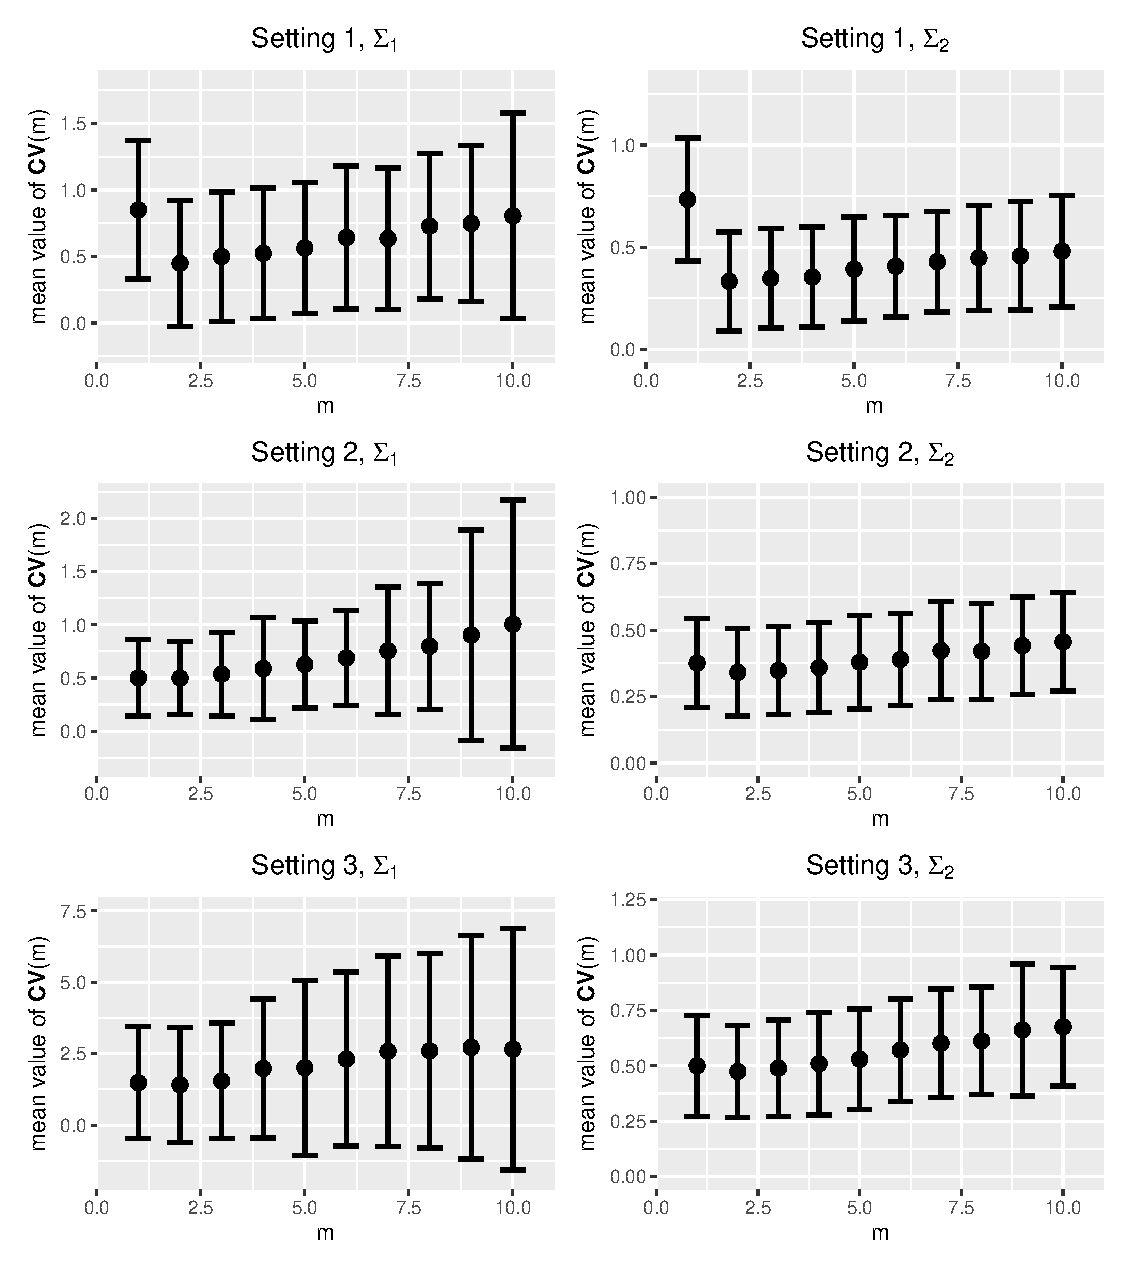
\includegraphics[width=1\textwidth,height=16cm]{cvtestnewnew.eps}
\caption{\scriptsize{
{\color{blue}Dot graphs with error bars of the values of the CV function versus the nuisance parameter $m$ in Settings 1--3 for  $n=100$, $\delta=0$, $\Sigma_{u}=\Sigma_1$ or $\Sigma_2$.}}}
\end{figure}

\clearpage\pagebreak\newpage


\begin{table}
\centering{
\caption{\scriptsize{{\color{blue}{Frequencies of rejecting the null hypothesis in Setting 1 under different sample sizes and test levels with
$\mathcal{D}(\mathbf{Z},X)=3 \|X\|^2$ in Case 1, and $\mathcal{D}(\mathbf{Z},X)=1.5|Z_1-Z_2|\cdot \|X\|$ in Case 2.
$\mathcal{T}_n^{BE}$: the test for accurately observed data; $\mathcal{T}_n^{KN}$: the proposed test with known covariance matrix of the measurement error variable; $\mathcal{T}_n^{UN}$: the proposed test with unknown covariance matrix of the measurement error variable; $\mathcal{T}_n^{NA}$: the naive test.}}}}
\vspace{5pt}
\resizebox{\textwidth}{98mm}{
\begin{tabular}{cccccccccccccc}
\hline\hline
  &    &  {\color{blue}$\Sigma_{u}$}  &    \multicolumn{5}{c}{$n=100$}  &    &  \multicolumn{5}{c}{$n=200$} \\
\cline{4-8}\cline{10-14}
 &  {\color{blue}Test}  &  {\color{blue}$\delta_n$}  & 0  & 1  &  1.5& 2 & 2.5 & & 0  & 1  &  1.5  & 2&2.5  \\
\hline
 $\alpha=0.05$          & $\mathcal{T}_n^{BE}$               &                        &{\textbf{0.058}}  &0.944  &0.960  &0.962  &0.966  &&{\textbf{0.050}}  &0.990  &0.992  &0.996  &0.998\\
\cline{3-14}
\multirow{6}{*}{Case 1} & \multirow{2}{*}{$\mathcal{T}_n^{KN}$}  &$\Sigma_1$          &{\textbf{0.046}}  &0.348  &0.528  &0.650  &0.708  &&{\textbf{0.048}}  &0.506  &0.740  &0.852  &0.914\\
                        &                                           &$\Sigma_2$       &{\textbf{0.054}}  &0.526  &0.718  &0.808  &0.844  &&{\textbf{0.052}}  &0.760  &0.936  &0.952  &0.972\\
\cline{3-14}
                        & \multirow{2}{*}{$\mathcal{T}_n^{UN}$}&$\Sigma_1$            &{\textbf{0.060}}  &0.356  &0.512  &0.582  &0.712  &&{\textbf{0.052}}  &0.504  &0.730  &0.834  &0.910\\
                        &                                           &$\Sigma_2$       &{\textbf{0.048}}  &0.540  &0.750  &0.798  &0.860  &&{\textbf{0.050}}  &0.746  &0.876  &0.960  &0.978\\
\cline{3-14}
                        & \multirow{2}{*}{$\mathcal{T}_n^{NA}$}  &$\Sigma_1$          &{\textbf{0.196}}  &0.346  &0.528  &0.614  &0.676  &&{\textbf{0.292}}  &0.562  &0.800  &0.848  &0.894\\
                        &                                           &$\Sigma_2$       &{\textbf{0.096}}  &0.522  &0.666  &0.760  &0.856  &&{\textbf{0.136}}  &0.704  &0.906  &0.950  &0.962\\
\cline{2-14}
                        & $\mathcal{T}_n^{BE}$               &                        &{\textbf{0.064}}  &0.994  &0.996  &0.996  &0.998  &&{\textbf{0.046}}  &0.998  &1.000  &1.000  &1.000\\
\cline{3-14}
\multirow{6}{*}{Case 2} & \multirow{2}{*}{$\mathcal{T}_n^{KN}$}  &$\Sigma_1$          &{\textbf{0.048}}  &0.262  &0.420  &0.522  &0.606  &&{\textbf{0.044}}  &0.388  &0.618  &0.696  &0.794\\
                        &                                           &$\Sigma_2$       &{\textbf{0.050}}  &0.500  &0.712  &0.806  &0.834  &&{\textbf{0.054}}  &0.726  &0.866  &0.932  &0.966\\
\cline{3-14}
                        & \multirow{2}{*}{$\mathcal{T}_n^{UN}$}&$\Sigma_1$            &{\textbf{0.054}}  &0.262  &0.432  &0.528  &0.586  &&{\textbf{0.052}}  &0.370  &0.522  &0.734  &0.776\\
                        &                                           &$\Sigma_2$       &{\textbf{0.048}}  &0.524  &0.674  &0.778  &0.834  &&{\textbf{0.050}}  &0.698  &0.858  &0.956  &0.962\\
\cline{3-14}
                        & \multirow{2}{*}{$\mathcal{T}_n^{NA}$}  &$\Sigma_1$          &{\textbf{0.194}}  &0.234  &0.412  &0.442  &0.532  &&{\textbf{0.322}}  &0.390  &0.594  &0.718  &0.770\\
                        &                                           &$\Sigma_2$       &{\textbf{0.086}}  &0.400  &0.610  &0.710  &0.762  &&{\textbf{0.126}}  &0.582  &0.790  &0.900  &0.958\\
\hline
 $\alpha=0.10$          & $\mathcal{T}_n^{BE}$               &                        &{\textbf{0.102}}  &0.972  &0.984  &0.988  &0.990  &&{\textbf{0.096}}  &0.996  &0.998  &1.000  &1.000\\
\cline{3-14}
\multirow{6}{*}{Case 1} & \multirow{2}{*}{$\mathcal{T}_n^{KN}$}  &$\Sigma_1$          &{\textbf{0.106}}  &0.466  &0.600  &0.736  &0.790  &&{\textbf{0.096}}  &0.572  &0.808  &0.920  &0.944\\
                        &                                           &$\Sigma_2$       &{\textbf{0.102}}  &0.630  &0.820  &0.884  &0.922  &&{\textbf{0.108}}  &0.834  &0.930  &0.970  &0.986\\
\cline{3-14}
                        & \multirow{2}{*}{$\mathcal{T}_n^{UN}$}&$\Sigma_1$            &{\textbf{0.116}}  &0.448  &0.642  &0.706  &0.798  &&{\textbf{0.098}}  &0.564  &0.788  &0.906  &0.946\\
                        &                                           &$\Sigma_2$       &{\textbf{0.106}}  &0.644  &0.824  &0.906  &0.936  &&{\textbf{0.104}}  &0.834  &0.944  &0.972  &0.984\\
\cline{3-14}
                        & \multirow{2}{*}{$\mathcal{T}_n^{NA}$}  &$\Sigma_1$          &{\textbf{0.268}}  &0.514  &0.676  &0.720  &0.804  &&{\textbf{0.376}}  &0.670  &0.814  &0.918  &0.958\\
                        &                                           &$\Sigma_2$       &{\textbf{0.170}}  &0.672  &0.796  &0.904  &0.944  &&{\textbf{0.190}}  &0.812  &0.946  &0.980  &0.982\\
\cline{2-14}
                        & $\mathcal{T}_n^{BE}$               &                        &{\textbf{0.114}}  &0.996  &1.000  &1.000  &1.000  &&{\textbf{0.100}}  &1.000  &1.000  &1.000  &1.000\\
\cline{3-14}
\multirow{6}{*}{Case 2} & \multirow{2}{*}{$\mathcal{T}_n^{KN}$}  &$\Sigma_1$          &{\textbf{0.094}}  &0.390  &0.544  &0.582  &0.692  &&{\textbf{0.096}}  &0.486  &0.702  &0.798  &0.864\\
                        &                                           &$\Sigma_2$       &{\textbf{0.104}}  &0.626  &0.770  &0.812  &0.874  &&{\textbf{0.104}}  &0.764  &0.944  &0.952  &0.978\\
\cline{3-14}
                        & \multirow{2}{*}{$\mathcal{T}_n^{UN}$}&$\Sigma_1$            &{\textbf{0.098}}  &0.374  &0.490  &0.576  &0.628  &&{\textbf{0.104}}  &0.472  &0.668  &0.778  &0.876\\
                        &                                           &$\Sigma_2$       &{\textbf{0.114}}  &0.596  &0.758  &0.840  &0.872  &&{\textbf{0.100}}  &0.804  &0.912  &0.954  &0.972\\
\cline{3-14}
                        & \multirow{2}{*}{$\mathcal{T}_n^{NA}$}  &$\Sigma_1$          &{\textbf{0.286}}  &0.362  &0.490  &0.602  &0.606  &&{\textbf{0.388}}  &0.540  &0.648  &0.788  &0.844\\
                        &                                           &$\Sigma_2$       &{\textbf{0.154}}  &0.510  &0.722  &0.784  &0.868  &&{\textbf{0.224}}  &0.704  &0.896  &0.956  &0.960\\
\hline
\end{tabular}}}
\end{table}

%\clearpage\pagebreak\newpage
%
%
%\begin{table}
%\centering{
%\caption{\scriptsize{{\color{blue}{Frequencies of rejecting the null hypothesis in Setting 1 under different sample sizes and test levels with
%$\mathcal{D}(\mathbf{Z},X)=1.5 \|X\|^2$ in Case 1, and $\mathcal{D}(\mathbf{Z},X)=5\exp(-2Z_2/\pi)$ in Case 2.
%$\mathcal{T}_n^{BE}$: the test for accurately observed data; $\mathcal{T}_n^{KN}$: the proposed test with known covariance matrix of the measurement error variable; $\mathcal{T}_n^{UN}$: the proposed test with unknown covariance matrix of the measurement error variable; $\mathcal{T}_n^{NA}$: the naive test.}}}}
%\vspace{5pt}
%\resizebox{\textwidth}{98mm}{
%\begin{tabular}{cccccccccccccc}
%\hline\hline
%  &    &  {\color{blue}$\Sigma_{u}$}  &    \multicolumn{5}{c}{$n=100$}  &    &  \multicolumn{5}{c}{$n=200$} \\
%\cline{4-8}\cline{10-14}
% &  Method  &  {\color{blue}$\delta_n$}  & 0  & 1  &  1.5& 2 & 2.5 & & 0  & 1  &  1.5  & 2&2.5  \\
%\hline
% $\alpha=0.05$          & $\mathcal{T}_n^{BE}$               &                        &{\textbf{0.049}}  &0.799  &0.907  &0.924  &0.953  &&{\textbf{}}  &  &  &  &\\
%\cline{3-14}
%\multirow{6}{*}{Case 1} & \multirow{2}{*}{$\mathcal{T}_n^{KN}$}  &$\Sigma_1$          &{\textbf{}}  &  &  &  &  &&{\textbf{}}  &  &  &  &\\
%                        &                                           &$\Sigma_2$       &{\textbf{}}  &  &  &  &  &&{\textbf{}}  &  &  &  &\\
%\cline{3-14}
%                        & \multirow{2}{*}{$\mathcal{T}_n^{UN}$}&$\Sigma_1$            &{\textbf{}}  &  &  &  &  &&{\textbf{}}  &  &  &  &\\
%                        &                                           &$\Sigma_2$       &{\textbf{}}  &  &  &  &  &&{\textbf{}}  &  &  &  &\\
%\cline{3-14}
%                        & \multirow{2}{*}{$\mathcal{T}_n^{NA}$}  &$\Sigma_1$          &{\textbf{}}  &  &  &  &  &&{\textbf{}}  &  &  &  &\\
%                        &                                           &$\Sigma_2$       &{\textbf{}}  &  &  &  &  &&{\textbf{}}  &  &  &  &\\
%\cline{2-14}
%                        & $\mathcal{T}_n^{BE}$               &                        &{\textbf{}}  &  &  &  &  &&{\textbf{}}  &  &  &  &\\
%\cline{3-14}
%\multirow{6}{*}{Case 2} & \multirow{2}{*}{$\mathcal{T}_n^{KN}$}  &$\Sigma_1$          &{\textbf{}}  &  &  &  &  &&{\textbf{}}  &  &  &  &\\
%                        &                                           &$\Sigma_2$       &{\textbf{}}  &  &  &  &  &&{\textbf{}}  &  &  &  &\\
%\cline{3-14}
%                        & \multirow{2}{*}{$\mathcal{T}_n^{UN}$}&$\Sigma_1$            &{\textbf{}}  &  &  &  &  &&{\textbf{}}  &  &  &  &\\
%                        &                                           &$\Sigma_2$       &{\textbf{}}  &  &  &  &  &&{\textbf{}}  &  &  &  &\\
%\cline{3-14}
%                        & \multirow{2}{*}{$\mathcal{T}_n^{NA}$}  &$\Sigma_1$          &{\textbf{}}  &  &  &  &  &&{\textbf{}}  &  &  &  &\\
%                        &                                           &$\Sigma_2$       &{\textbf{}}  &  &  &  &  &&{\textbf{}}  &  &  &  &\\
%\hline
% $\alpha=0.10$          & $\mathcal{T}_n^{BE}$               &                        &{\textbf{}}  &  &  &  &  &&{\textbf{}}  &  &  &  &\\
%\cline{3-14}
%\multirow{6}{*}{Case 1} & \multirow{2}{*}{$\mathcal{T}_n^{KN}$}  &$\Sigma_1$          &{\textbf{}}  &  &  &  &  &&{\textbf{}}  &  &  &  &\\
%                        &                                           &$\Sigma_2$       &{\textbf{}}  &  &  &  &  &&{\textbf{}}  &  &  &  &\\
%\cline{3-14}
%                        & \multirow{2}{*}{$\mathcal{T}_n^{UN}$}&$\Sigma_1$            &{\textbf{}}  &  &  &  &  &&{\textbf{}}  &  &  &  &\\
%                        &                                           &$\Sigma_2$       &{\textbf{}}  &  &  &  &  &&{\textbf{}}  &  &  &  &\\
%\cline{3-14}
%                        & \multirow{2}{*}{$\mathcal{T}_n^{NA}$}  &$\Sigma_1$          &{\textbf{}}  &  &  &  &  &&{\textbf{}}  &  &  &  &\\
%                        &                                           &$\Sigma_2$       &{\textbf{}}  &  &  &  &  &&{\textbf{}}  &  &  &  &\\
%\cline{2-14}
%                        & $\mathcal{T}_n^{BE}$               &                        &{\textbf{}}  &  &  &  &  &&{\textbf{}}  &  &  &  &\\
%\cline{3-14}
%\multirow{6}{*}{Case 2} & \multirow{2}{*}{$\mathcal{T}_n^{KN}$}  &$\Sigma_1$          &{\textbf{}}  &  &  &  &  &&{\textbf{}}  &  &  &  &\\
%                        &                                           &$\Sigma_2$       &{\textbf{}}  &  &  &  &  &&{\textbf{}}  &  &  &  &\\
%\cline{3-14}
%                        & \multirow{2}{*}{$\mathcal{T}_n^{UN}$}&$\Sigma_1$            &{\textbf{}}  &  &  &  &  &&{\textbf{}}  &  &  &  &\\
%                        &                                           &$\Sigma_2$       &{\textbf{}}  &  &  &  &  &&{\textbf{}}  &  &  &  &\\
%\cline{3-14}
%                        & \multirow{2}{*}{$\mathcal{T}_n^{NA}$}  &$\Sigma_1$          &{\textbf{}}  &  &  &  &  &&{\textbf{}}  &  &  &  &\\
%                        &                                           &$\Sigma_2$       &{\textbf{}}  &  &  &  &  &&{\textbf{}}  &  &  &  &\\
%\hline
%\end{tabular}}}
%\end{table}

\clearpage\pagebreak\newpage


%\begin{table}
%\centering{
%\caption{\scriptsize{{\color{blue}{Frequencies of rejecting the null hypothesis in Setting 1 under different sample sizes and test levels with
%$\mathcal{D}(\mathbf{Z},X)=1.5 \|X\|^2$ in Case 1, and $\mathcal{D}(\mathbf{Z},X)=5\exp(-2Z_2/\pi)$ in Case 2.
%$\mathcal{T}_n^{BE}$: the test for accurately observed data; $\mathcal{T}_n^{KN}$: the proposed test with known covariance matrix of the measurement error variable; $\mathcal{T}_n^{UN}$: the proposed test with unknown covariance matrix of the measurement error variable; $\mathcal{T}_n^{NA}$: the naive test.}}}}
%\vspace{5pt}
%\resizebox{\textwidth}{98mm}{
%\begin{tabular}{cccccccccccccc}
%\hline\hline
%  &    &  {\color{blue}$\Sigma_{u}$}  &    \multicolumn{5}{c}{$n=100$}  &    &  \multicolumn{5}{c}{$n=200$} \\
%\cline{4-8}\cline{10-14}
% &  Method  &  {\color{blue}$\delta_n$}  & 0  & 1  &  1.5& 2 & 2.5 & & 0  & 1  &  1.5  & 2&2.5  \\
%\hline
% $\alpha=0.05$          & $\mathcal{T}_n^{BE}$               &                        &{\textbf{0.052}}  &0.972  &0.986  &0.992  &0.996  &&{\textbf{0.046}}  &1.000  &1.000  &1.000  &1.000\\
%\cline{3-14}
%\multirow{6}{*}{Case 1} & \multirow{2}{*}{$\mathcal{T}_n^{KN}$}  &$\Sigma_1$          &{\textbf{0.056}}  &0.222  &0.386  &0.626  &0.716  &&{\textbf{0.044}}  &0.330  &0.700  &0.892  &0.954\\
%                        &                                           &$\Sigma_2$       &{\textbf{0.046}}  &0.368  &0.674  &0.832  &0.900  &&{\textbf{0.052}}  &0.656  &0.930  &0.988  &0.996\\
%\cline{3-14}
%                        & \multirow{2}{*}{$\mathcal{T}_n^{UN}$}&$\Sigma_1$            &{\textbf{0.064}}  &0.218  &0.396  &0.584  &0.748  &&{\textbf{0.056}}  &0.376  &0.720  &0.858  &0.956\\
%                        &                                           &$\Sigma_2$       &{\textbf{0.058}}  &0.380  &0.646  &0.842  &0.906  &&{\textbf{0.054}}  &0.676  &0.932  &0.982  &0.994\\
%\cline{3-14}
%                        & \multirow{2}{*}{$\mathcal{T}_n^{NA}$}  &$\Sigma_1$          &{\textbf{0.370}}  &0.418  &0.556  &0.692  &0.772  &&{\textbf{0.706}}  &0.802  &0.912  &0.960  &0.990\\
%                        &                                           &$\Sigma_2$       &{\textbf{0.116}}  &0.390  &0.648  &0.798  &0.884  &&{\textbf{0.272}}  &0.722  &0.952  &0.982  &0.998\\
%\cline{2-14}
%                        & $\mathcal{T}_n^{BE}$               &                        &{\textbf{0.046}}  &0.852  &0.884  &0.896  &0.902  &&{\textbf{0.050}}  &0.996  &0.998  &1.000  &1.000\\
%\cline{3-14}
%\multirow{6}{*}{Case 2} & \multirow{2}{*}{$\mathcal{T}_n^{KN}$}  &$\Sigma_1$          &{\textbf{0.060}}  &0.200  &0.344  &0.424  &0.478  &&{\textbf{0.046}}  &0.530  &0.672  &0.782  &0.836\\
%                        &                                           &$\Sigma_2$       &{\textbf{0.054}}  &0.414  &0.540  &0.598  &0.626  &&{\textbf{0.048}}  &0.770  &0.888  &0.946  &0.952\\
%\cline{3-14}
%                        & \multirow{2}{*}{$\mathcal{T}_n^{UN}$}&$\Sigma_1$            &{\textbf{0.060}}  &0.230  &0.332  &0.428  &0.486  &&{\textbf{0.056}}  &0.496  &0.656  &0.754  &0.822\\
%                        &                                           &$\Sigma_2$       &{\textbf{0.046}}  &0.384  &0.496  &0.620  &0.666  &&{\textbf{0.050}}  &0.734  &0.860  &0.932  &0.958\\
%\cline{3-14}
%                        & \multirow{2}{*}{$\mathcal{T}_n^{NA}$}  &$\Sigma_1$          &{\textbf{0.344}}  &0.982  &0.988  &0.990  &0.994  &&{\textbf{0.710}}  &1.000  &1.000  &1.000  &1.000\\
%                        &                                           &$\Sigma_2$       &{\textbf{0.158}}  &0.944  &0.962  &0.964  &0.966  &&{\textbf{0.296}}  &0.998  &1.000  &1.000  &1.000\\
%\hline
% $\alpha=0.10$          & $\mathcal{T}_n^{BE}$               &                        &{\textbf{0.096}}  &0.982  &0.990  &0.996  &1.000  &&{\textbf{0.102}}  &1.000  &1.000  &1.000  &1.000\\
%\cline{3-14}
%\multirow{6}{*}{Case 1} & \multirow{2}{*}{$\mathcal{T}_n^{KN}$}  &$\Sigma_1$          &{\textbf{0.112}}  &0.262  &0.450  &0.644  &0.784  &&{\textbf{0.088}}  &0.470  &0.764  &0.926  &0.980\\
%                        &                                           &$\Sigma_2$       &{\textbf{0.096}}  &0.460  &0.734  &0.890  &0.952  &&{\textbf{0.102}}  &0.760  &0.956  &0.990  &0.998\\
%\cline{3-14}
%                        & \multirow{2}{*}{$\mathcal{T}_n^{UN}$}&$\Sigma_1$            &{\textbf{0.110}}  &0.272  &0.534  &0.622  &0.770  &&{\textbf{0.094}}  &0.432  &0.766  &0.924  &0.972\\
%                        &                                           &$\Sigma_2$       &{\textbf{0.108}}  &0.490  &0.718  &0.862  &0.952  &&{\textbf{0.100}}  &0.692  &0.936  &0.990  &0.998\\
%\cline{3-14}
%                        & \multirow{2}{*}{$\mathcal{T}_n^{NA}$}  &$\Sigma_1$          &{\textbf{0.472}}  &0.536  &0.720  &0.788  &0.888  &&\boxed{{\textbf{0.806}}}  &0.884  &0.962  &0.982  &0.990\\
%                        &                                           &$\Sigma_2$       &{\textbf{0.210}}  &0.430  &0.736  &0.888  &0.936  &&{\textbf{0.382}}  &0.838  &0.956  &0.998  &1.000\\
%\cline{2-14}
%                        & $\mathcal{T}_n^{BE}$               &                        &{\textbf{0.106}}  &0.914  &0.916  &0.952  &0.956  &&{\textbf{0.104}}  &0.998  &0.998  &1.000  &1.000\\
%\cline{3-14}
%\multirow{6}{*}{Case 2} & \multirow{2}{*}{$\mathcal{T}_n^{KN}$}  &$\Sigma_1$          &{\textbf{0.112}}  &0.348  &0.410  &0.502  &0.544  &&{\textbf{0.096}}  &0.554  &0.720  &0.846  &0.868\\
%                        &                                           &$\Sigma_2$       &{\textbf{0.106}}  &0.458  &0.636  &0.670  &0.756  &&{\textbf{0.102}}  &0.812  &0.932  &0.960  &0.976\\
%\cline{3-14}
%                        & \multirow{2}{*}{$\mathcal{T}_n^{UN}$}&$\Sigma_1$            &{\textbf{0.106}}  &0.306  &0.440  &0.506  &0.560  &&{\textbf{0.098}}  &0.566  &0.734  &0.810  &0.862\\
%                        &                                           &$\Sigma_2$       &{\textbf{0.096}}  &0.468  &0.608  &0.702  &0.762  &&{\textbf{0.100}}  &0.846  &0.934  &0.944  &0.974\\
%\cline{3-14}
%                        & \multirow{2}{*}{$\mathcal{T}_n^{NA}$}  &$\Sigma_1$          &{\textbf{0.456}}  &0.994  &0.994  &0.996  &1.000  &&\boxed{{\textbf{0.782}}}  &1.000  &1.000  &1.000  &1.000\\
%                        &                                           &$\Sigma_2$       &{\textbf{0.190}}  &0.968  &0.980  &0.988  &0.990  &&{\textbf{0.352}}  &1.000  &1.000  &1.000  &1.000\\
%\hline
%\end{tabular}}}
%\end{table}


%\begin{figure}
%\centering
%\includegraphics[width=1\textwidth,height=16cm]{s1c1a5.eps}
%\caption{\scriptsize{
%{\color{blue}Frequencies of rejecting the null hypothesis in Setting 1 and Case 1 ($\mathcal{D}(\mathbf{Z},X)=1.5 \|X\|^2$) under different sample sizes and choices of $\Sigma_u$ with test level $\alpha=0.05$.}}}
%\end{figure}

\clearpage\pagebreak\newpage

%\begin{table}
%\centering{
%\caption{\scriptsize{Frequencies of rejecting the null hypothesis in Setting 1 under different sample sizes and test levels. $\mathcal{T}_n^{BE}$: the test for accurately observed data; $\mathcal{T}_n^{KN}$: the proposed test with known covariance matrix of the measurement error variable; $\mathcal{T}_n^{UN}$: the proposed test with unknown covariance matrix of the measurement error variable; $\mathcal{T}_n^{NA}$: the naive test.}}
%\vspace{5pt}
%\resizebox{\textwidth}{98mm}{
%\begin{tabular}{cccccccccccccc}
%\hline\hline
%  &    &  $\Sigma_{uu}$  &    \multicolumn{5}{c}{$n=100$}  &    &  \multicolumn{5}{c}{$n=200$} \\
%\cline{4-8}\cline{10-14}
% &  Method  &  $\delta$  & 0  & 1  &  1.5& 2 & 2.5 & & 0  & 1  &  1.5  & 2&2.5  \\
%\hline
% $\alpha=0.05$         & $\mathcal{T}_n^{BE}$               &          &0.054  &0.748  &0.930  &0.990  &0.994  &&0.052  &0.978  &0.998  &1.000  &1.000\\
%\cline{3-14}
%\multirow{6}{*}{Case 1}& \multirow{2}{*}{$\mathcal{T}_n^{KN}$}  &$\Sigma_1$&0.040  &0.110  &0.340  &0.516  &0.754  &&0.058  &0.200  &0.596  &0.888  &0.956\\
%                       &                                           &$\Sigma_2$&0.046  &0.240  &0.544  &0.826  &0.920  &&0.052  &0.406  &0.856  &0.974  &0.994\\
%\cline{3-14}
%                       & \multirow{2}{*}{$\mathcal{T}_n^{UN}$}&$\Sigma_1$&0.040  &0.132  &0.336  &0.606  &0.760  &&0.044  &0.184  &0.592  &0.858  &0.984\\
%                       &                                           &$\Sigma_2$&0.046  &0.224  &0.566  &0.822  &0.922  &&0.050  &0.400  &0.858  &0.984  &0.998\\
%\cline{3-14}
%                       & \multirow{2}{*}{$\mathcal{T}_n^{NA}$}  &$\Sigma_1$&0.128  &0.226  &0.484  &0.730  &0.838  &&0.160  &0.480  &0.814  &0.960  &0.988\\
%                       &                                           &$\Sigma_2$&0.068  &0.280  &0.608  &0.788  &0.928  &&0.086  &0.560  &0.894  &0.992  &0.998\\
%\cline{2-14}
%                       & $\mathcal{T}_n^{BE}$               &          &0.046  &0.802  &0.934  &0.958  &0.962  &&0.048  &0.972  &0.992  &0.992  &0.996\\
%\cline{3-14}
%\multirow{6}{*}{Case 2}& \multirow{2}{*}{$\mathcal{T}_n^{KN}$}  &$\Sigma_1$&0.060  &0.110  &0.204  &0.324  &0.450  &&0.044  &0.190  &0.404  &0.618  &0.736\\
%                       &                                           &$\Sigma_2$&0.042  &0.198  &0.396  &0.558  &0.670  &&0.046  &0.372  &0.674  &0.854  &0.928\\
%\cline{3-14}
%                       & \multirow{2}{*}{$\mathcal{T}_n^{UN}$}&$\Sigma_1$&0.040  &0.120  &0.208  &0.286  &0.436  &&0.054  &0.198  &0.402  &0.584  &0.754\\
%                       &                                           &$\Sigma_2$&0.046  &0.198  &0.424  &0.522  &0.680  &&0.048  &0.356  &0.684  &0.848  &0.926\\
%\cline{3-14}
%                       & \multirow{2}{*}{$\mathcal{T}_n^{NA}$}  &$\Sigma_1$&0.112  &0.048  &0.086  &0.088  &0.164  &&0.206  &0.054  &0.096  &0.156  &0.316\\
%                       &                                           &$\Sigma_2$&0.066  &0.072  &0.132  &0.238  &0.410  &&0.098  &0.108  &0.286  &0.514  &0.688\\
%\hline
% $\alpha=0.10$         & $\mathcal{T}_n^{BE}$               &          &0.092  &0.860  &0.982  &0.994  &0.998  &&0.106  &0.992  &1.000  &1.000  &1.000\\
%\cline{3-14}
%\multirow{6}{*}{Case 1}& \multirow{2}{*}{$\mathcal{T}_n^{KN}$}  &$\Sigma_1$&0.116  &0.194  &0.436  &0.656  &0.824  &&0.110  &0.336  &0.680  &0.906  &0.980\\
%                       &                                           &$\Sigma_2$&0.112  &0.316  &0.654  &0.878  &0.954  &&0.092  &0.522  &0.874  &0.988  &1.000\\
%\cline{3-14}
%                       & \multirow{2}{*}{$\mathcal{T}_n^{UN}$}&$\Sigma_1$&0.114  &0.190  &0.414  &0.670  &0.860  &&0.110  &0.302  &0.670  &0.916  &0.976\\
%                       &                                           &$\Sigma_2$&0.088  &0.304  &0.632  &0.872  &0.962  &&0.108  &0.510  &0.886  &0.990  &1.000\\
%\cline{3-14}
%                       & \multirow{2}{*}{$\mathcal{T}_n^{NA}$}  &$\Sigma_1$&0.190  &0.382  &0.568  &0.788  &0.938  &&0.288  &0.556  &0.858  &0.976  &1.000\\
%                       &                                           &$\Sigma_2$&0.112  &0.394  &0.728  &0.886  &0.954  &&0.166  &0.602  &0.908  &0.992  &1.000\\
%\cline{2-14}
%                       & $\mathcal{T}_n^{BE}$               &          &0.094  &0.884  &0.948  &0.972  &0.974  &&0.102  &0.978  &0.990  &0.996  &0.998\\
%\cline{3-14}
%\multirow{6}{*}{Case 2}& \multirow{2}{*}{$\mathcal{T}_n^{KN}$}  &$\Sigma_1$&0.114  &0.202  &0.316  &0.424  &0.562  &&0.108  &0.258  &0.512  &0.702  &0.778\\
%                       &                                           &$\Sigma_2$&0.092  &0.284  &0.512  &0.672  &0.800  &&0.098  &0.482  &0.762  &0.904  &0.948\\
%\cline{3-14}
%                       & \multirow{2}{*}{$\mathcal{T}_n^{UN}$}&$\Sigma_1$&0.114  &0.208  &0.262  &0.420  &0.500  &&0.110  &0.286  &0.434  &0.662  &0.830\\
%                       &                                           &$\Sigma_2$&0.106  &0.310  &0.446  &0.660  &0.772  &&0.100  &0.502  &0.746  &0.924  &0.972\\
%\cline{3-14}
%                       & \multirow{2}{*}{$\mathcal{T}_n^{NA}$}  &$\Sigma_1$&0.198  &0.098  &0.132  &0.164  &0.250  &&0.226  &0.116  &0.152  &0.262  &0.342\\
%                       &                                           &$\Sigma_2$&0.144  &0.124  &0.250  &0.360  &0.524  &&0.158  &0.170  &0.356  &0.616  &0.756\\
%\hline
%\end{tabular}}}
%\end{table}

%\begin{table}
%\centering{
%\caption{\scriptsize{Frequencies of rejecting the null hypothesis in Setting 2 under different sample sizes and test levels. $\mathcal{T}_n^{BE}$: the test for accurately observed data; $\mathcal{T}_n^{KN}$: the proposed test with known covariance matrix of the measurement error variable; $\mathcal{T}_n^{UN}$: the proposed test with unknown covariance matrix of the measurement error variable; $\mathcal{T}_n^{NA}$: the naive test.}}
%\vspace{5pt}
%\resizebox{\textwidth}{98mm}{
%\begin{tabular}{cccccccccccccc}
%\hline\hline
%  &    &  $\Sigma_{uu}$  &    \multicolumn{5}{c}{$n=100$}  &    &  \multicolumn{5}{c}{$n=200$} \\
%\cline{4-8}\cline{10-14}
% &  Method  &  $\delta$  & 0  & 1  &  1.5& 2 & 2.5 & & 0  & 1  &  1.5  & 2&2.5  \\
%\hline
% $\alpha=0.05$          & $\mathcal{T}_n^{BE}$               &                    &0.054  &0.996  &1.000  &1.000  &1.000  &&0.052  &1.000  &1.000  &1.000  &1.000\\
%\cline{3-14}
%\multirow{6}{*}{Case 1} & \multirow{2}{*}{$\mathcal{T}_n^{KN}$}  &$\Sigma_1$          &0.042  &0.306  &0.634  &0.764  &0.872  &&0.056  &0.566  &0.866  &0.964  &0.994\\
%                        &                                           &$\Sigma_2$          &0.054  &0.584  &0.872  &0.956  &0.968  &&0.048  &0.904  &0.984  &1.000  &1.000\\
%\cline{3-14}
%                        & \multirow{2}{*}{$\mathcal{T}_n^{UN}$}&$\Sigma_1$          &0.058  &0.276  &0.580  &0.752  &0.864  &&0.054  &0.608  &0.900  &0.982  &0.996\\
%                        &                                           &$\Sigma_2$          &0.056  &0.570  &0.814  &0.946  &0.966  &&0.050  &0.864  &0.990  &1.000  &1.000\\
%\cline{3-14}
%                        & \multirow{2}{*}{$\mathcal{T}_n^{NA}$}  &$\Sigma_1$&0.180  &0.852  &0.978  &0.996  &0.998  &&0.290  &0.994  &1.000  &1.000  &1.000\\
%                        &                                           &$\Sigma_2$&0.078  &0.890  &0.986  &0.998  &0.998  &&0.130  &0.998  &1.000  &1.000  &1.000\\
%\cline{2-14}
%                        & $\mathcal{T}_n^{BE}$               &                    &0.044  &0.940  &0.996  &1.000  &1.000  &&0.048  &0.996  &1.000  &1.000  &1.000\\
%\cline{3-14}
%\multirow{6}{*}{Case 2} & \multirow{2}{*}{$\mathcal{T}_n^{KN}$}  &$\Sigma_1$          &0.062  &0.226  &0.558  &0.888  &0.960  &&0.044  &0.444  &0.862  &0.992  &0.994\\
%                        &                                           &$\Sigma_2$          &0.040  &0.444  &0.898  &0.998  &1.000  &&0.050  &0.758  &0.984  &1.000  &1.000\\
%\cline{3-14}
%                        & \multirow{2}{*}{$\mathcal{T}_n^{UN}$}&$\Sigma_1$          &0.058  &0.238  &0.562  &0.890  &0.970  &&0.056  &0.442  &0.906  &0.998  &1.000\\
%                        &                                           &$\Sigma_2$          &0.046  &0.430  &0.844  &0.968  &0.998  &&0.052  &0.776  &0.988  &1.000  &1.000\\
%\cline{3-14}
%                        & \multirow{2}{*}{$\mathcal{T}_n^{NA}$}  &$\Sigma_1$&0.192  &0.180  &0.494  &0.794  &0.936  &&0.272  &0.344  &0.828  &0.986  &0.998\\
%                        &                                           &$\Sigma_2$&0.088  &0.300  &0.732  &0.934  &0.992  &&0.134  &0.596  &0.968  &1.000  &1.000\\
%\hline
% $\alpha=0.10$          & $\mathcal{T}_n^{BE}$               &                    &0.106  &0.998  &1.000  &1.000  &1.000  &&0.096  &1.000  &1.000  &1.000  &1.000\\
%\cline{3-14}
%\multirow{6}{*}{Case 1} & \multirow{2}{*}{$\mathcal{T}_n^{KN}$}  &$\Sigma_1$          &0.110  &0.430  &0.652  &0.840  &0.894  &&0.108  &0.666  &0.918  &0.984  &0.998\\
%                        &                                           &$\Sigma_2$          &0.106  &0.690  &0.894  &0.972  &0.982  &&0.102  &0.942  &0.998  &1.000  &1.000\\
%\cline{3-14}
%                        & \multirow{2}{*}{$\mathcal{T}_n^{UN}$}&$\Sigma_1$          &0.116  &0.380  &0.636  &0.856  &0.898  &&0.088  &0.668  &0.924  &0.984  &1.000\\
%                        &                                           &$\Sigma_2$          &0.112  &0.640  &0.918  &0.960  &0.982  &&0.098  &0.930  &0.998  &1.000  &1.000\\
%\cline{3-14}
%                        & \multirow{2}{*}{$\mathcal{T}_n^{NA}$}  &$\Sigma_1$&0.248  &0.916  &0.992  &0.996  &1.000  &&0.390  &0.996  &1.000  &1.000  &1.000\\
%                        &                                           &$\Sigma_2$&0.168  &0.926  &0.994  &0.998  &1.000  &&0.190  &0.998  &1.000  &1.000  &1.000\\
%\cline{2-14}
%                        & $\mathcal{T}_n^{BE}$               &                    &0.106  &0.956  &1.000  &1.000  &1.000  &&0.096  &1.000  &1.000  &1.000  &1.000\\
%\cline{3-14}
%\multirow{6}{*}{Case 2} & \multirow{2}{*}{$\mathcal{T}_n^{KN}$}  &$\Sigma_1$          &0.114  &0.310  &0.674  &0.930  &0.988  &&0.090  &0.540  &0.946  &1.000  &1.000\\
%                        &                                           &$\Sigma_2$          &0.112  &0.460  &0.908  &0.988  &0.998  &&0.096  &0.814  &0.995  &1.000  &1.000\\
%\cline{3-14}
%                        & \multirow{2}{*}{$\mathcal{T}_n^{UN}$}&$\Sigma_1$          &0.112  &0.296  &0.650  &0.938  &0.980  &&0.088  &0.556  &0.960  &1.000  &1.000\\
%                        &                                           &$\Sigma_2$          &0.092  &0.504  &0.884  &0.984  &0.998  &&0.104  &0.820  &0.998  &1.000  &1.000\\
%\cline{3-14}
%                        & \multirow{2}{*}{$\mathcal{T}_n^{NA}$}  &$\Sigma_1$&0.220  &0.252  &0.624  &0.868  &0.982  &&0.408  &0.500  &0.868  &0.998  &1.000\\
%                        &                                           &$\Sigma_2$&0.126  &0.318  &0.784  &0.968  &0.996  &&0.188  &0.642  &0.980  &1.000  &1.000\\
%\hline
%\end{tabular}}}
%\end{table}

\begin{table}
\centering{
\caption{\scriptsize{{\color{blue}Frequencies of rejecting the null hypothesis in Setting 2 under different sample sizes and test levels with
$\mathcal{D}(\mathbf{Z},X)=1.2 \big(\exp(\Vert X \Vert)-1\big) $ in Case 1, and $\mathcal{D}(\mathbf{Z},X)=2 \exp(|Z_4-1|)/3$ in Case 2.
The meanings of  $\mathcal{T}_n^{BE}$, $\mathcal{T}_n^{KN}$,  $\mathcal{T}_n^{UN}$ and $\mathcal{T}_n^{NA}$ are the same as those in Table 1.}}}
\vspace{5pt}
\resizebox{\textwidth}{98mm}{
\begin{tabular}{cccccccccccccc}
\hline\hline
  &    &  {\color{blue}$\Sigma_{u}$}  &    \multicolumn{5}{c}{$n=100$}  &    &  \multicolumn{5}{c}{$n=200$} \\
\cline{4-8}\cline{10-14}
 &  {\color{blue}Test}  &  {\color{blue}$\delta_n$}  & 0  & 1  &  1.5& 2 & 2.5 & & 0  & 1  &  1.5  & 2&2.5  \\
\hline
 $\alpha=0.05$          & $\mathcal{T}_n^{BE}$               &                        &{\textbf{0.046}}  &0.980  &0.988  &0.994  &0.998  &&{\textbf{0.048}}  &0.998  &1.000  &1.000  &1.000\\
\cline{3-14}
\multirow{6}{*}{Case 1} & \multirow{2}{*}{$\mathcal{T}_n^{KN}$}  &$\Sigma_1$          &{\textbf{0.060}}  &0.214  &0.520  &0.672  &0.734  &&{\textbf{0.054}}  &0.542  &0.854  &0.940  &0.974\\
                        &                                           &$\Sigma_2$       &{\textbf{0.056}}  &0.492  &0.790  &0.898  &0.922  &&{\textbf{0.052}}  &0.842  &0.986  &0.996  &1.000\\
\cline{3-14}
                        & \multirow{2}{*}{$\mathcal{T}_n^{UN}$}&$\Sigma_1$            &{\textbf{0.040}}  &0.264  &0.496  &0.652  &0.772  &&{\textbf{0.042}}  &0.524  &0.828  &0.926  &0.984\\
                        &                                           &$\Sigma_2$       &{\textbf{0.046}}  &0.528  &0.798  &0.884  &0.938  &&{\textbf{0.052}}  &0.802  &0.990  &0.992  &0.998\\
\cline{3-14}
                        & \multirow{2}{*}{$\mathcal{T}_n^{NA}$}  &$\Sigma_1$          &{\textbf{0.198}}  &0.760  &0.918  &0.962  &0.968  &&{\textbf{0.402}}  &0.992  &0.998  &1.000  &1.000\\
                        &                                           &$\Sigma_2$       &{\textbf{0.096}}  &0.772  &0.948  &0.970  &0.982  &&{\textbf{0.136}}  &0.986  &0.998  &0.998  &1.000\\
\cline{2-14}
                        & $\mathcal{T}_n^{BE}$               &                        &{\textbf{0.044}}  &0.990  &1.000  &1.000  &1.000  &&{\textbf{0.050}}  &1.000  &1.000  &1.000  &1.000\\
\cline{3-14}
\multirow{6}{*}{Case 2} & \multirow{2}{*}{$\mathcal{T}_n^{KN}$}  &$\Sigma_1$          &{\textbf{0.038}}  &0.326  &0.646  &0.858  &0.934  &&{\textbf{0.058}}  &0.666  &0.944  &0.998  &1.000\\
                        &                                           &$\Sigma_2$       &{\textbf{0.040}}  &0.620  &0.896  &0.982  &0.994  &&{\textbf{0.054}}  &0.948  &0.998  &1.000  &1.000\\
\cline{3-14}
                        & \multirow{2}{*}{$\mathcal{T}_n^{UN}$}&$\Sigma_1$            &{\textbf{0.060}}  &0.280  &0.614  &0.834  &0.896  &&{\textbf{0.042}}  &0.648  &0.952  &1.000  &1.000\\
                        &                                           &$\Sigma_2$       &{\textbf{0.056}}  &0.586  &0.894  &0.986  &0.998  &&{\textbf{0.052}}  &0.940  &1.000  &1.000  &1.000\\
\cline{3-14}
                        & \multirow{2}{*}{$\mathcal{T}_n^{NA}$}  &$\Sigma_1$          &{\textbf{0.204}}  &0.662  &0.922  &0.990  &0.996  &&{\textbf{0.442}} &0.974  &1.000  &1.000  &1.000\\
                        &                                           &$\Sigma_2$       &{\textbf{0.110}}  &0.750  &0.970  &0.994  &0.998  &&{\textbf{0.174}} &0.980  &1.000  &1.000  &1.000\\
\hline
 $\alpha=0.10$          & $\mathcal{T}_n^{BE}$               &                        &{\textbf{0.108}}  &0.990  &0.996  &0.998  &1.000  &&{\textbf{0.100}}  &1.000  &1.000  &1.000  &1.000\\
\cline{3-14}
\multirow{6}{*}{Case 1} & \multirow{2}{*}{$\mathcal{T}_n^{KN}$}  &$\Sigma_1$          &{\textbf{0.114}}  &0.348  &0.598  &0.750  &0.864  &&{\textbf{0.108}}  &0.670  &0.834  &0.968  &0.984\\
                        &                                           &$\Sigma_2$       &{\textbf{0.092}}  &0.630  &0.824  &0.938  &0.970  &&{\textbf{0.104}}  &0.894  &0.994  &0.996  &1.000\\
\cline{3-14}
                        & \multirow{2}{*}{$\mathcal{T}_n^{UN}$}&$\Sigma_1$            &{\textbf{0.090}}  &0.390  &0.586  &0.716  &0.806  &&{\textbf{0.092}}  &0.626  &0.890  &0.972  &0.982\\
                        &                                           &$\Sigma_2$       &{\textbf{0.106}}  &0.584  &0.848  &0.924  &0.950  &&{\textbf{0.098}}  &0.866  &0.994  &0.998  &1.000\\
\cline{3-14}
                        & \multirow{2}{*}{$\mathcal{T}_n^{NA}$}  &$\Sigma_1$          &{\textbf{0.250}}  &0.860  &0.942  &0.978  &0.990  &&{\boxed{\textbf{0.466}}}  &0.988  &0.998  &1.000  &1.000\\
                        &                                           &$\Sigma_2$       &{\textbf{0.178}}  &0.876  &0.954  &0.976  &0.998  &&{\textbf{0.252}}  &0.988  &0.998  &1.000  &1.000\\
\cline{2-14}
                        & $\mathcal{T}_n^{BE}$               &                        &{\textbf{0.106}}  &0.996  &1.000  &1.000  &1.000  &&{\textbf{0.104}}  &1.000  &1.000  &1.000  &1.000\\
\cline{3-14}
\multirow{6}{*}{Case 2} & \multirow{2}{*}{$\mathcal{T}_n^{KN}$}  &$\Sigma_1$          &{\textbf{0.108}}  &0.366  &0.698  &0.894  &0.950  &&{\textbf{0.094}}  &0.762  &0.974  &1.000  &1.000\\
                        &                                           &$\Sigma_2$       &{\textbf{0.106}}  &0.694  &0.932  &0.992  &0.996  &&{\textbf{0.102}}  &0.962  &1.000  &1.000  &1.000\\
\cline{3-14}
                        & \multirow{2}{*}{$\mathcal{T}_n^{UN}$}&$\Sigma_1$            &{\textbf{0.112}}  &0.388  &0.698  &0.896  &0.942  &&{\textbf{0.108}}  &0.720  &0.972  &0.998  &1.000\\
                        &                                           &$\Sigma_2$       &{\textbf{0.108}}  &0.700  &0.958  &0.992  &0.994  &&{\textbf{0.106}}  &0.968  &1.000  &1.000  &1.000\\
\cline{3-14}
                        & \multirow{2}{*}{$\mathcal{T}_n^{NA}$}  &$\Sigma_1$          &{\textbf{0.280}}  &0.786  &0.950  &0.992  &1.000  &&{\boxed{\textbf{0.470}}}  &0.982  &1.000  &1.000  &1.000\\
                        &                                           &$\Sigma_2$       &{\textbf{0.154}}  &0.836  &0.974  &1.000  &1.000  &&{\textbf{0.226}}  &0.998  &1.000  &1.000  &1.000\\
\hline
\end{tabular}}}
\end{table}

%\begin{figure}
%\centering
%\includegraphics[width=1\textwidth,height=16cm]{s2c1a5.eps}
%\caption{\scriptsize{
%{\color{blue}Frequencies of rejecting the null hypothesis in Setting 2 and Case 1 ($\mathcal{D}(\mathbf{Z},X)=1.2 \big(\exp(\Vert X \Vert)-1\big) $) under different sample sizes and choices of $\Sigma_u$ with test level $\alpha=0.05$.}}}
%\end{figure}

\clearpage\pagebreak\newpage

%\begin{table}
%\centering{
%\caption{\scriptsize{{\color{red}{Frequencies of rejecting the null hypothesis in Setting 4 under different sample sizes and test levels. $\mathcal{T}_n^{BE}$: the test for accurately observed data; $\mathcal{T}_n^{KN}$: the proposed test with known covariance matrix of the measurement error variable; $\mathcal{T}_n^{UN}$: the proposed test with unknown covariance matrix of the measurement error variable; $\mathcal{T}_n^{NA}$: the naive test.}}}}
%\vspace{5pt}
%\resizebox{\textwidth}{98mm}{
%\begin{tabular}{cccccccccccccc}
%\hline\hline
%  &    &  $\Sigma_{uu}$  &    \multicolumn{5}{c}{$n=100$}  &    &  \multicolumn{5}{c}{$n=200$} \\
%\cline{4-8}\cline{10-14}
% &  Method  &  $\delta$  & 0  & 1  &  1.5& 2 & 2.5 & & 0  & 1  &  1.5  & 2&2.5  \\
%\hline
% $\alpha=0.05$          & $\mathcal{T}_n^{BE}$               &                        &0.056  &0.852  &0.952  &0.972  &0.980  &&0.046  &0.984  &0.992  &0.994  &0.998\\
%\cline{3-14}
%\multirow{6}{*}{Case 1} & \multirow{2}{*}{$\mathcal{T}_n^{KN}$}  &$\Sigma_1$          &0.056  &0.222  &0.386  &0.626  &0.716  &&0.044  &0.330  &0.700  &0.892  &0.954\\
%                        &                                           &$\Sigma_2$       &0.046  &0.368  &0.674  &0.832  &0.900  &&0.052  &0.656  &0.930  &0.988  &0.996\\
%\cline{3-14}
%                        & \multirow{2}{*}{$\mathcal{T}_n^{UN}$}&$\Sigma_1$            &0.064  &0.218  &0.396  &0.584  &0.748  &&0.056  &0.376  &0.720  &0.858  &0.956\\
%                        &                                           &$\Sigma_2$       &0.058  &0.380  &0.646  &0.842  &0.906  &&0.054  &0.676  &0.932  &0.982  &0.994\\
%\cline{3-14}
%                        & \multirow{2}{*}{$\mathcal{T}_n^{NA}$}  &$\Sigma_1$          &0.338  &0.588  &0.742  &0.872  &0.894  &&0.532  &0.844  &0.970  &0.972  &0.988\\
%                        &                                           &$\Sigma_2$       &0.116  &0.464  &0.702  &0.852  &0.874  &&0.246  &0.772  &0.944  &0.984  &0.986\\
%\cline{2-14}
%                        & $\mathcal{T}_n^{BE}$               &                        &0.042  &0.988  &0.990  &0.992  &0.996  &&0.044  &0.998  &1.000  &1.000  &1.000\\
%\cline{3-14}
%\multirow{6}{*}{Case 2} & \multirow{2}{*}{$\mathcal{T}_n^{KN}$}  &$\Sigma_1$          &0.060  &0.200  &0.344  &0.424  &0.478  &&0.046  &0.530  &0.672  &0.782  &0.836\\
%                        &                                           &$\Sigma_2$       &0.054  &0.414  &0.540  &0.598  &0.626  &&0.048  &0.770  &0.888  &0.946  &0.952\\
%\cline{3-14}
%                        & \multirow{2}{*}{$\mathcal{T}_n^{UN}$}&$\Sigma_1$            &0.060  &0.230  &0.332  &0.428  &0.486  &&0.056  &0.496  &0.656  &0.754  &0.822\\
%                        &                                           &$\Sigma_2$       &0.046  &0.384  &0.496  &0.620  &0.666  &&0.050  &0.734  &0.860  &0.932  &0.958\\
%\cline{3-14}
%                        & \multirow{2}{*}{$\mathcal{T}_n^{NA}$}  &$\Sigma_1$          &0.344  &0.988  &0.994  &0.998  &0.998  &&0.562  &0.994  &1.000  &1.000  &1.000\\
%                        &                                           &$\Sigma_2$       &0.142  &0.988  &0.990  &0.992  &0.996  &&0.220  &1.000  &1.000  &1.000  &1.000\\
%\hline
% $\alpha=0.10$          & $\mathcal{T}_n^{BE}$               &                        &0.088  &0.908  &0.980  &0.994  &0.996  &&0.106  &0.994  &0.998  &1.000  &1.000\\
%\cline{3-14}
%\multirow{6}{*}{Case 1} & \multirow{2}{*}{$\mathcal{T}_n^{KN}$}  &$\Sigma_1$          &0.112  &0.262  &0.450  &0.644  &0.784  &&0.088  &0.470  &0.764  &0.926  &0.980\\
%                        &                                           &$\Sigma_2$       &0.096  &0.460  &0.734  &0.890  &0.952  &&0.102  &0.760  &0.956  &0.990  &0.998\\
%\cline{3-14}
%                        & \multirow{2}{*}{$\mathcal{T}_n^{UN}$}&$\Sigma_1$            &0.110  &0.272  &0.534  &0.622  &0.770  &&0.094  &0.432  &0.766  &0.924  &0.972\\
%                        &                                           &$\Sigma_2$       &0.108  &0.490  &0.718  &0.862  &0.952  &&0.100  &0.692  &0.936  &0.990  &0.998\\
%\cline{3-14}
%                        & \multirow{2}{*}{$\mathcal{T}_n^{NA}$}  &$\Sigma_1$          &0.440  &0.742  &0.876  &0.888  &0.960  &&0.690  &0.928  &0.982  &0.994  &1.000\\
%                        &                                           &$\Sigma_2$       &0.250  &0.622  &0.824  &0.940  &0.966  &&0.336  &0.874  &0.984  &0.996  &1.000\\
%\cline{2-14}
%                        & $\mathcal{T}_n^{BE}$               &                        &0.094  &1.000  &1.000  &1.000  &1.000  &&0.100  &1.000  &1.000  &1.000  &1.000\\
%\cline{3-14}
%\multirow{6}{*}{Case 2} & \multirow{2}{*}{$\mathcal{T}_n^{KN}$}  &$\Sigma_1$          &0.112  &0.348  &0.410  &0.502  &0.544  &&0.096  &0.554  &0.720  &0.846  &0.868\\
%                        &                                           &$\Sigma_2$       &0.106  &0.458  &0.636  &0.670  &0.756  &&0.102  &0.812  &0.932  &0.960  &0.976\\
%\cline{3-14}
%                        & \multirow{2}{*}{$\mathcal{T}_n^{UN}$}&$\Sigma_1$            &0.106  &0.306  &0.440  &0.506  &0.560  &&0.098  &0.566  &0.734  &0.810  &0.862\\
%                        &                                           &$\Sigma_2$       &0.096  &0.468  &0.608  &0.702  &0.762  &&0.100  &0.846  &0.934  &0.944  &0.974\\
%\cline{3-14}
%                        & \multirow{2}{*}{$\mathcal{T}_n^{NA}$}  &$\Sigma_1$          &0.484  &1.000  &1.000  &1.000  &1.000  &&0.642  &1.000  &1.000  &1.000  &1.000\\
%                        &                                           &$\Sigma_2$       &0.238  &0.998  &1.000  &1.000  &1.000  &&0.356  &1.000  &1.000  &1.000  &1.000\\
%\hline
%\end{tabular}}}
%\end{table}

\clearpage\pagebreak\newpage

\begin{table}
\centering{
\caption{\scriptsize{{\color{blue}{Frequencies of rejecting the null hypothesis in Setting 3 under different sample sizes and test levels with
$\mathcal{D}(\mathbf{Z},X)=4 \log (1+ \|X\|^2) $ in Case 1, and $\mathcal{D}(\mathbf{Z},X)=Z_8^3/4$ in Case 2.
The meanings of  $\mathcal{T}_n^{BE}$, $\mathcal{T}_n^{KN}$,  $\mathcal{T}_n^{UN}$ and $\mathcal{T}_n^{NA}$ are the same as those in Table 1.}}}}
\vspace{5pt}
\resizebox{\textwidth}{98mm}{
\begin{tabular}{cccccccccccccc}
\hline\hline
  &    &  {\color{blue}$\Sigma_{u}$}  &    \multicolumn{5}{c}{$n=100$}  &    &  \multicolumn{5}{c}{$n=200$} \\
\cline{4-8}\cline{10-14}
 &  {\color{blue}Test}  &  {\color{blue}$\delta_n$}  & 0  & 1  &  1.5& 2 & 2.5 & & 0  & 1  &  1.5  & 2&2.5  \\
\hline
 $\alpha=0.05$          & $\mathcal{T}_n^{BE}$               &                        &{\textbf{0.044}}  &0.974  &0.998  &0.998  &1.000  &&{\textbf{0.052}}  &0.998  &1.000  &1.000  &1.000\\
\cline{3-14}
\multirow{6}{*}{Case 1} & \multirow{2}{*}{$\mathcal{T}_n^{KN}$}  &$\Sigma_1$          &{\textbf{0.052}}  &0.178  &0.366  &0.504  &0.584  &&{\textbf{0.048}}  &0.492  &0.796  &0.946  &0.968\\
                        &                                           &$\Sigma_2$       &{\textbf{0.044}}  &0.470  &0.766  &0.850  &0.926  &&{\textbf{0.054}}  &0.802  &0.974  &0.992  &0.996\\
\cline{3-14}
                        & \multirow{2}{*}{$\mathcal{T}_n^{UN}$}&$\Sigma_1$            &{\textbf{0.046}}  &0.188  &0.324  &0.432  &0.514  &&{\textbf{0.048}}  &0.480  &0.770  &0.892  &0.932\\
                        &                                           &$\Sigma_2$       &{\textbf{0.056}}  &0.460  &0.688  &0.864  &0.920  &&{\textbf{0.044}}  &0.806  &0.974  &0.982  &0.998\\
\cline{3-14}
                        & \multirow{2}{*}{$\mathcal{T}_n^{NA}$}  &$\Sigma_1$          &{\textbf{0.116}}  &0.656  &0.864  &0.930  &0.970  &&{\textbf{0.204}}  &0.916  &0.992  &0.998  &1.000\\
                        &                                           &$\Sigma_2$       &{\textbf{0.072}}  &0.730  &0.892  &0.968  &0.980  &&{\textbf{0.088}}  &0.958  &0.998  &1.000  &1.000\\
\cline{2-14}
                        & $\mathcal{T}_n^{BE}$               &                        &{\textbf{0.060}}  &0.910  &0.974  &0.982  &0.988  &&{\textbf{0.058}}  &0.998  &0.998  &1.000  &1.000\\
\cline{3-14}
\multirow{6}{*}{Case 2} & \multirow{2}{*}{$\mathcal{T}_n^{KN}$}  &$\Sigma_1$          &{\textbf{0.060}}  &0.240  &0.512  &0.732  &0.756  &&{\textbf{0.044}}  &0.612  &0.942  &0.986  &0.994\\
                        &                                           &$\Sigma_2$       &{\textbf{0.040}}  &0.524  &0.820  &0.898  &0.932  &&{\textbf{0.046}}  &0.876  &0.996  &0.996  &1.000\\
\cline{3-14}
                        & \multirow{2}{*}{$\mathcal{T}_n^{UN}$}&$\Sigma_1$            &{\textbf{0.048}}  &0.234  &0.450  &0.594  &0.668  &&{\textbf{0.058}}  &0.598  &0.934  &0.988  &0.996\\
                        &                                           &$\Sigma_2$       &{\textbf{0.060}}  &0.482  &0.792  &0.912  &0.922  &&{\textbf{0.052}}  &0.894  &0.996  &0.998  &1.000\\
\cline{3-14}
                        & \multirow{2}{*}{$\mathcal{T}_n^{NA}$}  &$\Sigma_1$          &{\textbf{0.118}}  &0.398  &0.776  &0.918  &0.960  &&{\textbf{0.184}}  &0.760  &0.998  &0.998  &1.000\\
                        &                                           &$\Sigma_2$       &{\textbf{0.066}}  &0.548  &0.866  &0.944  &0.956  &&{\textbf{0.096}}  &0.886  &0.998  &1.000  &1.000\\
\hline
$\alpha=0.10$          & $\mathcal{T}_n^{BE}$               &                         &{\textbf{0.104}}  &0.990  &0.998  &1.000  &1.000  &&{\textbf{0.092}}  &1.000  &1.000  &1.000  &1.000\\
\cline{3-14}
\multirow{6}{*}{Case 1} & \multirow{2}{*}{$\mathcal{T}_n^{KN}$}  &$\Sigma_1$          &{\textbf{0.112}}  &0.306  &0.416  &0.582  &0.666  &&{\textbf{0.104}}  &0.602  &0.862  &0.946  &0.990\\
                        &                                           &$\Sigma_2$       &{\textbf{0.096}}  &0.628  &0.826  &0.912  &0.940  &&{\textbf{0.102}}  &0.900  &0.984  &0.996  &1.000\\
\cline{3-14}
                        & \multirow{2}{*}{$\mathcal{T}_n^{UN}$}&$\Sigma_1$            &{\textbf{0.110}}  &0.282  &0.412  &0.510  &0.610  &&{\textbf{0.104}}  &0.534  &0.842  &0.936  &0.964\\
                        &                                           &$\Sigma_2$       &{\textbf{0.100}}  &0.580  &0.804  &0.900  &0.936  &&{\textbf{0.102}}  &0.886  &0.994  &1.000  &1.000\\
\cline{3-14}
                        & \multirow{2}{*}{$\mathcal{T}_n^{NA}$}  &$\Sigma_1$          &{\textbf{0.180}}  &0.758  &0.910  &0.970  &0.986  &&{\textbf{0.328}}  &0.958  &0.998  &1.000  &1.000\\
                        &                                           &$\Sigma_2$       &{\textbf{0.142}}  &0.788  &0.954  &0.984  &0.994  &&{\textbf{0.172}}  &0.970  &1.000  &1.000  &1.000\\
\cline{2-14}
 $\alpha=0.10$          & $\mathcal{T}_n^{BE}$               &                        &{\textbf{0.110}}  &0.968  &0.992  &0.992  &0.994  &&{\textbf{0.100}}  &0.998  &0.998  &1.000  &1.000\\
\cline{3-14}
\multirow{6}{*}{Case 2} & \multirow{2}{*}{$\mathcal{T}_n^{KN}$}  &$\Sigma_1$          &{\textbf{0.112}}  &0.318  &0.600  &0.776  &0.838  &&{\textbf{0.098}}  &0.698  &0.966  &0.992  &1.000\\
                        &                                           &$\Sigma_2$       &{\textbf{0.094}}  &0.610  &0.916  &0.948  &0.964  &&{\textbf{0.104}}  &0.946  &1.000  &1.000  &1.000\\
\cline{3-14}
                        & \multirow{2}{*}{$\mathcal{T}_n^{UN}$}&$\Sigma_1$            &{\textbf{0.110}}  &0.318  &0.564  &0.722  &0.770  &&{\textbf{0.094}}  &0.692  &0.966  &0.994  &1.000\\
                        &                                           &$\Sigma_2$       &{\textbf{0.112}}  &0.598  &0.854  &0.942  &0.974  &&{\textbf{0.096}}  &0.954  &0.998  &1.000  &1.000\\
\cline{3-14}
                        & \multirow{2}{*}{$\mathcal{T}_n^{NA}$}  &$\Sigma_1$          &{\textbf{0.188}}  &0.506  &0.830  &0.956  &0.974  &&{\textbf{0.284}}  &0.840  &0.992  &1.000  &1.000\\
                        &                                           &$\Sigma_2$       &{\textbf{0.142}}  &0.694  &0.904  &0.978  &0.988  &&{\textbf{0.164}}  &0.918  &1.000  &1.000  &1.000\\
\hline
\end{tabular}}}
\end{table}


%\begin{figure}
%\centering
%\includegraphics[width=1\textwidth,height=16cm]{s3c1a5.eps}
%\caption{\scriptsize{
%{\color{blue}Frequencies of rejecting the null hypothesis in Setting 3 and Case 1 ($\mathcal{D}(\mathbf{Z},X)=4 \log (1+ \|X\|^2)$) under different sample sizes and choices of $\Sigma_u$ with test level $\alpha=0.05$.}}}
%\end{figure}
%
%\clearpage\pagebreak\newpage

\clearpage\pagebreak\newpage

\begin{figure}
\centering
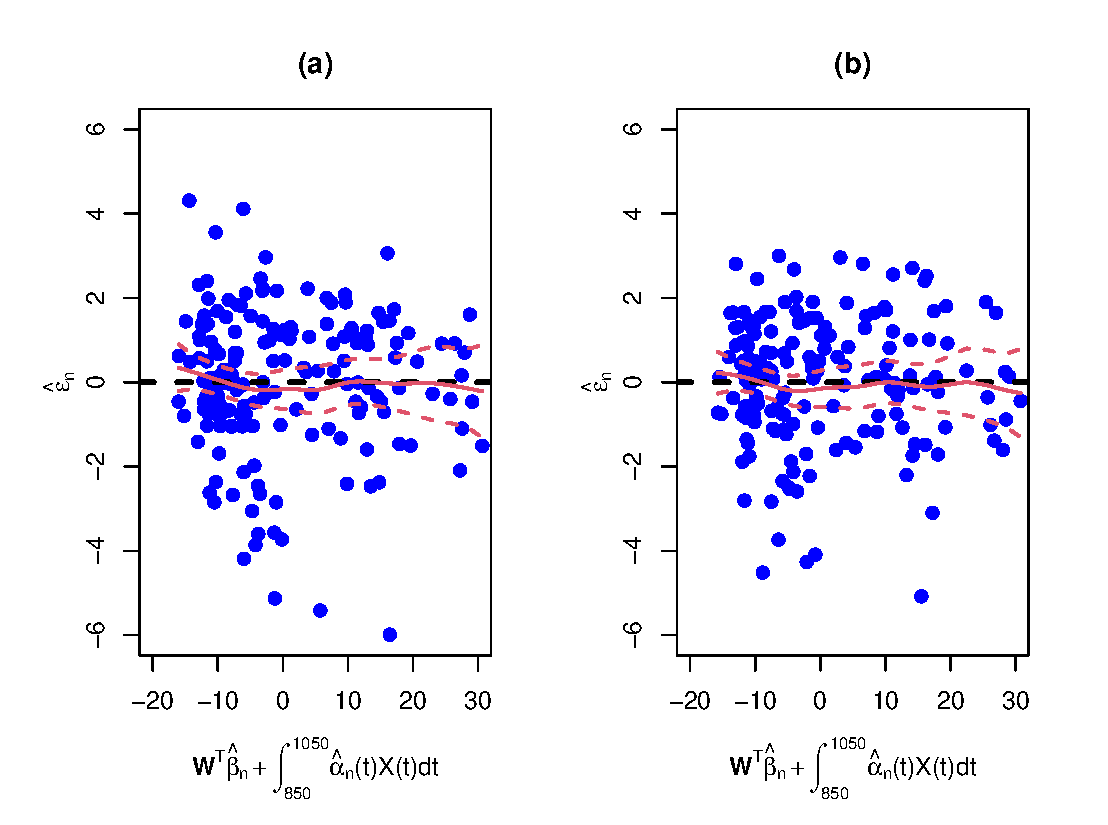
\includegraphics[width=1\textwidth,height=9cm]{rda221112.eps}
\caption{\scriptsize{{\color{blue}(a) Scatter plot of the calibrated model error estimator $\hat{\varepsilon}_n$ versus $\mathbf{W}^\top\hat{\beta}_n+\displaystyle\int_{850}^{1050}\hat{\alpha}_n(t)X(t)dt$ for Tecator data with $\Sigma_{u}=$diag$(3,0)$ by treating $\Sigma_{u}$ as known;  (b) Scatter plot of the calibrated model error estimator $\hat{\varepsilon}_n$ versus $\mathbf{W}^\top\hat{\beta}_n+\displaystyle\int_{850}^{1050}\hat{\alpha}_n(t)X(t)dt$ for Tecator data with $\Sigma_{u}=$diag$(3,0)$ by treating  $\Sigma_{u}$ as unknown.}
%;  (c) Scatter plot of the model error estimator $\hat{\varepsilon}_n^{NA}$ versus $\mathbf{W}^\top\hat{\beta}_n^{NA}+\displaystyle\int_0^1\hat{\alpha}_n^{NA}(t)X(t)dt$ for Tecator data with $\Sigma_{u}=$diag(3, 0)
}}
\end{figure}

		
\end{document}
